%; whizzy paragraph
%; whizzy-paragraph "^\\\\dancersection"
% -initex iniptex -latex platex -format platex -bibtex jbibtex -fmt fmt
% $B0J>e(B whizzytex $B$r;HMQ$9$k>l9g$N@_Dj!#(B

%     Tokyo Debian Meeting resources
%     Kansai Debian Meeting resources
%     Copyright (C) 2008 Junichi Uekawa
%     Copyright (C) 2008 Nobuhiro Iwamatsu

%     This program is free software; you can redistribute it and/or modify
%     it under the terms of the GNU General Public License as published by
%     the Free Software Foundation; either version 2 of the License, or
%     (at your option) any later version.

%     This program is distributed in the hope that it will be useful,
%     but WITHOUT ANY WARRANTY; without even the implied warranty of
%     MERCHANTABILITY or FITNESS FOR A PARTICULAR PURPOSE.  See the
%     GNU General Public License for more details.

%     You should have received a copy of the GNU General Public License
%     along with this program; if not, write to the Free Software
%     Foundation, Inc., 51 Franklin St, Fifth Floor, Boston, MA  02110-1301 USA

%   Pdf$B:n@.<j=g(B
% dvipdfmx debianmeetingresume2011-fuyu.dvi
%  preview (shell-command (concat "evince " (replace-regexp-in-string "tex$" "pdf"(buffer-file-name)) "&"))
% $B2hA|%U%!%$%k$r=hM}$9$k$?$a$K$O(Bebb$B$rMxMQ$7$F(Bboundingbox$B$r:n@.!#(B
%(shell-command "cd image2012-fuyu; ebb *.png")


% progress memo:
% 2016/6-2016/11$B$,%^!<%8BP>](B
% $B%$%Y%s%HEy$G$J$$>l9g$OM}M3$r=q$/$3$H!#(B
% $BI,MW$JJQ99E@$O(B FIXME $B$G5-O?$7$F$$$^$9!#(B

%%$B$3$3$+$i%X%C%@3+;O!#(B

\documentclass[mingoth,a4paper]{jsarticle}
\usepackage{monthlyreport}
\usepackage[dvips]{xy} % for advi workaround. Bug #452044
\usepackage{iwamatsu}
\usepackage{ulem}

% $B%3!<%I%O%$%i%$%H$N0Y$N@_Dj(B for 201606 tokyo
\makeatletter\chardef\pdf@shellescape=\@ne\makeatother
\usepackage{minted}

% $B%Z!<%8D4@0$N$?$aItJ,E*$K(B2$BCJAH$K(B
\usepackage{multicol}

\begin{document}

\begin{titlepage}
\thispagestyle{empty}

\hspace*{-2.5cm}
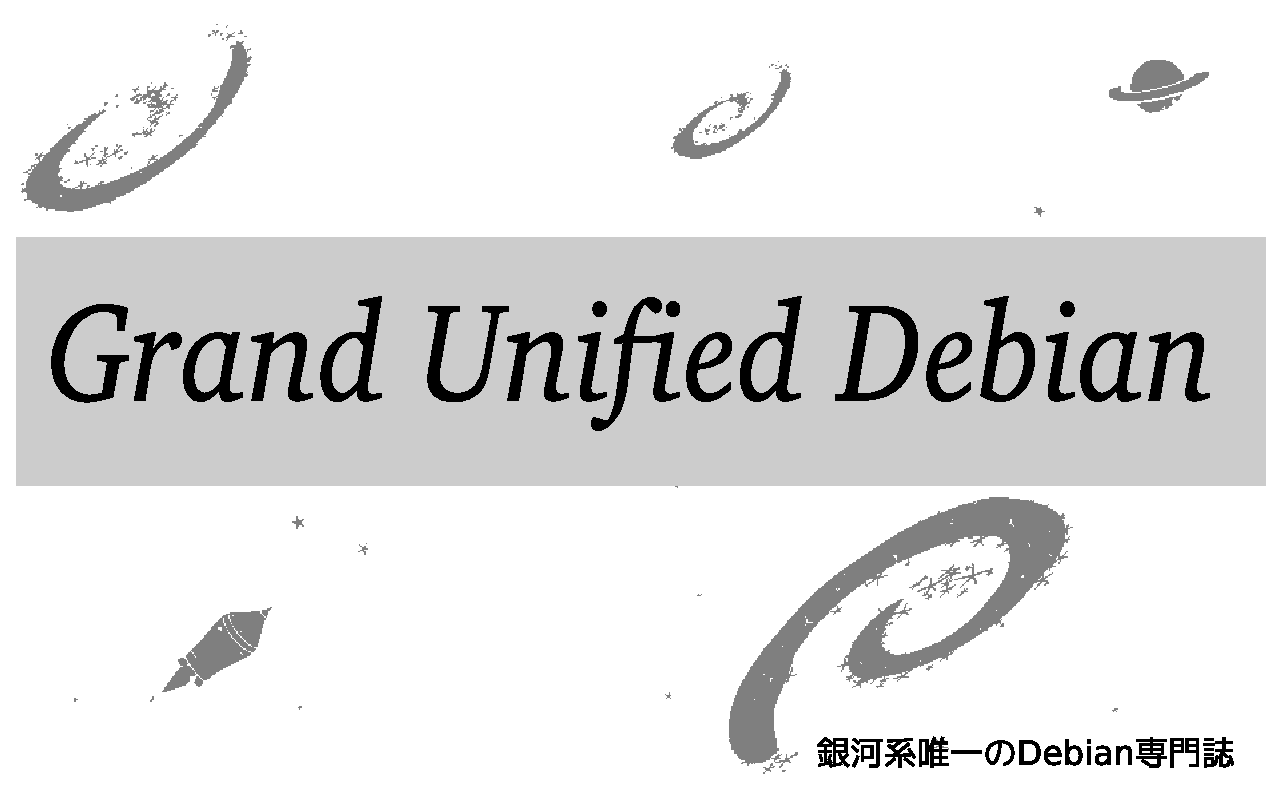
\includegraphics{image2012-natsu/gudeb.eps}\\
\\
\\
\rotatebox{10}{\fontsize{32}{32} {\gt $BEl5~%(%j%"(B/$B4X@>#D#e#b#i#a#nJY6/2q(B}}

%\vspace*{-1.5cm}
\hspace*{11cm}\includegraphics[height=6cm]{image200502/openlogo-nd.eps}\\
\vspace*{0.1cm}
\hfill $B$"$s$I$-$e$a$s$F$C$I(B $B$G$S$"$s(B 2016$BG/E_9f(B 2016$BG/(B12$B7n(B29$BF|(B $B=iHGH/9T(B
\end{titlepage}

\newpage
\thispagestyle{empty}\mbox{}
\newpage

% section $B$NBe$o$j$N4D6-(B -- $B2~D{$9$k!#(B
\renewcommand{\dancersection}[2]{%
\newpage
$B$"$s$I$-$e$a$s$F$C$I(B $B$G$S$"$s(B 2016$BG/E_9f(B
%
% top line
\vspace{0.1mm}\\
{\color{dancerlightblue}\rule{\hsize}{2mm}}

%
% middle text
%
\begin{minipage}[t]{0.6\hsize}
\color{dancerdarkblue}
\vspace{1cm}
\section{#1}
\hfill{}#2\\
\end{minipage}
\begin{minipage}[t]{0.4\hsize}
\vspace{-2cm}
\hfill{}\includegraphics[height=8cm]{image200502/openlogo-nd.eps}\\
\vspace{-5cm}
\end{minipage}
%
%
{\color{dancerdarkblue}\rule{0.74\hsize}{2mm}}
%
\vspace{2cm}
}

\setcounter{page}{1}
\begin{minipage}[]{0.2\hsize}
 \definecolor{titleback}{gray}{0.9}
 \colorbox{dancerlightblue}{\rotatebox{90}{\fontsize{80}{80}
{\gt \color{dancerdarkblue}$B%G%S%"%sJY6/2q(B} }}
\end{minipage}
\begin{minipage}[]{0.8\hsize}
\hrule
\vspace{1mm}
\hrule
\setcounter{tocdepth}{1}
{\small
 \tableofcontents}
\vspace{1mm}
\hrule
\vspace{3cm}

\end{minipage}

% FIXME: $BK\J8$rDI2C$9$k$3$H!#(B
%-------------------------------------------------------------------------------
\dancersection{Introduction}{DebianJP}
%-------------------------------------------------------------------------------

\subsection{$BEl5~%(%j%"(BDebian$BJY6/2q(B}

 Debian$BJY6/2q$X$h$&$3$=!#$3$l$+$i(BDebian$B$N@$3&$K$"$7$rF'$_F~$l$k$H(B
 $B$$$&J}$b!"$9$G$K$I$C$W$j$H$D$+$C$F$$$k$H$$$&J}$b!"7n$K0l2s(BDebian$B$K$D$$(B
 $B$F8l$j$^$;$s$+!)(B

 Debian$BJY6/2q$NL\E*$O2<5-$G$9!#(B

\begin{itemize}
 \item \underline{Debian Developer} ($B3+H/<T(B)$B$N0i@.!#(B
 \item $BF|K\8l$G$N(B ``\underline{$B3+H/$K4X$9$k>pJs(B}'' $B$r@0M}$7$F$^$H$a!"%"%C%W%G!<%H$9$k!#(B
 \item \underline{$B>l(B}$B$NDs6!!#(B
 \begin{itemize}
  \item $BIaCJ$P$i$P$i$J>l=j$K$$$k?M!9$,(B face-to-face $B$G=P2q$($k>l$rDs6!(B
    $B$9$k!#(B
  \item Debian $B$N$?$a$K$J$k$3$H$r8l$k>l$rDs6!$9$k!#(B
  \item Debian$B$K$D$$$F8l$k>l$rDs6!$9$k!#(B
 \end{itemize}
\end{itemize}

 Debian$B$NJY6/2q$H$$$&$3$H$G5f6KE*$K$O;22C<TA40w$,(BDebian Package$B$r$,$j$,$j(B
 $B$H:n$k%9!<%Q!<%O%C%+!<$K$J$C$?;Q$rLQA[$7$F$$$^$9!#>pJs$N6&M-!&3hMQ$rDL$7(B
 $B$F(B Debian$B$N:#8e$NG=F0E*$JE83+$X$NEZBf$H$7$F!"(B ``$B>l(B'' $B$H$7$F$N6u4V$rDs6!$9(B
 $B$k$N$,L\E*$G$9!#(B

\subsection{$B4X@>(B Debian $BJY6/2q(B}

 $B4X@>(B Debian $BJY6/2q$O(BDebian GNU/Linux $B$N$5$^$6(B
 $B$^$J%H%T%C%/(B($B?7$7$$%Q%C%1!<%8!"(BDebian $BFCM-$N5!G=$N;EAH!"(BDebian $B3&7($G5/(B
 $B$3$C$?=PMh;v!"$J$I$J$I!K$K$D$$$FOC$79g$&2q$G$9!#(B

 $BL\E*$H$7$F<!$N;0$D$r9M$($F$$$^$9!#(B
 \begin{itemize}
  \item ML$B$d7G<(HD$G$O$J$/!"D>@\4i$r9g$o$;$k;v$G$N>pJs8r49$NB%?J(B
  \item $BDj4|E*$K=8$^$l$k>l=j(B
  \item $B;qNA$N:n@.(B
 \end{itemize}

 $B$=$l$G$O!"3Z$7$$0l;~$r$*3Z$7$_2<$5$$!#(B

%201608 tokyo
%-------------------------------------------------------------------------------
\dancersection{Debian$B$G(Blxc$B$r%;%C%H%"%C%W$7$F$_$h$&(B}{$B?yK\(B $BE5=<(B}
%-------------------------------------------------------------------------------

\subsection{$B$O$8$a$K(B}

$B%3%s%T%e!<%?$N2>A[2=5;=Q$K%3%s%F%J7?2>A[2=$H$$$&;EAH$_$,$"$j$^$9!#K\H/I=$G$O!"%3%s%F%J7?2>A[2=5;=Q$N(B1$B$D$G$"$k(Blxc$B$K$D$$$F@bL@$7$^$9!#(B

\subsection{$B2>A[2=5;=Q$K$D$$$F(B}

\subsubsection{$B2>A[2=5;=Q$NJ,N`(B}

$B%3%s%T%e!<%?$K$*$1$k2>A[2=5;=Q$K$O$$$/$D$+$N<oN`$,$"$j$^$9!#(B

\begin{itemize}
  \item $B%3%s%F%J7?2>A[2=(B
  \begin{itemize}
  \item $B%2%9%H4D6-$O%[%9%H4D6-$N$"$k%G%#%l%/%H%j$KG[CV$7$?<B9T%U%!%$%k$*$h$S%i%$%V%i%j$N=89g$G$"$j!"<B9TCf$N%2%9%H4D6-$O%[%9%H4D6-$+$i8+$k$HC1$J$k%W%m%;%972$G$"$k!#<BAuNc$O(BOpenVZ$B!"(BLXC$B!#(B
  \end{itemize}
  \item $B=`2>A[2=7?(B
  \begin{itemize}
  \item $B%[%9%H4D6-$H$d$j$H$j$9$k(BAPI$B$rMxMQ$G$-$k$h$&$K=$@5$,F~$C$?(BOS$B$r%2%9%H4D6-$H$7$FF0:n$5$;$kJ}<0(B(=$B4{B8$N(BOS$B$=$N$^$^$G$OF0$+$J$$(B)$B!#<BAuNc$O(BXen$B!#(B
  \end{itemize}
  \item $B40A42>A[2=7?(B($B%(%_%e%l!<%7%g%s7?(B)
  \begin{itemize}
  \item $B4{B8$N(BOS$B$rL5=$@5$N$^$^%2%9%H4D6-$H$7$FF0:n$5$;$k!#%[%9%H4D6->e$GF0:n$9$k2>A[2=%"%W%j%1!<%7%g%s$,%2%9%H4D6-$r%(%_%e!<%7%g%s$9$k!#<BAuNc$O(BQEMU$B!"(BVirtualBox$B!#(B
  \end{itemize}
\item $B40A42>A[2=7?(B($B%O%$%Q!<%P%$%67?(B)
  \begin{itemize}
  \item $B4{B8$N(BOS$B$rL5=$@5$N$^$^%2%9%H4D6-$H$7$FF0:n$5$;$k!#(BCPU$B$N2>A[2=5!G=$r;H$&$3$H$G%[%9%H4D6-$K$*$1$k%*!<%P!<%X%C%I$r6KNO8:$i$7!"%(%_%e%l!<%7%g%s7?$h$j9b$$%Q%U%)!<%^%s%9$r=P$;$k!#<BAuNc$O(BKVM$B!#(B
  \end{itemize}
\end{itemize}

\subsubsection{$B2>A[2=5;=Q$N%a%j%C%H$H%G%a%j%C%H(B}

$B=`2>A[2=7?$*$h$S40A42>A[2=7?$K$*$1$k%2%9%H4D6-$OFCDj$N%O!<%I%&%'%"$r$b$DJ*M}%^%7%s$r%(%_%e%l!<%H$9$k$$$o$f$k!V2>A[%^%7%s!W$r<B9T$NC10L$H$7$^$9!#$=$N$?$a2>A[%^%7%s>e$G$b%+!<%M%k$r<B9T$5$;$kI,MW$,$"$j(BCPU$B!"%a%b%j!"%G%#%9%/$rB?$/;HMQ$7$^$9!#$=$NBe$o$j!"J*M}%^%7%s$XIaDL$K(BOS$B$r%$%s%9%H!<%k$7$F<B9T$7$F$$$?%W%m%0%i%`$r$=$N$^$^<B9T$G$-$k>l9g$,Hs>o$KB?$$$3$H$,M%0L$G$9!#(B

$B%3%s%F%J7?2>A[2=$K$*$1$k%2%9%H4D6-$O!"%[%9%H4D6-$N%+!<%M%k$GF0:n$9$k%W%m%;%972$G$"$k$?$a!"M>J,$J%+!<%M%k$d4IM}%G!<%b%s$rF0:n$5$;$kI,MW$,$J$/>J%j%=!<%9$GF0:n$G$-$kE@$,M%0L$G$9!#$=$NBe$o$j!"%[%9%H4D6-$N(BOS$B$d@_Dj$K$h$C$F%2%9%H4D6-$KF0:n@)Ls$,$D$/$3$H$,$"$j$^$9(B\footnote{raw$B%=%1%C%H$,MxMQ$G$-$J$$!"6&M-%a%b%j$,MxMQ$G$-$J$$!"(Bloopback$B$,MxMQ$G$-$J$$!"F10l%[%9%H4D6-$GF0:n$7$F$$$kB>$N%3%s%F%J$HDL?.$G$-$F$7$^$&!"$J$I$N@)Ls$,$"$k>l9g$,$"$j$^$9!#(B}$B!#(B

\subsubsection{$B%3%s%F%J7?2>A[2=5;=Q$N4pK\(Bchroot}

$B%3%s%F%J7?2>A[2=$N4pAC5;=Q$K(Bchroot$B$,$"$j$^$9(B\footnote{chroot$B%7%9%F%`%3!<%k$O(B1982$BG/$K%&%#%j%"%`!&%M%k%=%s!&%8%g%$(B($B%S%k!&%8%g%$$NL>$GCN$i$l$F$$$k(B)$B$,3+H/$7$?$3$H$r5/8;$H$5$l$F$$$^$9!#%S%k!&%8%g%$$O%W%m%0%i%`$r%/%j!<%s%S%k%I$G$-$k4D6-$,$[$7$+$C$?$?$aDL>oMxMQ$N4D6-$HJ,N%$9$k<jCJ$H$7$F3+H/$7$?$H8@$o$l$F$$$^$9!#(B}$B!#$"$k%G%#%l%/%H%jG[2<$K<B9T%U%!%$%k!"%i%$%V%i%j!"@_Dj%U%!%$%k$rE,@Z$KG[CV$7$?(Brootfs(=$B%3%s%F%J4D6-(B)$B$KBP$7$F(Bchroot(2)$B$^$?$O(Bchroot(3)$B$r<B9T$9$k$3$H$G!"%3%s%F%J4D6-Fb$N%i%$%V%i%j$r;H$C$F%3%^%s%I$r<B9T$G$-$^$9!#(B

\subsection{lxc$B2r@b(B}
\subsubsection{lxc$B$H$O(B}

lxc$B$H$O(B\footnote{LinuX Containers$B$r>JN,$7$F(Blxc$B$HFI$s$G$$$^$9!#(B}$B!"%3%s%F%J7?2>A[2=$H$7$FF0:n$9$kC10L$G$"$k%2%9%H4D6-(B(=rootfs)$B$NG[CV!"5/F0!"=*N;!"%3%s%=!<%kF~=PNO!"%M%C%H%o!<%/Ey$r4IM}$9$k;EAH$_$G$9!#(B
lxc$B$r;H$&$3$H$K$h$C$F!"%3%s%F%J4D6-$r5/F0$7!"(BIP$B%"%I%l%9$r3d$jEv$F!"$"$?$+$b$=$3$K(B1$BBf$N2>A[%^%7%s$,5/F0$7$?$+$N$h$&$K?6$kIq$&$3$H$,$G$-$^$9!#(B

\subsubsection{lxc$B$N%$%s%9%H!<%k(B}

$B:#2s$O(BDebian GNU/Linux 8 Jessie$B$N(Bamd64$B>e$G(Blxc$B$r%$%s%9%H!<%k$7$FF0:n$5$;$F$_$^$9!#(B
Debian Project$B$G$O0J2<$K%I%-%e%a%s%H$,$^$H$^$C$F$$$^$9!#(B

\begin{itemize}
\item https://wiki.debian.org/LXC
\item https://wiki.debian.org/LXC/SimpleBridge
\end{itemize}

$B$^$:!"(Blxc$B%Q%C%1!<%8$H2>A[%M%C%H%o!<%/$r9=C[$9$k%Q%C%1!<%8$r%$%s%9%H!<%k$7$^$9(B

\begin{commandline}
# apt-get install lxc bridge-utils libvirt-bin
\end{commandline}


lxc$B$r%$%s%9%H!<%k$9$k$H!"(Blxc-*$B%3%^%s%I$,;H$($k$h$&$K$J$j$^$9!#(B

\begin{commandline}
  $ ls /usr/bin/lxc*
  /usr/bin/lxc-attach       /usr/bin/lxc-start                   /usr/bin/lxc-test-list
  /usr/bin/lxc-autostart    /usr/bin/lxc-start-ephemeral         /usr/bin/lxc-test-locktests
  /usr/bin/lxc-cgroup       /usr/bin/lxc-stop                    /usr/bin/lxc-test-lxcpath
  /usr/bin/lxc-checkconfig  /usr/bin/lxc-test-apparmor           /usr/bin/lxc-test-may-control
  /usr/bin/lxc-clone        /usr/bin/lxc-test-attach             /usr/bin/lxc-test-reboot
  /usr/bin/lxc-config       /usr/bin/lxc-test-autostart          /usr/bin/lxc-test-saveconfig
  /usr/bin/lxc-console      /usr/bin/lxc-test-cgpath             /usr/bin/lxc-test-shutdowntest
  /usr/bin/lxc-create       /usr/bin/lxc-test-clonetest          /usr/bin/lxc-test-snapshot
  /usr/bin/lxc-destroy      /usr/bin/lxc-test-concurrent         /usr/bin/lxc-test-startone
  /usr/bin/lxc-device       /usr/bin/lxc-test-console            /usr/bin/lxc-test-symlink
  /usr/bin/lxc-execute      /usr/bin/lxc-test-containertests     /usr/bin/lxc-unfreeze
  /usr/bin/lxc-freeze       /usr/bin/lxc-test-createtest         /usr/bin/lxc-unshare
  /usr/bin/lxc-info         /usr/bin/lxc-test-destroytest        /usr/bin/lxc-usernsexec
  /usr/bin/lxc-ls           /usr/bin/lxc-test-device-add-remove  /usr/bin/lxc-wait
  /usr/bin/lxc-monitor      /usr/bin/lxc-test-get_item
  /usr/bin/lxc-snapshot     /usr/bin/lxc-test-getkeys
\end{commandline}

libvirt-bin$B$r%$%s%9%H!<%k$7$F(Blibvirtd$B$r5/F0$9$k$H!"%G%U%)%k%H$G(B192.168.122.0/24$B$N(BNAT$B%M%C%H%o!<%/$,9=@.$5$l$^$9!#:#2s$O:n@.$7$?%3%s%F%J4D6-$r$3$N(BNAT$B%M%C%H%o!<%/$K@\B3$7!"%[%9%H4D6-$H$D$J$,$k(B192.168.122.1(=virbr0)$B$r%G%U%)%k%H%2!<%H%&%'%$$H$7$FDL?.$G$-$k$h$&$K$7$^$9!#(B\footnote{$B2>A[%M%C%H%o!<%/$O%N!<%H%Q%=%3%s$d(BVPS$B$G9=C[$9$k>l9g$O(BNAT$B$NJ}$,$h$$$H;W$$$^$9$,!"<+Bp$d<RFb$N%M%C%H%o!<%/$G9=C[$9$k>l9g$O%V%j%C%8@\B3(B(=$B%[%9%H4D6-$H%3%s%F%J4D6-$,F10l%M%C%H%o!<%/$KB0$9$k7ABV(B)$B$rMxMQ$9$k$[$&$,$h$$>l9g$b$"$j$^$9!#(B}


$B<!$K!"(Blxc$B$GF0:n$9$k%3%s%F%J4D6-$K%j%=!<%9@)Ls$r9T$&;EAH$_$G$"$k(Bcgroups$B$r@_Dj$7$^$9!#(B

\begin{commandline}
  # vi /etc/fstab
  cgroup  /sys/fs/cgroup  cgroup  defaults  0   0

  # mount /sys/fs/cgroup
  # mount | grep cgroups
  cgroup on /sys/fs/cgroup/systemd type cgroup (rw,nosuid,nodev,noexec,relatime,xattr,
  release_agent=/lib/systemd/systemd-cgroups-agent,name=systemd)
\end{commandline}

$B$3$N>uBV$G!"(Blxc$B$r;H$($k4D6-$G$"$k$+3NG'$9$k%3%^%s%I(B"lxc-checkconfig"$B$r<B9T$7$F$_$^$9!#!V(Benabled$B!W$H=q$+$l$F$$$k$H$3$m$O!"<B:]$N%?!<%_%J%k>e$G$ONP?'$GI=<($5$l$^$9!#(Bdisable$B$N5!G=$O$"$j$^$;$s$N$G!"F0:n$G$-$k4D6-$G$"$k$3$H$,3NG'$G$-$^$7$?!#(B

\begin{commandline}
  # lxc-checkconfig
  Kernel configuration not found at /proc/config.gz; searching...
  Kernel configuration found at /boot/config-3.16.0-4-amd64
  --- Namespaces ---
  Namespaces: enabled
  Utsname namespace: enabled
  Ipc namespace: enabled
  Pid namespace: enabled
  User namespace: enabled
  Network namespace: enabled
  Multiple /dev/pts instances: enabled

  --- Control groups ---
  Cgroup: enabled
  Cgroup clone_children flag: enabled
  Cgroup device: enabled
  Cgroup sched: enabled
  Cgroup cpu account: enabled
  Cgroup memory controller: enabled
  Cgroup cpuset: enabled

  --- Misc ---
  Veth pair device: enabled
  Macvlan: enabled
  Vlan: enabled
  File capabilities: enabled

  Note : Before booting a new kernel, you can check its configuration
  usage : CONFIG=/path/to/config /usr/bin/lxc-checkconfig
\end{commandline}

\subsubsection{$B%3%s%F%J$N:n@.(B:lxc-create}

$B%2%9%H4D6-$H$J$k%3%s%F%J4D6-(B(=rootfs)$B$O(Blxc-create$B%3%^%s%I$G:n@.$9$k$3$H$,$G$-$^$9!#(B
$B:#2s$N(Blxc$B$N%3%s%F%J4D6-$O!"%[%9%H4D6-$HF1$8(BDebian GNU/Linux 8 Jessie amd64$B$r:n@.$7$^$9(B\footnote{$B%2%9%H4D6-$O!"%[%9%H4D6-$N(Blinux$B%+!<%M%k$GF0:n$9$k%P%$%J%j$G$"$l$P%[%9%H4D6-$H0[$J$k%G%#%9%H%j%S%e!<%7%g%s$G$bF0:n2DG=$G$9!#(B}$B!#:#2s$O!"(B''debstudy1''$B$H$$$&L>A0$G%3%s%F%J$r:n@.$7$^$9!#(B

\begin{commandline}
  # LANG=C SUITE=jessie MIRROR=http://ftp.jp.debian.org/debian lxc-create -n debstudy1 -t debian

  debootstrap is /usr/sbin/debootstrap
  Checking cache download in /var/cache/lxc/debian/rootfs-jessie-amd64 ...
  Copying rootfs to /var/lib/lxc/debstudy1/rootfs...Generating locales (this might take a while)...
  Generation complete.
  insserv: warning: current start runlevel(s) (empty) of script `checkroot.sh' overrides LSB defaults (S).
  insserv: warning: current stop runlevel(s) (S) of script `checkroot.sh' overrides LSB defaults (empty).
  insserv: warning: current start runlevel(s) (empty) of script `checkroot.sh' overrides LSB defaults (S).
  update-rc.d: error: umountfs Default-Start contains no runlevels, aborting.
  insserv: warning: current start runlevel(s) (empty) of script `hwclock.sh' overrides LSB defaults (S).
  insserv: warning: current stop runlevel(s) (0 6 S) of script `hwclock.sh' overrides LSB defaults (0 6).
  update-rc.d: error: cannot find a LSB script for hwclockfirst.sh
  Creating SSH2 RSA key; this may take some time ...
  2048 df:99:56:34:c7:6d:d1:0a:2d:e2:b4:6a:fd:a0:62:f5 /etc/ssh/ssh_host_rsa_key.pub (RSA)
  Creating SSH2 DSA key; this may take some time ...
  1024 9d:42:45:1d:fd:03:92:04:6c:e0:fb:e6:06:cc:07:06 /etc/ssh/ssh_host_dsa_key.pub (DSA)
  Creating SSH2 ECDSA key; this may take some time ...
  256 6a:4a:1a:6f:27:59:33:6c:58:5c:58:27:03:08:3b:ea /etc/ssh/ssh_host_ecdsa_key.pub (ECDSA)
  Creating SSH2 ED25519 key; this may take some time ...
  256 36:d6:9b:d3:9d:96:a4:af:af:8c:75:11:90:76:56:75 /etc/ssh/ssh_host_ed25519_key.pub (ED25519)
  Failed to read /proc/cmdline. Ignoring: No such file or directory
  invoke-rc.d: policy-rc.d denied execution of start.

  Current default time zone: 'Asia/Tokyo'
  Local time is now:      Sun Jul 10 13:26:07 JST 2016.
  Universal Time is now:  Sun Jul 10 04:26:07 UTC 2016.

  Root password is 'Won4EiUa', please change !
\end{commandline}

lxc-create$B$r<B9T$9$k$H!"(B''/var/lib/lxc/debstudy1''$B$H$$$&%G%#%l%/%H%j$,:n@.$5$l!"$=$NG[2<$K(Brootfs$B$H(Blxc$B$N%2%9%H4D6-MQ@_Dj%U%!%$%k$,@8@.$5$l$^$9!#(B
$B$J$*!"0lEY%3%s%F%J$r:n@.$9$k$H%@%&%s%m!<%I$7$?(Brootfs$B%U%!%$%k$O%-%c%C%7%e$5$l$^$9!#(B(2$B2sL\0J9_$N:n@.$G(BDebian$B%Q%C%1!<%8$N%@%&%s%m!<%I$,ITMW$K$J$jAa$/=hM}$,=*$o$j$^$9(B)

\begin{commandline}
  # ls -l /var/lib/lxc/debstudy1
  $B9g7W(B 8
  -rw-r--r--  1 root root  479  7$B7n(B 10 13:26 config
  -rw-r--r--  1 root root    0  7$B7n(B 10 13:26 fstab
  drwxr-xr-x 22 root root 4096  7$B7n(B 10 13:26 rootfs

  # ls /var/lib/lxc/debstudy1/rootfs
  bin  boot  dev  etc  home  lib  lib64  media  mnt  opt  proc  root  run  sbin  selinux  srv  sys  tmp  usr  var
\end{commandline}

lxc$B$,;2>H$9$k@_Dj%U%!%$%k$N=i4|>uBV$O0J2<$K$J$j$^$9!#(B

\begin{commandline}
  # cat /var/lib/lxc/debstudy1/config
  # Template used to create this container: /usr/share/lxc/templates/lxc-debian
  # Parameters passed to the template:
  # For additional config options, please look at lxc.container.conf(5)
  lxc.network.type = empty
  lxc.rootfs = /var/lib/lxc/debstudy1/rootfs

  # Common configuration
  lxc.include = /usr/share/lxc/config/debian.common.conf

  # Container specific configuration
  lxc.mount = /var/lib/lxc/debstudy1/fstab
  lxc.utsname = debstudy1
  lxc.arch = amd64
  lxc.autodev = 1
  lxc.kmsg = 0
\end{commandline}

$B$3$N(Bconfig$B%U%!%$%k$K%3%s%F%J4D6-$,MxMQ$9$k%M%C%H%o!<%/@_Dj$r9T$$$^$9!#(B

\begin{commandline}
  # vi /var/lib/lxc/debstudy1/config
  ($BKvHx$K0J2<$rDI2C(B)

  lxc.network.type = veth
  lxc.network.flags = up
  lxc.network.link = virbr0
  lxc.network.name = eth0
  lxc.network.ipv4 = 192.168.122.203/24
  lxc.network.ipv4.gateway = 192.168.122.1
\end{commandline}


\subsubsection{$B%3%s%F%J$N0lMw(B:lxc-ls}

lxc-ls$B%3%^%s%I$G:n@.$7$?%3%s%F%J$N0lMw$rI=<($G$-$^$9!#(B

\begin{commandline}
  # lxc-ls
  debstudy1
\end{commandline}


\subsubsection{$B%3%s%F%J$N:o=|(B:lxc-destroy}

lxc-destroy$B%3%^%s%I$G%3%s%F%J$r:o=|$G$-$^$9!#(B

\begin{commandline}
  # lxc-destroy -n <lxc-name>
\end{commandline}


\subsubsection{$B%3%s%F%J$N5/F0(B:lxc-start}

lxc-start$B%3%^%s%I$G%3%s%F%J$r5/F0$7$^$9!#%3%s%F%J$r5/F0$9$k$H!"%3%s%F%J4D6-Fb$K$"$k(Binit$B%W%m%0%i%`$,<B9T$5$l>oCs$7$^$9!#(B

-d$B%*%W%7%g%s$O%3%s%F%J4D6-$r%P%C%/%0%i%&%s%I$G5/F0$9$k%*%W%7%g%s$G$9!#(B-d$B%*%W%7%g%s$rIU$1$J$$>l9g!"(Blxc-start$B$r<B9T$7$?%?!<%_%J%k$O%3%s%F%J4D6-$N%3%s%=!<%k$K@\B3$5$l$^$9!#(B

\begin{commandline}
  # lxc-start -n debstudy1
  $B!!$^$?$O(B
  # lxc-start -n debstudy1 -d
\end{commandline}


\subsubsection{$B%3%s%F%J$N=*N;(B:lxc-stop}

lxc-stop$B%3%^%s%I$G%3%s%F%J$r=*N;$7$^$9!#%3%s%F%J$r=*N;$9$k$H!"(Binit$B%W%m%0%i%`$,5/F0Cf$N%G!<%b%s$r=*N;$5$;!"(Binit$B%W%m%0%i%`<+?H$b=*N;$7$^$9!#(B

\begin{commandline}
  # lxc-stop -n debstudy1
\end{commandline}

\subsubsection{$B%3%s%F%J$N%3%s%=!<%k$X@\B3$9$k(B:lxc-console}

lxc-console$B%3%^%s%I$G%3%s%F%J4D6-$N%3%s%=!<%k$X@\B3$7$^$9!#(B

``Ctrl+a q''$B$N=g$K%-!<F~NO$9$k$H!"%3%s%=!<%k$+$iH4$1$k$3$H$,$G$-$^$9!#(B

\begin{commandline}
  # lxc-console -n debstudy1

  Connected to tty 1
  Type <Ctrl+a q> to exit the console, <Ctrl+a Ctrl+a> to enter Ctrl+a itself

  Debian GNU/Linux 8 debstudy1 tty1

  debstudy1 login:
\end{commandline}


\subsection{lxc$B$r<BMQ$9$k(B}
\subsubsection{lxc$B$N%2%9%H4D6-$r$rMxMQ2DG=$J>uBV$^$G%;%C%H%"%C%W$9$kN.$l(B}

lxc$B$N%2%9%H4D6-$X$N%m%0%$%s$O(Bssh$B$G%m%0%$%s$7$?$$$H;W$&$3$H$,B?$$$H9M$($^$9!#(B
$B$=$N$?$a!"(Blxc$B$N%2%9%H4D6-$r:n@.$7$FF0:n$5$;$k$^$G$N%;%C%H%"%C%W$NN.$l$N0lNc$r$^$H$a$F$_$^$9!#(B

$B$J$*!"(Bdebian$B$N>l9g$O(Blxc-create$B$7$?$H$-$N(Brootfs$BFb$K(Bopenssh-server$B%Q%C%1!<%8$b%$%s%9%H!<%k$5$l$^$9!#(B

\begin{itemize}
\item lxc-create$B%3%^%s%I$G%2%9%H4D6-$r:n@.$9$k(B
\item config$B%U%!%$%k$r=$@5$7!"(BIP$B%"%I%l%9IUM?5Z$S%M%C%H%o!<%/@_Dj$r9T$&(B
\item chroot$B%3%^%s%I$G(Brootfs$B$XD>@\F~$k(B($B$^$?$O!"(Blxc-start$B$G%3%s%F%J4D6-$r5/F0$7$F%3%s%=!<%k$X@\B3$9$k(B)
  \begin{itemize}
  \item passwd$B%3%^%s%I$G(Broot$B%Q%9%o!<%I$r=q$-49$($k(B
  \item adduser$B%3%^%s%I$G%f!<%6$r:n@.$9$k(B
  \item apt-get install sudo vim-tiny
  \item visudo
  \item dpkg-reconfigure locales  ($B=i4|CM$O(Blxc-create$B$7$?$H$-$K(BLANG$BCM$H$J$j$^$9(B)
  \end{itemize}
\item lxc-start -n \{lxc-name\} -d $B$r<B9T$7!"%P%C%/%0%i%&%s%I$G%2%9%H4D6-$r5/F0(B
\item $B%[%9%H4D6-$+$i(Bssh$B%3%^%s%I$G%2%9%H4D6-$N(BIP$B%"%I%l%9$H%f!<%6$r;XDj$7$F%m%0%$%s$9$k(B
\end{itemize}

ssh$B%m%0%$%s$,$G$-!"(Bsudo$B$,MxMQ$G$-$k$h$&$K$J$l$P8e$O$*9%$_$G@_Dj$,$G$-$k$H;W$$$^$9!#(B

\newpage

\subsubsection{$B2?$K(Blxc$B$r;H$&$+(B}

lxc$B$r$I$N$h$&$J>lLL$GMxMQ$9$k$+$O$=$N?M<!Bh$G$9!#<+J,$O0J2<$NMQES$GMxMQ$7$F$$$^$9!#(B

\begin{itemize}
\item $B0l;~E*$J8!>Z$G!"%[%9%H4D6-$K$$$m$$$m%$%s%9%H!<%k$7$?$/$J$$>l9g(B($BNc!'%G!<%b%s$N:F5/F0$,I,MW$K$J$k(B)
\item python2$B7O$H(Bpython3$B7O$,:.:_$7$?J#?t$N(Bweb$B%"%W%j%1!<%7%g%s$r(B1$B$D$N%[%9%H$GF0$+$7$?$$>l9g(B(debian$B$N>l9g!"(Blibapache2-mod-wsgi$B$H(Blibapache2-mod-wsgi-py3$B$O6&B8$G$-$J$$(B)
\item $B%[%9%H4D6-$O(Bsystemd$B$N$^$^$G!"%2%9%H4D6-$O(Bsysvinit$B$GF0:n$5$;$?$$>l9g(B(systemd$B$KBP1~$7$J$$%W%m%0%i%`$rMxMQ$9$k6lFy$N:v(B)
\item $B3+H/$7$?%"%W%j%1!<%7%g%s$r%/%j!<%s$J4D6-$G%S%k%I$d%$%s%9%H!<%k$G$-$k$+%F%9%H$r9T$&>l9g(B\footnote{$B$-$A$s$H(Bdebian$B%Q%C%1!<%8$K$7$F%$%s%9%H!<%k$9$k$h$&$K$9$l$P!"$3$NMQES$GMxMQ$9$k$3$H$O$J$$$O$:$G$9!#(B}\footnote{debian$B$K$"$k(Bpbuilder$B$d(Bcowbuilder$B$O%/%j!<%s$J(Brootfs$B$X(Bchroot$B$7$F(Bdebian$B%Q%C%1!<%8$N%S%k%I$,$G$-$k$+$r%F%9%H$9$kJXMx%3%^%s%I$G$9!#(B}
\item amd64$B>e$G(Bi386$B4D6-$,$[$7$$!"$^$?$O0[$J$k(BCPU$B%"!<%-%F%/%A%c$N%3%s%F%J4D6-$,F0:n$9$k%/%m%94D6-$,$[$7$$>l9g(B\footnote{cross debootstrap$B$H$$$$!"(BQEMU$B$HAH$_9g$o$;$^$9!#(B}
\end{itemize}


\subsection{$B$*$o$j$K(B}

Debian GNU/Linux$B>e$G(Blxc$B$r;n$7$F$_$^$7$?!#(Blxc$B$O!"J#?t%[%9%H$N(Blxc$B4D6-$r@)8f$9$k(BLXD$B$d(Bdocker$B$N4pAC5;=Q$G$"$k$?$a!"3'$5$^;n$7$F$_$F$/$@$5$$!#(B


\subsection{$B;29MJ88%(B}

\begin{itemize}
  \item $B!V(BLXC$B!W(B \url{https://linuxcontainers.org/}
  \item $B!V(BLXC - Debian Wiki$B!W(B \url{https://wiki.debian.org/LXC}
  \item $B?yK\(B $BE5=<(B (2013) $B!V(Bdebootstrap$B$rM-8z3hMQ$7$F$_$h$&!W(B \url{http://tokyodebian.alioth.debian.org/pdf/debianmeetingresume201304.pdf}
\end{itemize}
%-------------------------------------------------------------------------------
\dancersection{preseed$B$G(BDebian$B$r<+F0%$%s%9%H!<%k$r$7$F$_$h$&(B}{$B?yK\E5=<(B}
%-------------------------------------------------------------------------------

\subsection{$B$O$8$a$K(B}

$B2>A[2=5;=Q$,?J$_!"(BOS$B$r%$%s%9%H!<%k$9$k5!2q$,8:$C$??M!"A}$($??M$H$=$l$>$l3'MM$N;v>p$,$"$k$H;W$$$^$9!#(B
$B:#2s$O(BDebian$B$r%$%s%9%H!<%k$9$k5!2q$,B?$$J}$K8~$1$F%$%s%9%H!<%k:n6H$r<+F0$G9T$&(Bpreseed$B5!G=$r$4>R2p$7$^$9!#(B

\subsection{debian$B$r%$%s%9%H!<%k$9$kJ}K!(B}

Debian$B$r(BPC$B$d%5!<%P$X%$%s%9%H!<%k$9$k>l9g$O!"(BDebian Installer$B$r;H$&$3$H$,B?$$$G$9!#(B\footnote{$B%\!<%I%G%P%$%9$N$h$&$K(BDebian Installer$B$r;H$o$J$$$G%$%s%9%H!<%k$7$F$$$kLT<T$b$$$^$9!#(B}

Debian Installer$B$O0J2<$N7A<0$GDs6!$5$l$F$*$j!">u67$K$h$C$F;H$$J,$1$k$3$H$rA[Dj$7$F$$$^$9!#(B

\begin{itemize}
\item $B$9$Y$F$N(BDebian$B%Q%C%1!<%8$r<}O?$7$?%$%a!<%8!#(BCD, DVD, Blu-ray$B$N(BISO$B7A<0$GDs6!!#(B
\item $B%M%C%H%o!<%/%$%s%9%H!<%kMQ$N%V!<%H%$%a!<%8!#DL>N(Bnetinst$B%$%a!<%8!#(BCD$B$N(BISO$B7A<0!"(BUSB$B%a%b%j7A<0$GDs6!!#(B
\item vmlinuz$B!"(Binitrd.gz$B%U%!%$%k$rC1BN$GDs6!!#2>A[2=4D6-$d%\!<%I%G%P%$%98~$1!#(B
\end{itemize}

$BF|>o4D6-$GMxMQ$9$k>l9g$O:G?7%P!<%8%g%s$rMxMQ$9$k$H;W$$$^$9$N$G!"%M%C%H%o!<%/%$%s%9%H!<%kMQ%$%a!<%8$r;H$&$3$H$r$*4+$a$7$^$9!J%M%C%H%o!<%/$+$i:G?7$N%Q%C%1!<%8$r%@%&%s%m!<%I$7$F%$%s%9%H!<%k$9$k$?$a$G$9!K!#(B


\subsection{preseed}
\subsubsection{preseed$B$H$O(B}

preseed$B$H$O!"(BDebian Installer$B$N!V%$%s%9%H!<%k$N<B9TCf$K<jF0$G2sEz$rF~NO$;$:$K!"%$%s%9%H!<%k%W%m%;%9Cf$N<ALd$NEz$r@_Dj$9$kJ}K!$rDs6!!W$9$k5!G=$r$$$$$^$9!#(B\footnote{https://www.debian.org/releases/jessie/amd64/apb.html.ja}

preseed$B5!G=$G$O!"%$%s%9%H!<%k=hM}$N%Q%i%a!<%?$rDj5A$7$?F~NO%U%!%$%k$,I,MW$K$J$j$^$9!#$=$N%U%!%$%k$N%G%U%)%k%H$N%U%!%$%kL>$O(Bpreseed.cfg$B$H$J$C$F$$$^$9!#(B

\subsubsection{preseed$B$N<oN`(B}

preseed$B5!G=$O(B3$B<oN`$KJ,$+$l$F$*$j!"(Bpreseed.cfg$B$rFI$_9~$`J}K!$d%?%$%_%s%0$,0[$J$j$^$9!#(B

\begin{itemize}
\item initrd preseed
  \begin{itemize}
  \item Debian Installer$B$N(Binitrd.gz$B$NCf$K(B/preseed.cfg$B$rDI2C$GG[CV$9$k(B
  \item $B%$%s%9%H!<%i5/F0D>8e$NA*Br;h$+$i(B/preseed.cfg$B$NDj5A$K=>$$<+F0%$%s%9%H!<%k$9$k(B
  \end{itemize}
\item file preseed
  \begin{itemize}
  \item Debian Installer$B$N(BISO$B%U%!%$%k$NCf$K(B/preseed.cfg$B$rDI2C$GG[CV$9$k!J!aMW%j%^%9%?%j%s%0!K(B
  \item Debian Installer$B$N(BUSB$B%a%b%j$NCf$K(B/preseed.cfg$B$rDI2C$GG[CV$9$k(B
  \item Debian Installer$B$N(Bkernel$B%V!<%H%Q%i%a!<%?$K(Bpreseed/file$B!"(Bpreseed/file/checksum$B$r;XDj$9$kI,MW$,$"$k(B
  \end{itemize}
\item network preseed
  \begin{itemize}
  \item IP$B%"%I%l%9$N<hF@$^$?$O@_Dj8e$K(Bpreseed.cfg$B$r(Bwget$B$G%@%&%s%m!<%I$7$FFI$_9~$`(B
  \item Debian Installer$B$N(Bkernel$B%V!<%H%Q%i%a!<%?$K(Bpreseed/url$B!"(Bpreseed/url/checksum$B$r;XDj$9$kI,MW$,$"$k(B
  \item Debian Installer$B$G$O(BIP$B%"%I%l%9$r@_Dj$9$kA0$K$bA*Br;h$,=P$F$/$k$?$a!"40A4$J<+F0%$%s%9%H!<%k$r$9$k$K$ODI2C$N(Bkernel$B%V!<%H%Q%i%a!<%?$,I,MW(B
  \end{itemize}
\end{itemize}


\subsubsection{preseed$B%U%!%$%k$N;EMM(B}

preseed$B%U%!%$%k$G;XDj$G$-$k%Q%i%a!<%?$N2r@b$O0J2<$K>\$7$/=q$+$l$F$$$^$9!#(B

\begin{itemize}
\item $B!V(BB.4. $B;vA0@_Dj%U%!%$%k$NFbMF(B (jessie $BMQ(B)$B!W(B
  \begin{itemize}
  \item \url{https://www.debian.org/releases/stable/amd64/apbs04.html.ja}
  \end{itemize}
  \item $B!V(BB.2.4. preseed $B$GMxMQ$G$-$k%(%$%j%"%9!W(B
  \begin{itemize}
  \item \url{https://www.debian.org/releases/stable/amd64/apbs02.html.ja#preseed-aliases}
  \end{itemize}
\end{itemize}

Debian-8(jessie)$BMQ$N%5%s%W%k(Bpreseed$B%U%!%$%k$O0J2<$GDs6!$7$F$$$^$9!#(B

\begin{itemize}
\item \url{https://www.debian.org/releases/jessie/example-preseed.txt}
\end{itemize}


\subsubsection{$B%$%s%9%H!<%kCf$N%+%9%?%`%3%^%s%I<B9T(B}

preseed$B$G<+F0%$%s%9%H!<%k$r$7$F$$$k$H$-$KG$0U$J=hM}!J!a%+%9%?%`%3%^%s%I!K$r<B9T$9$k5!G=$,$"$j$^$9!#%+%9%?%`%3%^%s%I$N<B9T%?%$%_%s%0$O0J2<$N(B3$B%Q%?!<%s$r;XDj$G$-$^$9!#(B

\subsubsubsection{preseed/early\_command}

$BA4BN$N%$%s%9%H!<%k=hM}$,;O$^$kA0$K%3%^%s%I$r<B9T$7$?$$>l9g$O!"(B"preseed/early\_command"$B$G;XDj$G$-$^$9!#(B

\begin{commandline}
d-i preseed/early_command string anna-install some-udeb
\end{commandline}

\subsubsubsection{$B=hM}L>(B/early\_command}

$B$"$k=hM}$N<B9TA0$K%3%^%s%I$r<B9T$7$?$$>l9g$O!"(B"$B=hM}L>(B/early\_command"$B$G;XDj$G$-$^$9!#(B

\begin{commandline}
d-i partman/early_command string debconf-set partman-auto/disk ``$(list-devices disk | head -n1)''
\end{commandline}

\subsubsubsection{preseed/late\_command}

$B%$%s%9%H!<%k$,40N;$7$F:F5/F0$9$kA0$K%3%^%s%I$r<B9T$7$?$$>l9g$O!"(B"preseed/late\_command"$B$G;XDj$G$-$^$9!#$J$*!"$3$N>u67$G$O%$%s%9%H!<%k@h%G%#%9%/$N(B/$B%Q!<%F%#%7%g%s$,(B/target$B$X%^%&%s%H$7$?>uBV$K$J$C$F$$$^$9!#(B

\begin{commandline}
d-i preseed/late_command string apt-install zsh; in-target chsh -s /bin/zsh
\end{commandline}


\subsection{preseed$B$r;H$C$F(Bdebian$B$r%$%s%9%H!<%k$9$k(B}

\subsubsection{$B%$%s%9%H!<%k$9$k4D6-(B}

$B%$%s%9%H!<%k$9$k%[%9%H9=@.$H%M%C%H%o!<%/9=@.$O0J2<$N4D6-$H$7$^$9!#(B

\begin{itemize}
\item Debian GNU/Linux 8$B$N(BKVM$B%[%9%H4D6-$r=`Hw(B
\item $B%$%s%9%H!<%k$9$k%[%9%H$O!"(BKVM$B$N2>A[%^%7%s$H$9$k(B
  \begin{itemize}
  \item $B%M%C%H%o!<%/%+!<%I$O(B1$B$D(B
  \item $B%G%#%9%/$N@\B3%P%9$O(Bsata\footnote{KVM$B$r;H$&>l9g$O%G%#%9%/$N@\B3%P%9$r(Bvirtio$B$K$9$kJ}$,@-G=$O$h$$$G$9!#(Bvirtio$B$r;H$&>l9g$O(Bpreseed$B$NDj5A$K$"$k(B/dev/sda$B$NItJ,$r(B/dev/vda$B$KJQ99$9$k$3$H$rK:$l$J$$$G$/$@$5$$!#(B}
  \item KVM$B%[%9%H$+$i(BKVM$B%2%9%H$X$N@\B3$O%7%j%"%k%3%s%=!<%k@\B3$H$9$k(B
  \end{itemize}
\end{itemize}

\subsubsection{$B:#2s:n@.$7$?(Bpreseed.cfg$B%U%!%$%k(B}

$B0J2<$N(Bpreseed.cfg$B%U%!%$%k$N@_Dj$G<+F0%$%s%9%H!<%k$7$^$9!#(B

\begin{commandline}
  d-i debian-installer/language string C
  d-i debian-installer/country string JP
  d-i debian-installer/locale string ja_JP.UTF-8
  d-i keyboard-configuration/xkb-keymap select jp
  d-i netcfg/enable boolean true
  d-i netcfg/choose_interface select auto
  d-i netcfg/get_hostname string deb-preseed
  d-i netcfg/get_domain string localdomain
  d-i netcfg/hostname string dev-preseed
  d-i netcfg/wireless_wep string
  d-i hw-detect/load_firmware boolean false
  d-i mirror/country string manual
  d-i mirror/http/hostname string ftp.jp.debian.org
  d-i mirror/http/directory string /debian
  d-i mirror/http/proxy string
  d-i mirror/suite string jessie
  d-i passwd/root-login boolean true
  d-i passwd/make-user boolean true
  d-i passwd/root-password password rootpass
  d-i passwd/root-password-again password rootpass
  d-i passwd/user-fullname string Test User
  d-i passwd/username string testuser
  d-i passwd/user-password password testpass
  d-i passwd/user-password-again password testpass
  d-i passwd/user-default-groups string audio cdrom video sudo
  d-i clock-setup/utc boolean true
  d-i time/zone string Asia/Tokyo
  d-i clock-setup/ntp boolean true
  d-i clock-setup/ntp-server string ntp.nict.jp
  d-i partman-auto/init_automatically_partition select biggest_free
  d-i partman-auto/disk string /dev/sda
  d-i partman-auto/method string regular
  d-i partman-lvm/device_remove_lvm boolean true
  d-i partman-md/device_remove_md boolean true
  d-i partman-lvm/confirm boolean true
  d-i partman-lvm/confirm_nooverwrite boolean true
  d-i partman-auto/choose_recipe select atomic
  d-i partman-partitioning/confirm_write_new_label boolean true
  d-i partman/choose_partition select finish
  d-i partman/confirm boolean true
  d-i partman/confirm_nooverwrite boolean true
  d-i partman-md/confirm boolean true
  d-i partman-partitioning/confirm_write_new_label boolean true
  d-i partman/choose_partition select finish
  d-i partman/confirm boolean true
  d-i partman/confirm_nooverwrite boolean true
  d-i partman/mount_style select uuid
  d-i base-installer/install-recommends boolean false
  d-i base-installer/kernel/image string linux-image-amd64
  d-i apt-setup/non-free boolean false
  d-i apt-setup/contrib boolean true
  d-i apt-setup/use_mirror boolean true
  tasksel tasksel/first multiselect ssh-server
  d-i pkgsel/include string ntp ntpdate sudo curl
  d-i pkgsel/upgrade select none
  popularity-contest popularity-contest/participate boolean false
  d-i grub-installer/skip boolean false
  d-i grub-installer/only_debian boolean true
  d-i grub-installer/with_other_os boolean true
  d-i grub-installer/bootdev  string /dev/sda
  d-i debian-installer/add-kernel-opts string console=ttyS0,115200n8
  d-i finish-install/reboot_in_progress note
  d-i cdrom-detect/eject boolean true
  d-i preseed/late_command string \
  in-target /usr/bin/curl http://192.168.22.102/preseed/done.cgi
\end{commandline}


\subsubsection{netinst$B%$%a!<%8$r;H$C$?<+F0%$%s%9%H!<%k(B}

netinst$BMQ(BISO$B%U%!%$%k$+$i%V!<%H$7$F%$%s%9%H!<%k$9$k>l9g$O!"(BDebian Installer$B$N(Bkernel$B%V!<%H%Q%i%a!<%?$K0J2<$N$h$&$J%3%^%s%I$rDI2C$G;XDj$7$^$9!#(B

\begin{commandline}
auto=true priority=critical url=http://192.168.22.41/preseed.cfg preseed/url/checksum=8e85ff2ddb966321b91f13f9aba9dc9f
\end{commandline}

preseed/url/checksum$B$O(Bmd5sum$B$J$N$G$9$,!";XDj$,I,?\$H$J$C$F$$$k$?$aCm0U$7$J$,$iF~NO$7$^$9!#$b$7(Bchecksum$B$,9g$o$J$$>l9g$O(Bpreseed.cfg$B%U%!%$%k$OL58z$HH=Dj$5$l$k;EMM$K$J$C$F$$$^$9(B\footnote{$B$=$N>l9g$O!"%$%s%9%H!<%k$,%9%H%C%W$7$?$j!"<jF0$G%$%s%9%H!<%k>l9g$HF1$8$/<ALd$KEz$($k2hLL$GF~NOBT$A>uBV$K$J$j$^$9!#(B}$B!#(B


\subsubsection{virt-install$B$r;H$C$?<+F0%$%s%9%H!<%k(B}

KVM$B$N2>A[%^%7%s$r%$%s%9%H!<%k$9$k%3%^%s%I$K(B"virt-install"$B$,$"$j$^$9!#$3$N(Bvirt-install$B$r;H$C$F(BKVM$B%2%9%H%^%7%s$N%$%s%9%H!<%k$K(Bpreseed$B$r;H$&>l9g$O!"(B"--initrd-inject"$B%*%W%7%g%s$r;XDj$7$^$9!#(B

"-initrd-inject"$B%*%W%7%g%s$O(Binitrd.gz$B$NCf$K;XDj$7$?%U%!%$%k$rG&$S9~$^$;$k$3$H$,$G$-$^$9!#$J$*!"$3$N%$%s%9%H!<%kJ}K!$N>l9g$O(BDebian Installer$B$N%V!<%H;~$K(B/preseed.cfg$B%U%!%$%k$,B8:_$9$k$3$H$+$i(Binitrd preseed$B$NF0:n$G%$%s%9%H!<%k=hM}$,?J$_$^$9!#(B

\begin{commandline}
$ sudo virt-install \
  --name deb-preseed-1 \
  --disk path=/var/lib/libvirt/images/deb-preseed-1.img,format=qcow2,bus=sata \
  --vcpus 1 --ram 1024 \
  --network bridge=br0,model=e1000 \
  --graphics none \
  --os-type linux --os-variant generic \
  --console pty,target_type=serial \
  --location 'http://ftp.jp.debian.org/debian/dists/jessie/main/installer-amd64/' \
  --initrd-inject=/var/lib/libvirt/images/preseed.cfg \
  --extra-args 'console=ttyS0,115200n8 serial'
\end{commandline}


\subsection{$B$^$H$a(B}

Debian$B$K$"$k(Bpreseed$B5!G=$r;H$C$F<+F0%$%s%9%H!<%k$r;n$7$F$_$^$7$?!#(BKVM$B$J$I$N2>A[4D6-$r07$C$F$$$FF|>oE*$K(BDebian$B$r%$%s%9%H!<%k$7$F$$$k>l9g$O8zN(E*$K:n6H$,$G$-$k$H;W$$$^$9$N$G3hMQ$7$F$_$F$/$@$5$$!#(B

\subsection{$B;29MJ88%(B}

\begin{itemize}
\item $B!V(BDebianInstallerPreseed$B!W(B \url{https://wiki.debian.org/DebianInstaller/Preseed}
\item $B!VIUO?(BB preseed $B$rMxMQ$7$?%$%s%9%H!<%k$N<+F02=!W(B \url{https://www.debian.org/releases/jessie/amd64/apb.html.ja}
\end{itemize}

\dancersection{Let's Encrypt $B$N%9%9%a(B}{$B$+$o$@(B $B$F$D$?$m$&(B}

\subsection{$B$O$8$a$K(B}

$BL5NA$G(BSSL/TLS$B>ZL@=q$r<hF@$G$-$k%5!<%S%9$H$7$F(BStart SSL$B$d(BWo Sign$B!"(BCAcert$B$J$I$$$/(B
$B$D$+$"$j$^$9$,!":#2s$O(BDebian$B%Q%C%1!<%8$r;HMQ$7$F4JC1$KF3F~$G$-$k(BLet's Encrypt$B$r(B
$B>R2p$7$^$9!#(B


\subsection{Let's Encrypt$B$K$D$$$F(B}

Let's Encrypt\footnote{\url{https://letsencrypt.org/}}$B$O(B2016$BG/(B4$B7n(B12$BF|$K%5!<%S%9(B
$B$r3+;O$7$?G'>Z6I(B(CA)$B$G$9!#F|K\8l$N>pJs$O!V(BLet's Encrypt $BAm9g%]!<%?%k(B
\footnote{\url{https://letsencrypt.jp/}}$B!W$K$^$H$^$C$F$$$^$9$N$G;2>H$7$F$/$@$5$$!#(B

$B$=$NFCD'$H$7$F(B
\begin{itemize}
\item $B%U%j!<$G<+F02=$5$l$?%*!<%W%s$JG'>Z6I(B
\item $BHs1DMxCDBN(BISRG(Internet Security Research Group)$B$,1?1D(B
\item ACME(Automated Certificate Management Environment)$B%W%m%H%3%k(B
\end{itemize}
$B$,$"$2$i$l$^$9!#(B

\subsubsection{$B>ZL@=q(B}

$BH/9T$5$l$k>ZL@=q$O!"%I%a%$%sG'>Z(B(DV:Domain Validation)$B>ZL@=q$G$9!#(B
$B4k6HG'>Z(B(OV:Organization Validation)$B>ZL@=q$d(BEV(Extended Validation)$B>ZL@=q$OH/9T(B
$B$5$l$^$;$s!#%o%$%k%I%+!<%I>ZL@=q$K$OBP1~$7$F$$$^$;$s$,!"J#?t$N%5%V%I%a%$%sL>$N>Z(B
$BL@=q$,<hF@$G$-$^$9$N$GLdBj$K$O$J$i$J$$$G$7$g$&!#(B

$B%k!<%H>ZL@=q$O!"(BIdenTrust$B<R$N>ZL@=q(B(DST Root CA X3)$B$G%/%m%9=pL>$5$l$F$*$j$[$H$s(B
$B$I$N4D6-$KBP1~$7$F$$$^$9(B
\footnote{\url{https://community.letsencrypt.org/t/which-browsers-and-operating-systems-support-lets-encrypt/4394}}
$B!#(BDebian$B$G$O(BDebian 6 squeeze$B$+$i;HMQ$G$-$^$9!#(B

$B>ZL@=q$N4|8B$O(B90$BF|$H$J$C$F$*$j!"(B60$BF|$4$H$N99?7$,$9$9$a$i$l$F$$$^$9(B
\footnote{\url{https://letsencrypt.org/2015/11/09/why-90-days.html}}$B!#(B

\subsubsection{ACME}

$B%I%a%$%sG'>Z>ZL@=qH/9T$K$O%I%a%$%s=jM-<T$N3NG'$,I,MW$G$9!#B?$/$N>l9g$=$N3NG'$K(BCA
$B$+$iAw$i$l$F$-$?%F%-%9%H$r(B
\begin{itemize}
\item $BBP>]%I%a%$%s$N(BWeb$B%5!<%P$G8x3+(B
\item $BBP>]%I%a%$%s$N(BDNS$B$N(BTXT$B%l%3!<%I$KDI2C(B
\item $BBP>]%I%a%$%s$N%a!<%k%"%I%l%9$G<u$1$H$j(BCA$B$N(BWeb$B%Z!<%8$KF~NO(B
\end{itemize}
$B$9$k$J$I%I%a%$%s=jM-<T$K$7$+$G$-$J$$$$$:$l$+$NJ}K!$,<h$i$l$^$9!#(B

$B$3$N$h$&$J%I%a%$%s=jM-<T$N3NG'$r4^$a$?(BCSR$B$N:n@.$+$i>ZL@=qH/9T$^$G$N<j=g$r<+F02=$7(B
$BI8=`2=$7$?;EMM$,(BACME\footnote{\url{https://github.com/ietf-wg-acme/acme/}}
$B$K$J$j$^$9!#;EMM$O%5!<%P!"%/%i%$%"%s%HN>J}$K$D$$$F5,Dj$5$l$F$*$j!"(BLet's Encrypt
$B$O%5!<%PB&$N%j%U%!%l%s%9<BAu$H$$$($^$9!#(B

ACME$B$G$O<!$N$$$:$l$+$NJ}K!$G%I%a%$%s=jM-<T$N3NG'$,9T$J$o$l$^$9!#(B
\begin{itemize}
\item $BBP>]%I%a%$%s$N%5!<%P$G(BTLS$B$rM-8z(B
\item $BBP>]%I%a%$%s$N(BDNS$B$N(BTXT$B%l%3!<%I$K;XDj$7$?%F%-%9%H$rDI2C(B
\item $BBP>]%I%a%$%s$N(BWeb$B%5!<%P$G;XDj$7$?%F%-%9%H$r8x3+(B
\end{itemize}

\subsection{$BF3F~(B}

$B$=$l$G$O!"<B:]$K(BLet's Encrypt$B$N>ZL@=q$r<hF@$7$^$9!#(B
$B4D6-$O!"(BDNS$B$N@_Dj$O40N;$7$F$$$k(BDebian 8.6 jessie$B$G9T$J$$$^$9!#$^$?!";vA0$KMxMQ5,(B
$BLs(B\footnote{\url{https://letsencrypt.org/repository/}}$B$rFI$s$GF10U$7$F$*$$$F$/$@(B
$B$5$$!#MxMQ5,Ls$KF10U$7$?$b$N$H$7$F<j=g$r>R2p$7$^$9!#(B

\subsubsection{certbot}

ACME$B$N%/%i%$%"%s%H%"%W%j$,(BDebian$B$G$O(Bcertbot$B%Q%C%1!<%8$H$7$FDs6!$5$l$F$$$^$9!#(B
jessie$B$G$O(Bjessie-backports$B$K4^$^$l$F$$$^$9$N$G(Bbackports$B$rM-8z$K$7$F%$%s%9%H!<%k(B
$B$7$^$9!#(B

\begin{commandline}
$ sudo -c 'echo deb http://ftp.jp.debian.org/debian jessie-backports main >> /etc/apt/source.list'
$ sudo apt update
$ sudo apt install certbot -t jessie-backports
\end{commandline}
%%$

\subsubsection{$B>ZL@=q<hF@(B}

$B>ZL@=q$r<hF@$9$k$K$O<!$N%3%^%s%I$r<B9T$7$^$9!#(BWeb$B%5!<%P(B($B%]!<%H(B80$B$H(B443$B$r;HMQ$7$F(B
$B$$$k%W%m%;%9(B)$B$r;_$a$F$*$$$F$/$@$5$$!#(B

\begin{commandline}
$ sudo certbot certonly --standalone --agree-tos -m postmaster@example.org -d example.org
IMPORTANT NOTES:
 - Congratulations! Your certificate and chain have been saved at
   /etc/letsencrypt/live/example.org/fullchain.pem. Your cert will expire
   on 2016-12-23. To obtain a new or tweaked version of this
   certificate in the future, simply run certbot again. To
   non-interactively renew *all* of your certificates, run "certbot
   renew"
 - If you like Certbot, please consider supporting our work by:

   Donating to ISRG / Let's Encrypt:   https://letsencrypt.org/donate
   Donating to EFF:                    https://eff.org/donate-le
\end{commandline}
%$

$B$3$l$G(Bexample.org$B%I%a%$%s$N>ZL@=q$,<hF@$G$-!"(B/etc/letsencrypt/live/example.org
$B0J2<$K(Bcert.pem, chain.pem, fullchain.pem,privkey.pem$B$,$G$-$"$,$j$^$9!#$3$l$i%U%!(B
$B%$%k$r(BWeb$B%5!<%P$J$I$K@_Dj$7$F(BSSL/TLS$B$rM-8z$K$7$^$9!#%U%!%$%k$O(B
/etc/letsencrypt/archive/example.org$B0J2<$N@$Be%U%!%$%k$X$N%7%s%\%j%C%/%j%s%/$H$J$C(B
$B$F$*$j!">ZL@=q$r99?7$7$F$b;2>HB&$N@_DjJQ99$NI,MW$r$J$/$7$F$$$^$9!#(B

\subsubsection{webroot$B$N;HMQ(B}

$BB?$/$N4D6-$G$O(BWeb$B%5!<%P$,2TF0$7$F$$$k$O$:$G$9!#>ZL@=q<hF@$NEY$K(BWeb$B%5!<%P$r;_$a$k(B
$B$o$1$K$O$$$-$^$;$s$N$G!"2TF0$7$F$$$k(BWeb$B%5!<%P$rMxMQ$7$F%I%a%$%s=jM-$N3NG'$r9T$J(B
$B$&(Bwebroot$B%*%W%7%g%s$r;H$&$3$H$K$J$j$^$9!#(B

$BJ#?t$N%I%a%$%s!"%5%V%I%a%$%s$r;HMQ$9$k>l9g$O%I%a%$%s$4$H$K(Bwebroot$B$N@_Dj$r9T$J$&(B
$B$3$H$K$J$j$^$9$,!"$3$l$r0l$D$N%G%#%l%/%H%j$K$^$H$a$kJ}K!$,(BArch Wiki$B$K5-:\$5$l$F(B
$B$$$^$9(B\footnote{\url{https://wiki.archlinux.org/index.php?title=Let\%E2\%80\%99s_Encrypt}}$B!#(B

$B$3$l$rMxMQ$7$F(Bnginx$B4D6-$G9T$J$&$H<!$N$h$&$K$J$j$^$9!#(B

\begin{commandline}
$ cat /etc/nginx/snippets/letsencrypt.conf
location ^~ /.well-known/acme-challenge {
    alias /var/lib/letsencrypt/.well-known/acme-challenge;
    default_type "text/plain";
    try_files $uri =404;
}
$ cat /etc/nginx/sites-enabled/default
server {
  ...
  include /etc/nginx/snippets/letsencrypt.conf;
}
$ sudo certbot certonly --webroot --agree-tos -m postmaster@example.org -d example.org --hsts -w /var/lib/letsencrypt/
\end{commandline}

\subsubsection{$B>ZL@=q$N99?7(B}

$B>ZL@=q$N99?7$O(Brenew$B$G9T$J$$$^$9!#(B

\begin{commandline}
$ sudo certbot renew
\end{commandline}
%$

$B99?7$O!">ZL@=q<hF@;~$K@8@.$5$l$k(B/etc/letsencrypt/renewal$B$N@_Dj%U%!%$%k$K=>$C$F9T(B
$B$J$o$l$^$9!#(B

Let's Encrypt$B$G$O(B1$BF|(B2$B2s>ZL@=q$N99?7$r9T$J$&$3$H$,?d>)$5$l$F$$$^$9!#(BDebian$B%Q%C%1!<(B
$B%8$K$O(B/etc/cron.d/certbot$B$,4^$^$l$F$*$j%$%s%9%H!<%k$7$?;~E@$G9T$J$&$h$&$K$J$C$F(B
$B$$$^$9!#(B

$B>ZL@=q$O4|8B$,;XDj4|F|(B($B%G%U%)%k%H(B30$BF|(B)$BL$K~$K$J$k$H99?7$5$l$^$9$,!"99?7$5$l$?>l9g(B
Web$B%5!<%P$J$I;HMQ$7$F$$$k%5!<%S%9$N:F5/F0$J$I$,I,MW$G$9!#$=$N$?$a$N%*%W%7%g%s$H(B
$B$7$F(B--post-hock$B$,$"$j$^$9$N$G(B/etc/cron.d/certbot$B$K;XDj$7$F$*$/$H$h$$$G$7$g$&!#(B

\subsubsection{$B$=$NB>(B}

certbot$B$N%G%U%)%k%H%5%V%3%^%s%I(Brun$B$G$O>ZL@=q$N<hF@$+$i(BWeb$B%5!<%P$X$N%$%s%9%H!<%k(B
$B$^$G$r9T$$$^$9!#I.<T$O(BWeb$B%5!<%P$N@_Dj%U%!%$%k$^$G=q$-49$($k$N$OK>$^$J$$$N$G;HMQ(B
$B$7$^$;$s$G$7$?!#(Bnginx$B$K$OBP1~ESCf$N$h$&$G$9$,(BApache$B$r$*;H$$$NJ}$O;n$5$l$F$_$k$H(B
$B$h$$$G$7$g$&!#(B

$B$=$NB>$K>ZL@=q$N<:8z$J$I$5$^$6$^$J$3$H$b(Bcertbot$B%3%^%s%I$G9T$J$($^$9$N$G>\$7$/$O(B
$B%I%-%e%a%s%H(B\footnote{\url{https://certbot.eff.org/docs/}}$B$7$F$/$@$5$$!#(B


\subsection{$B$^$H$a(B}

Let's Encrypt$B$N>R2p$H(Bcertbot$B$r;H$C$?>ZL@=q$N<hF@!"99?7$N;EJ}$K$D$$$F@bL@$7$^$7$?!#(B
$B<j7Z$K>ZL@=q$N<hF@$,9T$J$($^$9$N$G$<$RF3F~$7$F0E9f2=$7$^$7$g$&!#$?$@$7!"4|8B$NC;(B
$B$$>ZL@=q$K$J$j$^$9$N$G!"<+F099?7@_Dj$r$-$C$A$j9T$J$C$F4|8B@Z$l$K$J$i$J$$$h$&5$$r(B
$B$D$1$F$/$@$5$$!#(B

%201604 kansai
\dancersection{OpenFOAM $B$G?tCMN.BN2r@O(B}{Yosuke Otsuki}

\subsection{$BGX7J(B: $B;E;v$G?tCM7W;;(B}
$BHt9T5!$NMc$,H/@8$9$kMHNO!"7zJ*$NBQ?L@-!"?7Lt$N@.J,$J$I$O@h?M$?$A$NH/8+$7$F$/$l$?(B
$B?t3XE*$JK!B'$K$h$C$F!"$"$kDxEY$O7W;;$K$h$C$FF3$/$3$H$,$G$-$^$9!#(B
$B:#F|$G$O!"$3$l$i$NJ}Dx<0$r?M4V$,<j$G2r$/$3$H$O>/$J$/$J$j$D$D$"$j$^$9!#(B
$B?tCM7W;;$H8F$P$l$k!"?M4V$,J}Dx<0$r7W;;5!$G7W;;$G$-$k7A$KJQ7A$7!"<BAu$7$F!"7W;;5!(B
$B$K2r$+$;$kJ}K!$K$,9-$,$C$F$-$?$?$a$G$9!#(B
$BN.BN$d9=B$$H9T$C$?J}Dx<0$r$9$G$K%W%m%0%i%`$7$F$*$$$F!"@_7W<T$,?tCM$rF~NO$9$k$@$1(B
$B$G;H$($k$h$&$K$J$C$F$$$k%=%U%H%&%'%"$r;HMQ$79)3X$K1~MQ$9$k$3$H$r(B CAE (Computer
Aided Engineering)$B$H$$$$$^$9!#(B

CAE$B$O<g$K(B3$B$D$NJ,Ln$KJ,N`$G$-$^$9!#(B
$B2r@O$9$k7A>u$r:n@.$9$k(B (CAD)$B!"2r@O$r9T$&(B ($B%=%k%P!<(B)$B!"$=$7$F!"2r@O$N7k2L$r3NG'$9$k(B
($B2D;k2=(B) $B$N(B3$BJ,Ln$G$9!#(B
$BK\F|>R2p$9$k(B OpenFOAM $B$O!"N.BNJ,Ln$KFC2=$7$?2r@O$r9T$&%=%U%H$G$9!#(B

\subsection{$B35MW(B: $B$J$<(BOpen Source$B$N2r@O%=%U%H(B ? }
$B?tCM7W;;$OB?$/$N7W;;;q8;$rI,MW$H$7$^$9!#(B
$B%O!<%I%&%'%"$,0B2A$K$J$C$?$3$H$+$i!"J#?t%N!<%I$K$h$kJ,;6=hM}$K$h$C$FBg5,LO$JLdBj(B
$B$r2r$/J}K!$,0lHLE*$K9-$^$C$F$-$^$7$?!#(B
$B$7$+$7!"BgDq$N>l9g!">&MQ$N(BCAE$B%=%U%H%&%'%"$O%N!<%IC10L$G%i%$%;%s%9$r9XF~$9$kI,MW(B
$B$,$"$j!"$?$H$(7W;;;q8;$,==J,$G$b6bA,E*$JM>M5$,$J$1$l$P!"JBNs7W;;$rMxMQ$7$?2r@O$r(B
$B<B9T$G$-$J$$$3$H$,$"$j$^$9!#(B
$B$3$N$h$&$JLdBj$+$i!"(BOpensource $B$N2r@O%=%U%H$,CmL\$5$l$k$h$&$K$J$j$^$7$?!#(B
$B<B:]$K@=B$6H$NJ,Ln$G$N;HMQ$b9-$,$C$F$$$^$9!#(B
$B$^$?!">&MQ$N%=%U%H$H$N0c$$$O!"3HD%@-$KIY$s$G$$$k$3$H$G$9!#(B
$B%a%C%7%e4XO"$N%i%$%V%i%j!"MpN.%b%G%k$N%i%$%V%i%j!"0\N.9TN%;62=J}K!$N%i%$%V%i%j$J(B
$B$I$,MQ0U$5$l$F$*$j!"4{B8$N%"%W%j%1!<%7%g%s$b$=$l$i$N%i%$%V%i%j$r8F$S=P$7$??tI49T(B
$BDxEY$N%=!<%9%3!<%I$G=q$+$l$F$$$^$9!#(B

\subsection{Install}

\subsubsection{Debian}
debian $B$G$O(B freefoam $B$H$$$&%Q%C%1!<%8L>$G%S%k%I:Q$_$N(B OpenFOAM $B$r;HMQ$9$k$3$H$,(B
$B$G$-$^$9!#(B
freefoam $B$H(B OpenFOAM $B$H$N0c$$$O!"(Bfreefoam $B$G$O!"(Bkiva%
\footnote{$BFbG35!4X$KFC2=$7$?>&MQ2r@O%=%U%H(B}$B$N%T%9%H%s%b%G%k$J$I$,$J$/!">&MQ2D;k2=(B
$B%=%U%H$X$N=PNO7A<0$J$I$b:o$i$l$F$$$k$h$&$G$9!#(B
OpenFOAM $B$N3+H/$OB3$1$i$l$F$$$^$9$,!"(Bfreefoam $B$N3+H/$O?tG/A0$+$i;_$^$C$?$^$^$N$h(B
$B$&$G$9!#(B

\subsubsection{Build: $B%S%k%I$N=`Hw(B}
freefoam $B$O(B debian $B7O$N%Q%C%1!<%8$J$i$P!"$*<j7Z$K(B OpenFOAM $B$rBN83$G$-$kE@$GM-Mx$G(B
$B$9$,!":G?7$N(BOpenFOAM$B$K$O?75!G=$dIT6q9g$N=$@5$J$I$bH?1G$5$l$F$$$k$?$a!":G?7HG$r;H(B
$BMQ$9$k$3$H$r$*$9$9$a$7$^$9!#(B
$B:G?7$N0BDjHG$O!"(B\url{http://www.openfoam.com}$B$+$i%@%&%s%m!<%I$G$-$^$9!#(B
$B3+H/HG$O(B github $B$N%l%]%8%H%j$r;2>H$7$F$/$@$5$$!#(B\url{https://github.com/OpenFOAM}
$B%@%&%s%m!<%I$9$k$Y$-%"!<%+%$%V$O(B 2 $B$D$"$j$^$9!#(B

\begin{commandline}
OpenFOAM-x.y.z.tgz
ThirdParty-x.y.z.tgz
\end{commandline}

OpenFOAM $B<+BN$N%=!<%9%3!<%I$H(B OpenFOAM $B$,I,MW$H$9$k%i%$%V%i%j$r$^$H$a$?$b$N$G$9!#(B
$B$3$N%i%$%V%i%j72$O(B debian $B$N$b$N$r;HMQ$9$k$3$H$b$G$-$^$9!#(B
$B$?$@$7!"(BOpenFOAM $B$KF1:-$5$l$?$b$N$r;HMQ$7$?$[$&$,!"%P!<%8%g%s$N8_49@-$,<h$l$k$?$a(B
$B0BA4$G$9!#(B
OpenFOAM $B$,I,MW$H$9$k%i%$%V%i%j$N$&$A(B ThirdParty $B$K%=!<%9$,F1H<$5$l$F$$$k$b$N$O0J(B
$B2<$G$9!#(B

\begin{commandline}
ThirdParty-x.y.z
 |-- openmpi
 |-- scotch
 |-- pscotch
 |-- metis (option)
 |-- libcgal
\end{commandline}

openmpi $B$O(B Message Passing Interface $B$N%i%$%V%i%j$G$9!#(B
scotch $B$ONN0hJ,3d%D!<%k!"(Bptscotch $B$O(B scotch $B$NJBNs7W;;HG$G$9!#(B
metis $B$bNN0hJ,3d%D!<%k$G$9!#(B
libcgal $B$O7W;;5!2J3X%i%$%V%i%j$G$9!#%I%m%M!<J,3d5!G=$,0MB8$7$F$$$^$9!#$3$N5!G=$,(B
$BI,MW$J$1$l$P!"%$%s%9%H!<%k$7$J$/$F$bLdBj$"$j$^$;$s!#(B
boost $B$,%P!<%8%g%s(B3.0$B$+$iI,MW$K$J$j$^$7$?!#(B
$B%S%k%I$r3+;O$9$kA0$KI,MW$J%Q%C%1!<%8$r%$%s%9%H!<%k$7$F$*$-$^$9!#(B

\begin{commandline}
sudo apt-get install build-essential flex bison \
	cmake zlib1g-dev libboost-system-dev \
	libboost-thread-dev libopenmpi-dev openmpi-bin \
	gnuplot libreadline-dev libncurses-dev libxt-dev
\end{commandline}

$B0J>e$G!"%S%k%I4D6-$,@0$$$^$7$?!#(B
$B$5$i$K>\$7$$%7%9%F%`MW7o!"$I$N%Q%C%1!<%8$r%S%k%I$9$k$N$K2?$,0MB8$7$F$$$k$+!"(B
redhat $B7O$G$N4D6-9=C[J}K!$J$I$O!"K\2H$N%5%$%H$r;2>H$7$F$/$@$5$$!#(B
\url{http://www.openfoam.com/documentation/system-requirements.php}

\subsubsection{Build: $B%S%k%I:n6H(B}
$B%$%s%9%H!<%kMQ$N%G%#%l%/%H%j$r:n@.$7$F$/$@$5$$!#%S%k%I:n6H$b$3$N%G%#%l%/%H%j$NCf(B
$B$G9T$o$l$^$9!#(B
$B$3$N%G%#%l%/%H%j$N>l=j$OI,?\$G$O$"$j$^$;$s$,!"$3$l0J30$N%G%#%l%/%H%j$K$9$k>l9g!"(B
$B@_Dj%U%!%$%k$NJT=8$,I,MW$K$J$j$^$9!#(B

\begin{commandline}
$ mkdir $HOME/OpenFOAM
\end{commandline}

$B>e5-$N%G%#%l%/%H%j$NCf$G!"%=!<%9%3!<%I$rE83+$7$^$9!#(B
$B0J2<!"%P!<%8%g%s$r(B3.0.x$B$H$7$^$9!#(B

\begin{commandline}
$ tar xzf OpenFOAM-3.0.x.tgz
$ tar xzf ThirdParty-3.0.x.tgz
\end{commandline}

$B@_Dj%U%!%$%k$O0J2<$G$9!#(B\verb|$HOME/OpenFOAM| $B$r%$%s%9%H!<%k@h$K$7$F$$$J$$>l9g$O!"(B
$B$3$l$i$N%U%!%$%k$NJT=8$r$7$F$/$@$5$$!#(B
$B$^$?!";~4VC;=L$N$?$a!"J?9T%3%s%Q%$%k$r$*$9$9$a$7$^$9!#(B
$B;HMQ$9$k@_Dj%U%!%$%k$r%F%-%9%H%(%G%#%?$G3+$$$F!"(B\verb|WM_NCOMPPROCS=4| (\verb|set WM_NCOMPPROCS=4|)
$B$H5-=R$7$F$*$/$H(B4$BJB9T$G%3%s%Q%$%k$7$F$/$l$^$9!#(B

\begin{commandline}
$HOME/OpenFOAM/OpenFOAM-3.0.x/etc/bashrc
$HOME/OpenFOAM/OpenFOAM-3.0.x/etc/cshrc
\end{commandline}

$B@_Dj$,40N;$7$?$i!"%S%k%I$r3+;O$7$^$9!#(B
$B$^$:!"@_Dj$7$?JQ?t$rH?1G$7!"3F<o%D!<%k$K%Q%9$,DL$C$?$+3NG'$7$^$9!#(B

\begin{commandline}
$ cd $HOME/OpenFOAM/OpenFOAM-3.0.x
$ . etc/bashrc
$ cd $WM_PROJECT_DIR | pwd
/home/yosuke/OpenFOAM/OpenFOAM-3.0.x
\end{commandline}
%$

$B%S%k%I$7$h$&$H$7$F$$$k(B OpenFOAM $B$N%G%#%l%/%H%j$,I=<($5$l$k$O$:$G$9!#LdBj$J$1$l$P!"(B
$B%S%k%I$r;O$a$^$9!#(B
$BAjEv9b@-G=$J%^%7%s$G$b(B30-40$BJ,$0$i$$$+$+$j$^$9!#(B

\begin{commandline}
wmake >& build.log
\end{commandline}

$B%m%0$K%(%i!<$,=P$F$$$J$1$l$P!"%S%k%I40N;$G$9!#(B
$B$D$$$G$K!"2r@O7k2L$r2D;k2=$9$k$?$a$N%D!<%k$b%$%s%9%H!<%k$7$F$*$-$^$7$g$&!#(B
paraview $B$H$$$&(B kitware $B$,:n@.$7$F$$$kJBNs2D;k2=%D!<%k$r%$%s%9%H!<%k$7$^$9!#(B
debian $B$J$i$P!"2<5-%3%^%s%I$G4JC1$K%$%s%9%H!<%k$G$-$^$9!#(B

\begin{commandline}
# apt-get install paraview
\end{commandline}

\subsection{$B2r@O$7$F$_$k(B}
$B%A%e!<%H%j%"%k$rMxMQ$7$F2r@O$r9T$C$F$_$^$7$g$&!#(B
$B:#2s$O!"%P%$%/$N<~$j$N6u5$$NN.$l$N2r@O$r9T$C$F$_$^$7$g$&!#(B

\begin{commandline}
cd OpenFOAM-3.0.x/tutorials/incompressible/pisoFoam/les/motoBike/motorBike
ls
0        $BJ*M}NL$N=i4|>uBV$r3JG<!"7A>u$,;~4VJQ2=$9$k>l9g$O7A>u>pJs$b3JG<$5$l$k(B
constant $B;~4VJQ2=$7$J$$J*M}NL$H7A>u>pJs$r3JG<(B
system   $B3F<o@_Dj$r3JG<(B: $B6u4VN%;62=$NJ}K!!";~4V@QJ,J}K!!"@~7A%=%k%P!"NN0hJ,3d@_Dj!"7k2L=PNO$N;~4V4V3V!";~4VA}J,$J$I(B
\end{commandline}

$B<B:]$K$O!"$3$N%A%e!<%H%j%"%k$G$O!"$3$l0J30$N%U%!%$%k$,$"$k$O$:$G$9!#(B
$B$7$+$7!"$3$l$i$O4J0W<B9TMQ$N%9%/%j%W%H$d%A%e!<%H%j%"%kMQ$N=i4|%G!<%?$J$N$G!"2r@O(B
$B$K$OI,?\$G$O$"$j$^$;$s!#(B
$BI,?\$J$N$O>e5-$G5s$2$?%G%#%l%/%H%j$N$_$G$9!#(B

\subsubsection{$B%a%C%7%e$N:n@.(B}
$B2r@O$r9T$&$K$O!"(B1) $B%a%C%7%e$r:n@.(B, 2) $BF~NOCM$r@_Dj$9$k(B, 3) $BJBNs7W;;$9$k>l9g$O!"(B
$BNN0h$rJ,3d$9$k(B, 4) $B2r@O$r<B9T$9$k!#(B
$B0J>e$N$h$&$J%9%F%C%W$rF'$_$^$9!#$^$:$O%a%C%7%e$+$i:n@.$7$^$7$g$&!#(B
OpenFOAM $B$G$O(B blockMesh $B$HC1=c7A>u$N$_:n@.$G$-$k%a%C%7%c!<$H(B snappyHexMesh $B$H$$$&(B
$BJ#;($J7A>u$KBP1~$7$?%a%C%7%c!<$,MxMQ$G$-$^$9!#(B
$BB>$K$b!"0lHLE*$J%a%C%7%e:n@.%D!<%k$+$i7A>u$r<h$j9~$`$3$H$b$G$-$^$9!#(B
snappyHexMesh $B$O(B blockMesh $B$G:n@.$7$?7W;;NN0h$r>/$7$:$D7A>u$rJQ2=$5$;:G=*7A>e$K6a(B
$B$E$1$F$f$-$^$9!#$=$N$?$a!":G=i$K(B blockMesh $B$N<B9T$,I,MW$G$9!#(B

\begin{commandline}
blockMesh

/*---------------------------------------------------------------------------*\
| =========                 |                                                 |
| \\      /  F ield         | OpenFOAM: The Open Source CFD Toolbox           |
|  \\    /   O peration     | Version:  3.0.x                                 |
|   \\  /    A nd           | Web:      www.OpenFOAM.org                      |
|    \\/     M anipulation  |                                                 |
\*---------------------------------------------------------------------------*/
Build  : 3.0.x-c20b114ceb6f
Exec   : blockMesh
Date   : Apr 19 2016
Time   : 00:17:19
Host   : "ca200"
PID    : 4720

.
. $BCfN,(B
.

  patch 3 (start: 3840 size: 64) name: outlet
  patch 4 (start: 3904 size: 160) name: lowerWall
  patch 5 (start: 4064 size: 160) name: upperWall

End
\end{commandline}

$B0lEY(B paraview $B$r5/F0$7$F8=:_$I$N$h$&$J%a%C%7%e$,:n@.$5$l$F$$$k$+4Q;!$7$F$_$k$3$H(B
$B$K$7$^$7$g$&!#(B
$B$^$:!"(Bparaview $B$r5/F0$7$^$9!#(B

\begin{commandline}
$ paraview &
\end{commandline}
%$

[File] / [Open] $B$+$i(B Open File: $B%@%$%"%m%0$r3+$-$^$9!#(B [Files of type] $B$+$i(B
[All files (*)] $B$rA*Br$9$k$H!"(BFilename $B$K(B controlDict $B$H$$$&%U%!%$%k$,8=$l$k$O$:(B
$B$G$9!#(B
$B$=$N%U%!%$%k$rA*Br$7(B [OK] $B%\%?%s$r2!$7!"(B[Open With] $B%@%$%"%m%0$N%U%!%$%k7A<0$N%j(B
$B%9%H$+$i(B OpenFOAM $B$rA*Br$7$F$/$@$5$$!#(B
[OK] $B%\%?%s$r2!2<$9$k$H!"%a%$%s$N2hLL$KLa$j$^$9!#(B
$B$=$N8e(B [Apply] $B%\%?%s$r2!$9$H(B
$B;M3Q$$%V%m%C%/$,I=<($5$l$k$O$:$G$9!#(B

$B:#EY$O!"(BsnappyHexMesh $B$r;HMQ$7$F<B7A>u$N%a%C%7%e$r:n$j$^$9!#(B
$B$3$N%a%C%7%c!<$O!"JBNs<B9T$9$k$3$H$,2DG=$G$9!#(B
\verb|numberOfSubdomains| $B$rJT=8$7$F(B 2 $B$K$7!"$=$7$F!"(B\verb|simpleCoeffs| $B$N(B
\verb|n ( 2 1 1 )| $B$H$7$F$"$j$^$9!#(B
$B$3$l$O!"@h$[$I$N;M3Q$$%V%m%C%/$r(B2$BJ,3d$7$FJBNs$G%a%C%7%e:n@.$r9T$$$^$9!#(B
\verb|n| $B$N@.J,$r$9$Y$F>h;;$7$?$H$-!"(B\verb|numberOfSubdomains| $B$HF1$8$K$J$k$h$&$K(B
$B$7$F$/$@$5$$!#(B

\begin{commandline}
vi system/decomposeParDict

/*--------------------------------*- C++ -*----------------------------------*\
| =========                 |                                                 |
| \\      /  F ield         | OpenFOAM: The Open Source CFD Toolbox           |
|  \\    /   O peration     | Version:  3.0.x                                 |
|   \\  /    A nd           | Web:      www.OpenFOAM.org                      |
|    \\/     M anipulation  |                                                 |
\*---------------------------------------------------------------------------*/
FoamFile
{
    version     2.0;
    format      ascii;
    class       dictionary;
    location    "system";
    object      decomposeParDict;
}
// * * * * * * * * * * * * * * * * * * * * * * * * * * * * * * * * * * * * * //

numberOfSubdomains 2;

method          ptscotch;

simpleCoeffs
{
    n               (2 1 1);
    delta           0.001;
}

hierarchicalCoeffs
{
    n               (2 1 1);
    delta           0.001;
    order           xyz;
}

manualCoeffs
{
    dataFile        "cellDecomposition";
}


// ************************************************************************* //
\end{commandline}

$B$*;H$$$N7W;;5!$N%3%"?t$HF1$8$K$9$k$H!":G$b8zN($h$/<B9T$G$-$^$9!#(B
$BJBNs$G(B snappyHexMesh $B$r;HMQ$9$k$K$O2<5-$N$h$&$K<B9T$7$^$9!#(B

\begin{commandline}
mpirun -np 2 snappyHexMesh -parallel >& snappyHexMesh.log
\end{commandline}

$B7W;;$K$O$+$J$j;~4V$,$+$+$j$^$9!#(B
$B@h$[$I$HF1$8$h$&$K!"(Bparaview $B$G:n@.$7$?%a%C%7%e$r8+$F$_$^$7$g$&!#(B
$B%P%$%/$r1?E>$7$F$$$k$R$H$N%a%C%7%e$,:n@.$5$l$F$$$k$O$:$G$9!#(B\\
\includegraphics[scale=0.5]{image201604/motorbike_mesh.jpg}

\subsection{$B2r@O7k2L$r<B9T$9$k(B}
$B2r@O$r<B9T$7$F$_$^$7$g$&!#(B
$B:#2s$N%A%e!<%H%j%"%k$O!"Hs05=L@-$NG4@-N.BN$r(B PISO $BK!$G2r$-$^$9!#(B
$B$3$N%"%k%4%j%:%`$O!"(BpisoFoam $B$H$$$&%"%W%j%1!<%7%g%s$GMxMQ$G$-$^$9!#(B
$B0\N.9`$N6u4VN%;6$O(B 1 $B<!Iw>e:9J,!"3H;69`$O(B 2 $B<!@:EY$NCf?4:9J,$rMxMQ$7$F$$$^$9!#(B
$B$3$l$i$O!"(B\verb|system/fvSchemes| $B$G@_Dj$5$l$F$$$^$9!#(B
$B@~7A%=%k%P$O(B AMG $BA0=hM}$"$j$N(B CG $BK!$r;HMQ$7$^$9!#(B
$B$3$A$i$O!"(B\verb|system/fvSolutions| $B$G@_Dj$5$l$F$$$^$9!#(B

\subsection{$B2r@O7k2L$r8+$F$_$k(B}
$B2r@O$O=*N;$7$^$7$?$,!"2r@O7k2L$O%G!<%?%U%!%$%k$H$7$F=PNO$5$l$?$@$1$G$9!#(B
$B?tCM%U%!%$%k$+$i!"?tI4K|E@$NMWAG$r;}$D%a%C%7%e$+$i6u5$$NN.$l$rFI$_<h$k$3$H$J$I$O(B
$B$[$\IT2DG=$G$9!#(B
$B$=$N$?$a!"2r@O7k2L$N%G!<%?%U%!%$%k$r?M4V$,L\$G8+$FM}2r$G$-$k$h$&$KI=<($7$F$/$l$k(B
$B2D;k2=%=%U%H$r;HMQ$7$^$9!#(B
$B$9$G$K%a%C%7%e:n@.$N$H$3$m$G>R2p:Q$_$G$9$,!"$3$3$G$b(B paraview $B$r;HMQ$7$^$9!#(B\\
\includegraphics[scale=0.5]{image201604/motorbike_velocity_and_pressure.jpg}

\subsection{$B$^$H$a(B}

\subsubsection{$BNI$$E@(B}
OpenFOAM$B$O!">&MQ%=%U%H$HHf$Y$F?t3XE*$JK!B'$K>h$C$H$F$/$l$F$$$k$N$G4r$7$$$G$9!#>&(B
$BMQ$N%=%U%H$O!"?tCM2r@O$N0BDj@-$r3NJ]$9$k$?$a$K!"?t3XE*$J%H%j%C%/$rB?MQ$7$F$$$k$3(B
$B$H$,B?$$$G$9!#(B
1000$BJBNs$0$i$$$^$G$J$i$P!"LdBj$J$/%9%1!<%j%s%0$9$k$3$H$,CN$i$l$F$$$^$9!#$?$@$7!"(B
$BM}O@@-G=Hf$O;!$7$F$/$@$5$$!#(B
$B$=$7$F!"%=!<%9%3!<%I$5$(FI$a$l$P!"$I$s$J5!G=$G$b<+J,$G%+%9%?%^%$%:$J$I$,$G$-$k$3(B
$B$H$G$9!#(B

\subsubsection{$B0-$$E@(B}
$B?tCM2r@O$N0BDj@-$O$"$^$jNI$/$J$$$G$9!#$+$J$j$N?tCMN.BN$NCN<1$,MW5a$5$l$^$9!#(B
Unix/Linux $B$K>\$7$/$J$$5;=Q<T$K$O$H$C$D$-$K$/$$$+$b$7$l$J$$!#(B

\dancersection{go-apt-cacher/mirror}{$BErC+7<L@(B}

$B%5%$%\%&%:3t<02q<R!!ErC+7<L@$G$9!#(B
$B:n@.!"8x3+$7$?(Bgo-apt-cacher/go-apt-mirror$B$K$D$$$F@bL@$7$^$9!#(B

\subsection{go-apt-cacher/go-apt-mirror$B$H$O(B}

\begin{itemize}
 \item Apt$B%l%]%8%H%j$KFC2=$7$?%-%c%C%7%e%W%m%-%7(B/$B%_%i!<%j%s%0%D!<%k(B
 \item $B%O%C%7%e$N0lCW$r%A%'%C%/$9$k$N$G2u$l$J$$!*(B
 \item Go$B@=(B
\end{itemize}

GitHub$B$G8x3+$7$F$^$9!#(B
https://github.com/cybozu-go/aptutil

\subsection{Cybozu$B$H(BDebian}
\begin{itemize}
 \item $B%5!<%P$O(BUbuntu
 \item $B%5!<%S%9$KI,MW$J%3%s%]!<%M%s%H$O(Bdeb$B%Q%C%1!<%82=$7$F(BApt$B%l%]%8%H%j(B(JFrog Artifactory)$B$G=8Cf4IM}(B
\end{itemize}
$B;29M!'<RFbMxMQ$N$?$a$N(B deb $B%Q%C%1!<%8%s%0F~Lg(Bhttp://blog.cybozu.io/entry/2016/05/16/111500

\subsection{JFrog Artifactory}
\begin{itemize}
 \item $B%"!<%F%#%U%!%/%H4IM}%D!<%k(B
 \item OSS $BHG$O(B Maven $B%l%]%8%H%j5!G=$N$_(B
 \item $B>&MQHG$O(B apt, yum, npm, PyPI, $B!D(B $B$HB?<o(B
 \item REST API $B$G(B CI/CD $B%D!<%k$HO"7H$G$-$k(B
 \item $B%j%b!<%H%l%]%8%H%j$N%_%i!<$O$G$-$J$$(B
 \item $B%j%P!<%9%W%m%-%77s%-%c%C%7%e$O$G$-$k(B
\end{itemize}

\subsection{$B%-%c%C%7%e(B/$B%_%i!<$,I,MW$JM}M3(B}
\begin{itemize}
 \item Artifactory$B$NIi2Y$r8:$i$7$?$$(B
 \item $B%Q%C%1!<%8%@%&%s%m!<%I$rB.$/$7$?$$(B
\end{itemize}

\begin{itemize}
 \item $B99?7IQEY$,9b$/!"%U%!%$%k$,>/$J$$(B\mbox{}\\
$B!!"*!!I,MW$J$b$N$@$1%-%c%C%7%e(B
 \item $B99?7IQEY$,Dc$/!"%U%!%$%k$,B?$$(B\mbox{}\\
$B!!"*!!(B($B%l%]%8%H%j$N0lIt$r(B)$B$^$k$4$H%_%i!<(B
\end{itemize}

\subsection{go-apt-cacher$B$NFCD'(B}
\begin{itemize}
 \item Release$B$d(BPackages$B$+$i%A%'%C%/%5%`>pJs$rCj=P(B
\begin{itemize}
 \item $B%@%&%s%m!<%I$7$?%U%!%$%k$N%A%'%C%/%5%`$,9g$o$J$1$l$PGK4~(B
 \item Release $B$ODj4|E*$K%A%'%C%/$7!"%A%'%C%/%5%`$,99?7$5$l$?%U%!%$%k$N%-%c%C%7%e$O<+F0GK4~(B
\end{itemize}
 \item HTTP $B%X%C%@$OL5;k(B
\begin{itemize}
 \item $B%-%c%C%7%e$7$?(B Release $B$rDj4|E*$K<+F099?7(B
 \item $BB>$N%U%!%$%k$O>e5-%A%'%C%/%5%`JQ99$N<+F0GK4~$GBP1~(B
\end{itemize}
 \item Go $B$J$N$GB.$$(B
\begin{itemize}
 \item $BF1;~(B 1,000 $B%/%i%$%"%s%H$bM>M5(B
 \item $B%-%c%C%7%e:Q$_%U%!%$%k$O(B 1ms $B0J2<$G=hM}(B
\end{itemize}
\end{itemize}
\subsection{go-apt-mirror$B$NFCD'(B}
\begin{itemize}
 \item $BItJ,E*%_%i!<(B
\begin{itemize}
 \item Suite, Section, Architecture, Source $B$r;XDj(B
 \item $BI,MW$J$b$N$@$1%_%i!<(B
\end{itemize}
 \item rsync $B$h$j9bB.$J99?7(B
\begin{itemize}
 \item $B%$%s%G%C%/%9$r@h$K=hM}$7$F%U%!%$%k$N%A%'%C%/%5%`>pJs$rF~<j(B
 \item $B0JA0$HJQ2=$,$J$1$l$P%m!<%+%k%U%!%$%k%7%9%F%`>e$G:FMxMQ(B
\end{itemize}
 \item $BIT40A4$J%_%i!<$O7h$7$F:n$i$J$$(B
\begin{itemize}
 \item $B%$%s%G%C%/%9$*$h$S%U%!%$%k$N%A%'%C%/%5%`$O$9$Y$F%A%'%C%/(B
 \item $B@5$7$$%;%C%H$,:n$l$J$$>l9g!"%m!<%k%P%C%/(B
\end{itemize}
 \item $B%_%i!<$N99?7$,%"%H%_%C%/(B
\begin{itemize}
 \item $B99?7Cf$N>uBV$O7h$7$F8+$;$J$$(B
\end{itemize}
\end{itemize}
\subsection{$B<BAu$GBgJQ$@$C$?$H$3$m(B}
Debian Control File$B$N%Q!<%9(B
\begin{itemize}
 \item $BB8:_$7$J$$%U%!%$%k$,(BRelease/Packages$B$K5-:\$5$l$F$$$k(B
 \item $B%U%!%$%k$O$R$H$D$N%$%s%G%C%/%9$@$1$K=q$+$l$F$$$k$H$O8B$i$J$$(B
 \item $B%U%!%$%k$,B8:_$7$J$$$H0c$&%U%)!<%^%C%H$N%U%!%$%k$rJV$7$F$/$k(B
 \item $B!D(B
\end{itemize}
\subsection{Feedbacks are welcome!!}
$B%j%j!<%9$7$?$P$+$j$J$N$G%P%0$b$"$k$H;W$$$^$9$,!"$h$1$l$P;H$C$F$_$F$/$@$5$$(B\\
$B"(J@<R$G$NI,MW@-$K1~$8$F:n$i$l$?%D!<%k$G!"4{B8$N%D!<%k$rCV$-49$($k$b$N$G$O$"$j$^$;$s(B

%201610kansai
\dancersection{sbuild $B$H(B debci $B$r?($C$F$_$?(B}{$B:4!9LZMNJ?(B}

\subsection{$B$O$8$a$K(B}
Wiki $B$N35MW$O0J2<$NDL$j$G$7$?(B:
\begin{quote}
  Debian $B%Q%C%1!<%8$r:n@.$9$k:]$K!V%S%k%I;~$N0MB84X78$rK~$?$7$F$$$k$N$+!W$@$1$G$O$J$/(B
  $B!V$=$N%Q%C%1!<%8$N99?7$K$h$kB>$N%Q%C%1!<%8$X$N1F6A(B/$BIT6q9g$O$I$&$J$N$+!W$H$$$&7|G0$,;D$k!#(B
  %
  $B:#2s$NH/I=$G$O!"(Bpkg-ruby-extra team $B$GF3F~$7$F$$$k(B
  \texttt{sbuild} + \texttt{debci} $B$H$$$&4D6-$rNc$K!"(B
  $B$=$l$i$N7|G0$r$I$NMM$K2r>C$7$F$$$k$N$+$K$D$$$F4JC1$K$^$H$a$kM=Dj$G$"$k(B%
  ($BCzEY;H$o$6$k$rF@$J$$>u67$KVH$C$?$N$G!"J8=q$H$7$F$^$H$a$F$_$^$7$?!#$H$b8@$&(B)$B!#(B
\end{quote}
$B$H$$$&$o$1$G!"@h$:$O(B \texttt{sbuild} $B$H(B \texttt{debci} $B$K$D$$$F4JC1$K$^$H$a$F$_$^$9!#(B

\subsection*{sbuild $B$H$O(B?}

\url{https://wiki.debian.org/sbuild} $B$h$jH4?h(B:
\begin{quote}
  \texttt{sbuild} is used on the official buildd network to build binary
  packages for all supported architectures.
  %
  It can also be used by individuals to test that their package builds
  in a minimal installation of Debian Unstable.
  %
  In particular, this helps ensure that you haven't missed any build
  dependencies.
  \\[1em]
  The main alternative to sbuild is \texttt{pbuilder} combined with \texttt{cowbuilder}.
\end{quote}
$B$H$$$&$o$1$G!"(B\texttt{sbuild} $B$O(B
$B!V(B\textbf{$B8x<0$N(B buildd network $B$G;HMQ$5$l$F$$$k(B}$B!W%/%j!<%s%k!<%`%S%k%I4D6-$G$9!#(B
$BF1MM$N%Q%C%1!<%8:n@.4D6-$K$O(B($B>e5-(B Wiki $B$G?($l$i$l$F$$$kDL$j(B)
\texttt{pbulider} $B$d(B \texttt{cowbuilder} $B$,$"$j$^$9(B
\footnote{%
  \texttt{pbulider} $B$d(B \texttt{cowbuilder} $B$K(B
  $BBP$7$F!"(B\texttt{sbuild} $B$O2?$,4r$7$$$N$G$7$g$&$+(B?
  $BD4$Y$F$_$^$7$?$,!"$I$A$i$+$K@dBPE*$JM%0L@-$,$"$k!"$H$$$C$?OC$G$bL5$5$=$&$G$9!#(B
  $B47$l$F$$$kJ}$r;H$C$?$iNI$$$N$G$O$J$$$+!"$H$$$&L5Fq$J7kO@$K$J$j$=$&$G$9$M!#(B
  $B6/$$$F8@$($P!"4{$K?($l$?DL$j(B
  $B!V8x<0G[I[%Q%C%1!<%872$N%S%k%I4D6-$G$"$k!W$H$$$&E@$,M%0L$J=j$G$7$g$&$+(B?
}$B!#(B

\subsection*{debci $B$H$O(B?}

\texttt{debci} $B$O(B Debian $B%Q%C%1!<%8$K4X$9$k(B
CI -- Continuous Integration
$B$D$^$j!V%S%k%I$d%F%9%H$r7QB3E*$K<B9T$9$k$3$H$GIJ<A2~A1$r9T$J$&!W$?$a$N%U%l!<%`%o!<%/$G$9!#(B
%
Debian $B%Q%C%1!<%8$N!V%F%9%H!W$K4X$9$kOHAH$_$H$7$F$O4{$K(B
\begin{itemize}
\item %
  \texttt{piuparts} $B$K$h$k!V%Q%C%1!<%8$H$7$F$NIJ<A!W$N%F%9%H(B
\item %
  \texttt{autopkgtest} $B$K$h$k!V%=%U%H%&%'%"$H$7$F$N!W%F%9%H(B
\end{itemize}
$B$,$"$j$^$9!#$3$l$i$K2C$($F(B
\texttt{debci} $B$G$O(B
\begin{center}
  $B%Q%C%1!<%8$r99?7$7$?:]$K!"0MB8$9$kB>$N%Q%C%1!<%8$,@5$7$/F0:n$9$k$+(B
\end{center}
$B$r!V%F%9%H!W$7$F$$$^$9(B
($B%Q%C%1!<%8$,@5$7$/F0:n$9$k$+!"$O(B\texttt{autopkgtest} $B$rMQ$$$F$$$^$9(B)$B!#(B
%
$B<B:]$K(B debci $B$,F0:n$7$F$$$k>u67$O(B
\url{https://ci.debian.net/} $B$G8+$k$3$H$,$G$-$^$9!#(B
\begin{figure}[ht!]
  \centering
  \includegraphics[height=.25\textheight]{image201610/screenshot-debci.png}
  \caption{debci $B$N(B screenshot: \url{https://ci.debian.net/}}
\end{figure}

Debian QA Team $B$O!"(BDebian $B$N8x<0%Q%C%1!<%872A4$F$K$D$$$F(B debci $B$rMQ$$$?(B

\subsection{sbuild, debci $B$N(B setup}

pkg-ruby-extras team $B$N(B \texttt{setup} $B%9%/%j%W%H$O0J2<$NDL$j$G$9(B:
\begin{commandline}
#!/bin/sh

set -exu

sudo apt-get install -qy \
  autopkgtest \
  build-essential \
  gem2deb \
  git \
  git-buildpackage \
  myrepos \
  quilt \
  sbuild \
  lxc \
  debci \
  ""

sudo mkdir -p /root/.gnupg # To work around #792100
sudo sbuild-update --keygen
sudo sbuild-adduser $USER

chrootname=unstable-$(dpkg --print-architecture)-sbuild
chroot=/srv/chroots/$chrootname
if schroot --list --all-source-chroots  | grep unstable-amd64-sbuild; then
  :
else
  sudo sbuild-createchroot unstable $chroot http://httpredir.debian.org/debian
fi
for conf in $(grep -l '^union-type=' /etc/schroot/chroot.d/*-sbuild*); do
  if ! grep -q "^union-overlay-directory=" "$conf" ; then
    echo 'union-overlay-directory=/dev/shm' | sudo tee --append "$conf"
  fi
done

if ! grep -q /var/cache/apt/archives /etc/schroot/sbuild/fstab; then
  sudo sh -c 'echo /var/cache/apt/archives /var/cache/apt/archives none rw,bind 0 0 >>/etc/schroot/sbuild/fstab'
fi

# configure lxc networking if needed
if grep -q '^lxc.network.type\s*=\s*empty' /etc/lxc/default.conf; then
  sudo apt-get install -qy libvirt-clients libvirt-daemon-system iptables ebtables dnsmasq-base
  if ! (sudo virsh net-list | grep -q default); then
    sudo virsh net-start default
    sudo virsh net-autostart default
  fi
  sudo sed -i -e '/lxc.network.type/d' /etc/lxc/default.conf
  sudo tee --append /etc/lxc/default.conf <<EOF
lxc.network.type = veth
lxc.network.link = virbr0
lxc.network.flags = up
EOF
  sudo tee /etc/sudoers.d/lxc <<EOF
%sudo       ALL = NOPASSWD:SETENV: /usr/bin/lxc-*, /usr/bin/timeout
EOF

fi

sudo debci setup
\end{commandline}
% $

\subsection{sbuild: 1st step}

$BA0H>ItJ,$r;29M$K!"@h$:$O(B \texttt{sbuild} $B$r@_Dj$7$F$_$^$9!#(B
$B2?$b9M$($J$1$l$P!"(B
\begin{commandline}
sudo mkdir -p /root/.gnupg # To work around #792100
sudo sbuild-update --keygen
sudo sbuild-adduser $USER
chrootname=unstable-$(dpkg --print-architecture)-sbuild
chroot=/srv/chroots/$chrootname
sudo sbuild-createchroot unstable $chroot http://ftp.jp.debian.org/debian
for conf in $(grep -l '^union-type=' /etc/schroot/chroot.d/*-sbuild*); do
  if ! grep -q "^union-overlay-directory=" "$conf" ; then
    echo 'union-overlay-directory=/dev/shm' | sudo tee --append "$conf"
  fi
done
if ! grep -q /var/cache/apt/archives /etc/schroot/sbuild/fstab; then
  sudo sh -c 'echo /var/cache/apt/archives /var/cache/apt/archives none rw,bind 0 0 >>/etc/schroot/sbuild/fstab'
fi
\end{commandline}
% $
$B$G$7$g$&$+(B?
\footnote{%
  GPG $B$N80@8@.$K;~4V$,$+$+$k>l9g$K$O(B \texttt{havedged} $BEy$G(B entropy $B$rA}$d$9$HNI$$$G$7$g$&(B
}
$B>e5-$K$h$C$F!"(B
\begin{itemize}
\item %
  union-fs $B$K$h$k:9J,4IM}(B
\item %
  \texttt{/var/cache/apt/archives} $B$r?F$H6&M-(B(bind mount)
\end{itemize}
$B$7$?(B unstable-\texttt{\$arch} $B$N(B sbuild $B4D6-$,$G$-$"$,$j$^$9!#(B
\texttt{eatmydata} $B$d(B \texttt{ccache} $B$r2C$($F$*$-$?$$>l9g$K$O!"(B
\begin{commandline}
  sudo sbuild-createchroot \
    --include=eatmydata,ccache,gnupg \
    unstable /srv/chroot/unstable-amd64 http://ftp.jp.debian.org/debian
\end{commandline}
$B$NMM$K(B \texttt{--include} $B$G4^$a$F$*$/%Q%C%1!<%8$r;XDj$7$F$*$-$^$9!#(B

sbuild$B$N4JC1$J;H$$J}$r4JC1$K$^$H$a$k$H0J2<$NDL$j$G$9!#(B
\begin{itemize}
\item %
  $B4D6-@_Dj(B: \texttt{~/.sbuildrc} $B$K0J2<$r=q$$$F$*$-$^$9(B\footnote{%
    build $B8e$K(B autopkgtest $B$rAv$i$;$k@_Dj$b$"$k$s$G$9$,!"$3$l$O8eDx!#(B
}
  \begin{commandline}
# -*- mode: cperl-mode
## basic
# architecture: all $B$b(B build $B$9$k(B
$build_arch_all = 1;
# $B%G%U%)%k%H$G(B source packag $B$b(B build $B$9$k(B
$build_source = 1;
## debsign
# GPG key id
$key_id = 'Your GPG Key ID';
# distribution $B$N;XDj(B
$distribution = 'unstable';
## lintinan
# build $B8e$K(B lintian $B$rAv$i$;$k(B
$run_lintian = 1;
# lintian $B$N(B option. $B$*9%$_$G!#(B
$lintian_opts = ['-i', '-I'];
## piuparts
# build $B8e$K(B piuparts $B$rAv$i$;$k(B
$run_piuparts = 1;
# piuparts $B$N(B option$B!#$3$3$G$O(B schroot $B$GAv$i$;$k(B
$piuparts_opts = ['--schroot', 'unstable-amd64-sbuild'];
  \end{commandline}
%$
\item %
  $B4D6-99?7(B
  \begin{commandline}
    % sudo sbuild-update -udcar unstable-$arch
  \end{commandline}
  % $
  \texttt{-udcar} $B$r;XDj$9$k$3$H$G(B
  "apt-get update; dist-upgrade; clean; autoclean; autoremove" $B$,<B9T$5$l$^$9!#(B
\item %
  $B%Q%C%1!<%8$N%S%k%I(B:
  \texttt{dsc} $B$,$"$k>l9g(B
  \begin{commandline}
    % sbuild *.dsc
  \end{commandline}
  $B%Q%C%1!<%8$N%S%k%I(B:$B%Q%C%1!<%8$N%=!<%9%G%#%l%/%H%j$G(B
  \begin{commandline}
    % sbuild
  \end{commandline}
\item %
  $B6v$K(B schroot $B$N(B session $B$,;D$k$N$G!"e:No$K$7$^$7$g$&(B:
  \begin{commandline}
    % sudo schroot --end-session --all-sessions
  \end{commandline}
\end{itemize}
$B$6$C$/$j$H$^$H$a$k$H!"$3$s$J46$8$G$9!#(B
\texttt{pbuilder} $B$NMM$K!V(Btar.gz $B$NE83+(B/chroot$B!W$H$$$&CJ3,$,L5$$$?$a!"(B
$BBN46;~4V$OC;$$$G$9!#$^$?!"7k2L$N=PNO$,(B fancy $B$G$9$M!#(B

\subsection{debci: 1st step}

$B<!$K(B \texttt{debci} $B$r@_Dj$7$F$_$^$9!#(B
$B%9%/%j%W%H$N3:EvItJ,$O0J2<(B:
\begin{commandline}
# configure lxc networking if needed
if grep -q '^lxc.network.type\s*=\s*empty' /etc/lxc/default.conf; then
  sudo apt-get install -qy libvirt-clients libvirt-daemon-system iptables ebtables dnsmasq-base
  if ! (sudo virsh net-list | grep -q default); then
    sudo virsh net-start default
    sudo virsh net-autostart default
  fi
  sudo sed -i -e '/lxc.network.type/d' /etc/lxc/default.conf
  sudo tee --append /etc/lxc/default.conf <<EOF
lxc.network.type = veth
lxc.network.link = virbr0
lxc.network.flags = up
EOF
  sudo tee /etc/sudoers.d/lxc <<EOF
%sudo       ALL = NOPASSWD:SETENV: /usr/bin/lxc-*, /usr/bin/timeout
EOF

fi

sudo debci setup
\end{commandline}
$B$3$l$O(B
\begin{itemize}
\item %
  lxc $B$N(B network $B$O(B dnsmasq $B$GNI$-$K$O$+$i$&(B
\item %
  debci $B$N(B lxc backend $B$N@_Dj$r9T$J$&(B
\end{itemize}
$B$H$$$C$?1vG_$G$9!#$3$N$&$A(B lxc $B<+BN$N@_Dj$O(B
\texttt{debci setup} $B$N<BBV$O(B
\texttt{/usr/share/debci/backends/lxc/create-testbed} $B$G$9!#(B
$B$3$NCf$G(B lxc $B$N@_Dj$,9T$J$o$l$F$$$^$9!#(B

%201606 tokyo
%-------------------------------------------------------------------------------
\dancersection{debexpo(mentors.d.n)$B$r%O%C%/$9$k$K$O(B}{$BNS7rB@O:!J(Bkenhys$B!K(B}
%-------------------------------------------------------------------------------

\subsection{$B$O$8$a$K(B}

$B$=$N$X$s$K@8$($F$$$k(BDebian$B;H$$$,(BDebian$B8x<0%Q%C%1!<%8$r99?7$9$k$K$"$?$C$F$O!"99?7$7$?%Q%C%1!<%8$r(BDebian$B3+H/<T$K%9%]%s%5!<$7$F$b$i$&I,MW$,$"$j$^$9!#(B

$B$=$N:]$N%Q%C%1!<%8$N%"%C%W%m!<%I@h$K$O!"(Bmentors.debian.net$B$H$$$&(BWeb$B%5%$%H$,$h$/;H$o$l$F$$$^$9!#(B

$B:#2s$O(Bmentors.debian.net$B$r%O%C%/$9$k5!2q$,$"$C$?$N$G!"$=$NFbMF$r>R2p$7$^$9!#(B\footnote{2016$BG/(B8$B7n8=:_$N>pJs$G!"8=:_$G$O<c435-=R$,8E$/$J$C$F$$$k2U=j$,$"$j$^$9!#3:Ev2U=j$K$OCm5-$rF~$l$F$"$j$^$9!#(B}

\subsection{debexpo$B$H$O!)(B}

http://mentors.debian.net($B0J2<(Bmentors.d.n)$B$r;Y$($k%&%'%V%"%W%j%1!<%7%g%s$N$3$H$G$9!#%j%]%8%H%jL>$,(Bdebexpo$B$K$J$C$F$$$^$9!#(B

\begin{center}
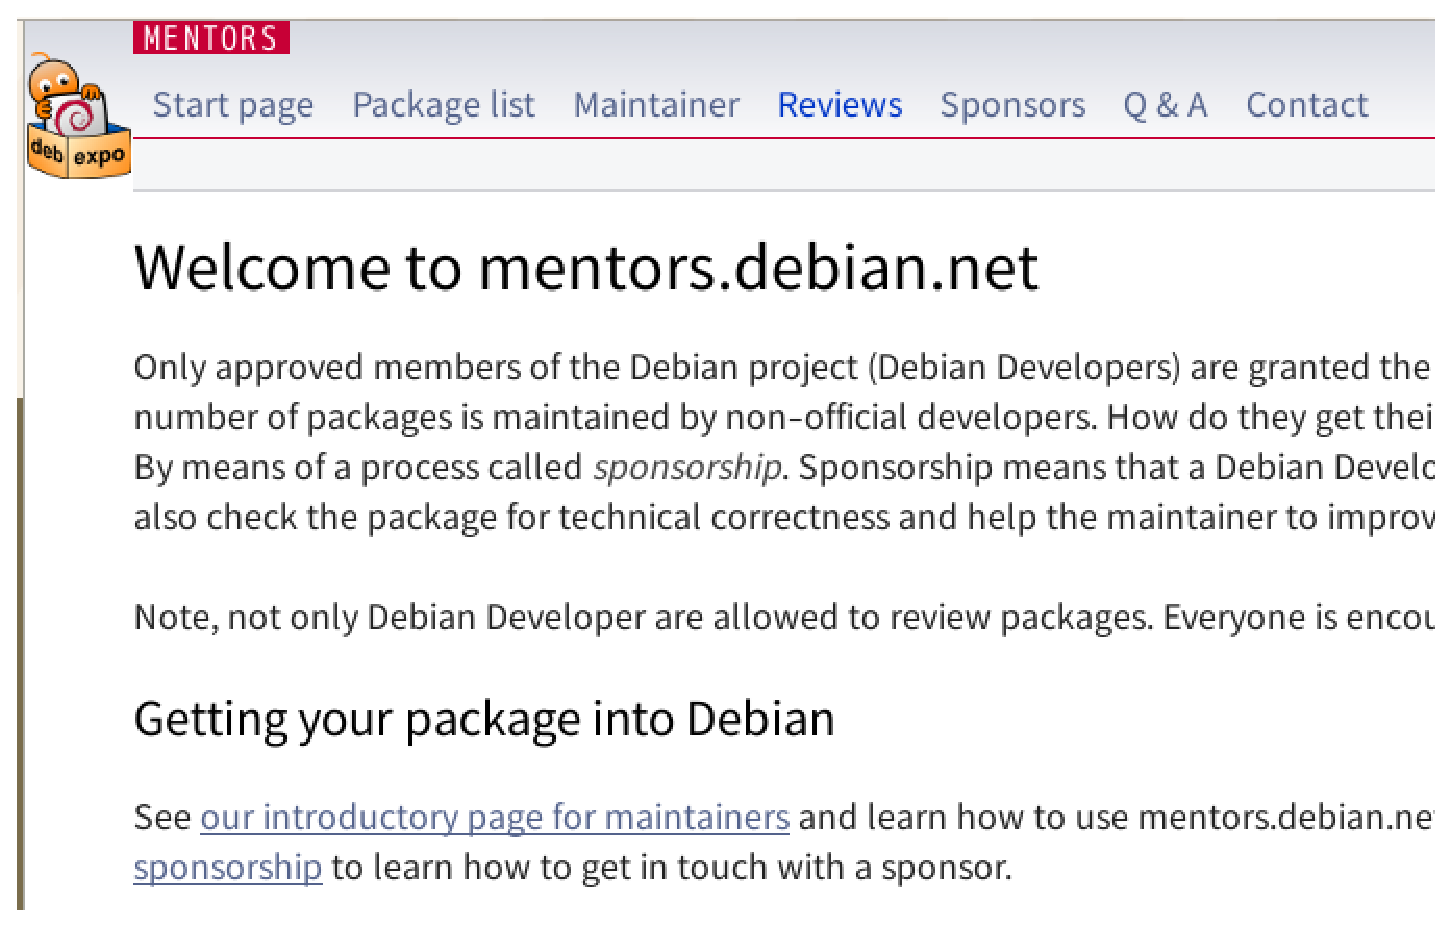
\includegraphics[width=0.5\hsize]{image201606/mentors.d.n.eps}
\end{center}

debexpo$B$N8x<0%5%$%H$O(B\url{https://alioth.debian.org/projects/debexpo/}$B$G$9!#(B
$B0JA03+H/$NCf?4$H$J$C$F$$$?%5%$%H(B\url{https://workaround.org/project/debexpo}$B$K$O(Bdebexpo$B$NL>A0$NM3Mh$,<!$N$h$&$K5-:\$5$l$F$$$^$9!#(B

\begin{quotation}
The new project was called "debexpo" because it was supposed to become an {\color{red}expo}sition for {\color{red}Deb}ian packages.
\end{quotation}

$B%Q%C%1!<%8$,0lF1$K2q$9$kE8Mw2q$H$G$b$$$C$?$H$3$m$G$7$g$&$+!#(B

\subsubsection{debexpo$B35MW(B}

debexpo$B$N0LCVIU$1$,$I$&$$$&$b$N$+$J$s$H$J$/$o$+$C$?$H$3$m$G!"$b$&$9$3$76qBNE*$J>R2p$r$7$^$7$g$&!#(B

debexpo$B$NFCD'$r$$$/$D$+>R2p$9$k$H0J2<$,$"$2$i$l$^$9!#(B

\begin{itemize}
\item Python$B@=(B
\item Pylons\footnote{\url{http://www.pylonsproject.org/}}$B%U%l!<%`%o!<%/:NMQ(B
\item $B%F%s%W%l!<%H%(%s%8%s$O(BMako\footnote{\url{}}
\end{itemize}

$B$3$N(BPylons$B$H$$$&%U%l!<%`%o!<%/!"$"$^$jCN$i$J$$?M$,$$$k$+$bCN$l$^$;$s$N$GJdB-$7$F$*$/$H!"(B

\begin{itemize}
\item Rails$B$C$]$$%U%l!<%`%o!<%/(B
\item 2011$BG/$K%a%s%F%J%s%9%b!<%IF~$j$7$?8O$l$?%U%l!<%`%o!<%/$G$9(B
\item $B8e7Q$H$7$F(BPyramid$B$H$$$&%U%l!<%`%o!<%/$,3+H/$5$l$F$$$^$9(B
\end{itemize}

$B$H$$$&FCD'$,$"$j$^$9!#(B

\begin{itembox}[l]{$B%3%i%`!'(Bdebexpo$B$K$b$f$k%-%c%i$,!)(B}

\includegraphics[width=0.2\hsize]{image201606/debexpo-mascot-zoom.eps}
debexpo$B$K$O!"<B$O$f$k%-%c%i$,@_Dj$5$l$F$$$^$9!#(BWeb$B%5%$%H$N:8>e6y$N@VOH$G0O$C$F$$$k$H$3$m$K2?$+$$$^$9$h$M!"$=$l$G$9!#(B
$B$?$@$7!">\:Y$OITL@$G$9!#(BSUUMO\footnote{$BITF0;:>pJs%5%$%H!#(B\url{http://suumo.jp/}}$B$N%9!<%b(B\footnote{$B%^%9%3%C%H%-%c%i%/%?!<!#%9!<%b$NIt20(B\url{http://suumo.jp/edit/suumo-heya/}$B$H$$$&FC@_%Z!<%8$,$"$k!#(B}$B$K$OJR;W$$$N%9%b%_$H$NA[A|>e$N;R6!%9%b%k$,$$$k$H$$$&@_Dj(B\footnote{\url{http://suumo.jp/edit/suumo-heya/character/suumo_character.pdf}}
$B$,$"$k$/$i$$$J$N$G!"$3$N%-%c%i$K$b2?$+$"$j$=$&$J5$$b$7$^$9$,!#!#!#(B
\end{itembox}

\subsection{$B$J$<(Bdebexpo$B$r%O%C%/$9$kI,MW$,!)(B}

$B%Q%C%1!<%8$r%9%]%s%5!<$7$F$b$i$&$H$-$K;H$&(Bmentors.d.n$B$K$O$$$/$D$+$*A&$a$JE@$,$"$j$^$9!#(B

\begin{itemize}
  \item $B%Q%C%1!<%8$N%A%'%C%/$b$7$F$/$l$k(B
  \item RFS$B$N%F%s%W%l!<%H$b@8@.$7$F$/$l$k(B
\end{itemize}

\begin{screen}
  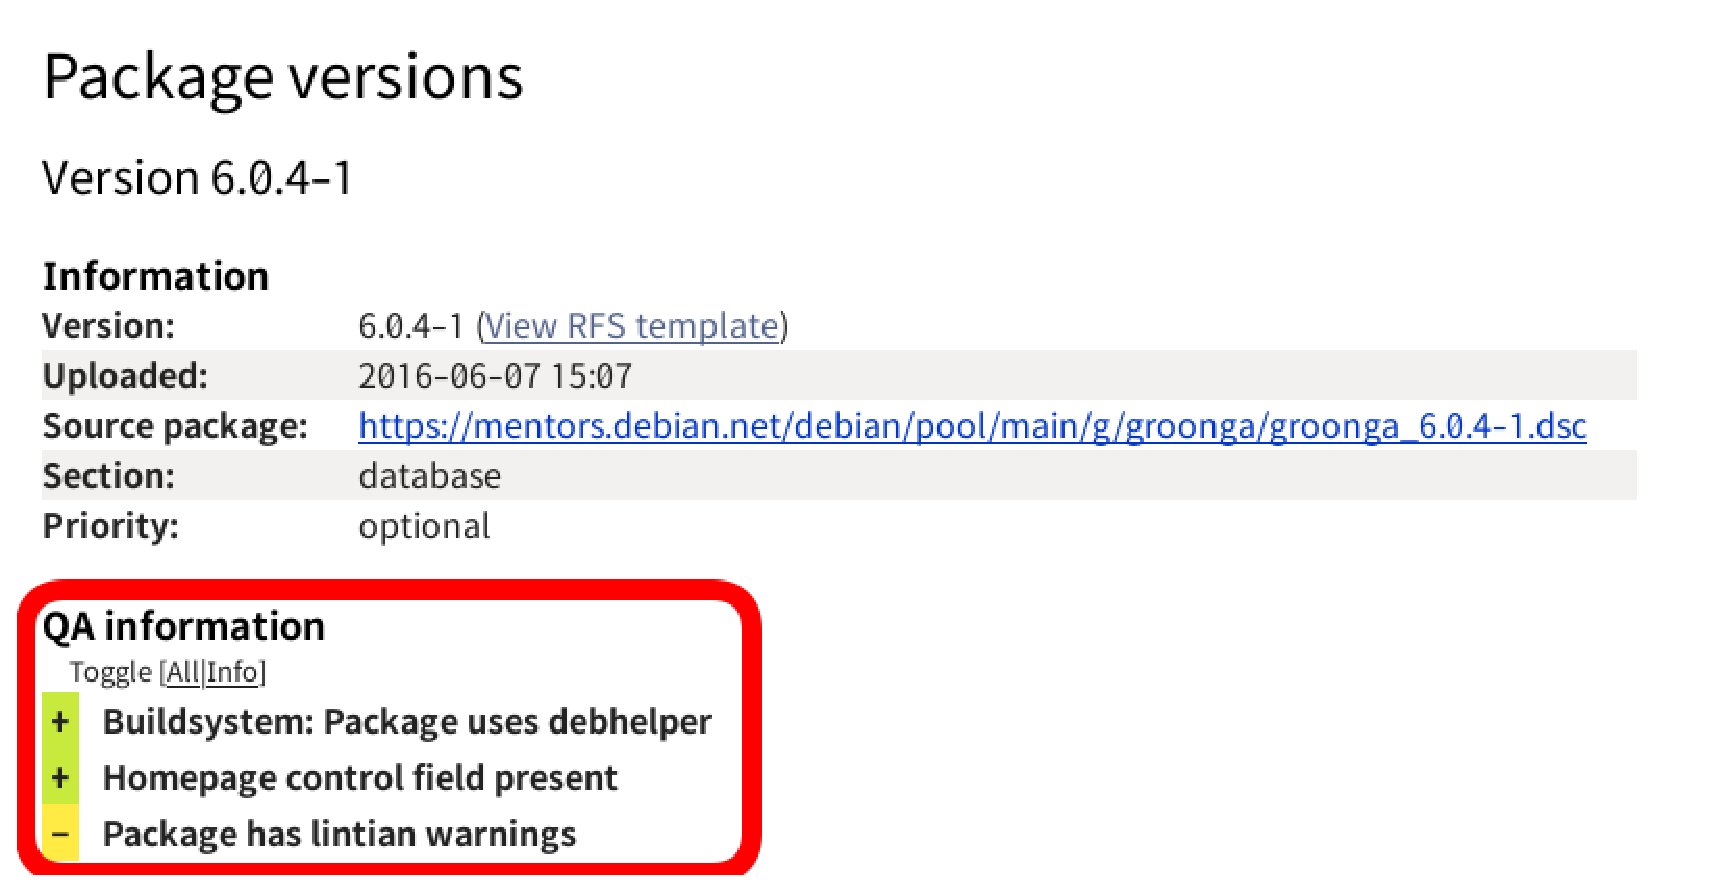
\includegraphics[width=0.8\hsize]{image201606/qa-information.eps}
\end{screen}

$B%9%/%j!<%s%7%g%C%H$+$i$b$o$+$k$h$&$K!"(BQA information$B$NMs$K(BLintian$B$N7Y9p$J$I$,I=<($5$l$k$h$&$K$J$C$F$$$^$9!#(B

\begin{screen}
  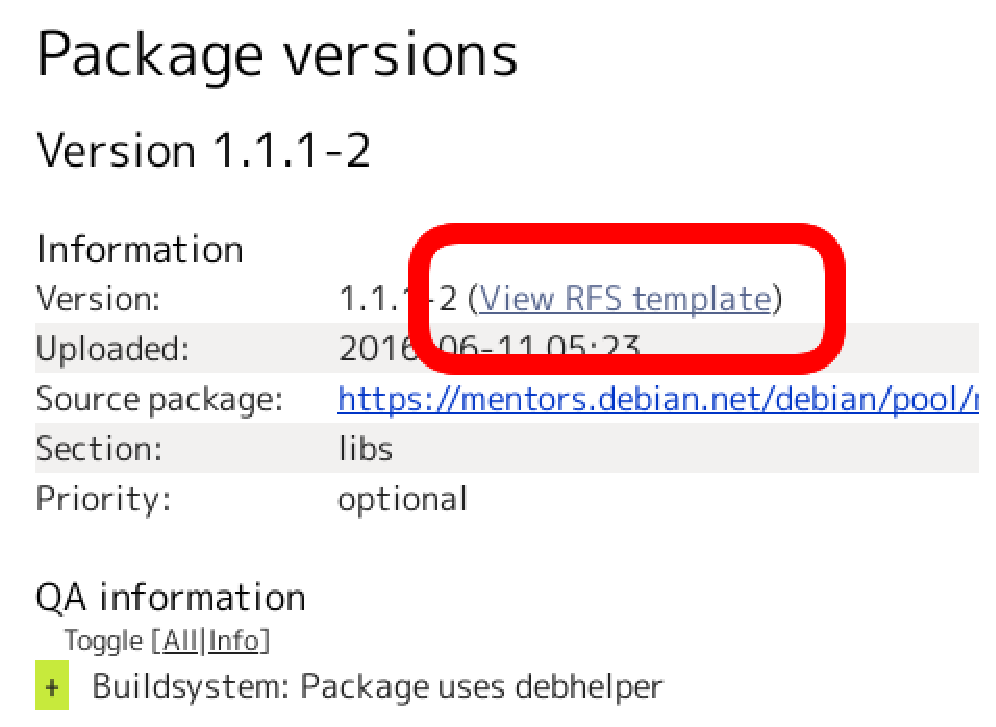
\includegraphics[width=0.5\hsize]{image201606/view-rfs-template.eps}
\end{screen}

$B$^$?!"%9%/%j!<%s%7%g%C%H$N!V(BView RFS template$B!W$N%j%s%/$r$?$I$k$H!"(BRFS$B$N%F%s%W%l!<%H$b@8@.$7$F$/$l$k$H$$$&$N$b4r$7$$%]%$%s%H$G$9!#(B

$B$J$N$G!"$"$H$O$3$N(BRFS$B%F%s%W%l!<%H$r$b$H$K$7$F!"%a!<%k$9$k$@$1$K$J$C$F$$$^$9!#(B\footnote{$B$H$O$$$&$b$N$N!"13$G$O$J$$$,!"@53N$G$b$J$$!#(B}

$B<B:]$N(BRFS template$B$r8+$F$_$^$7$g$&!#(B

\begin{screen}
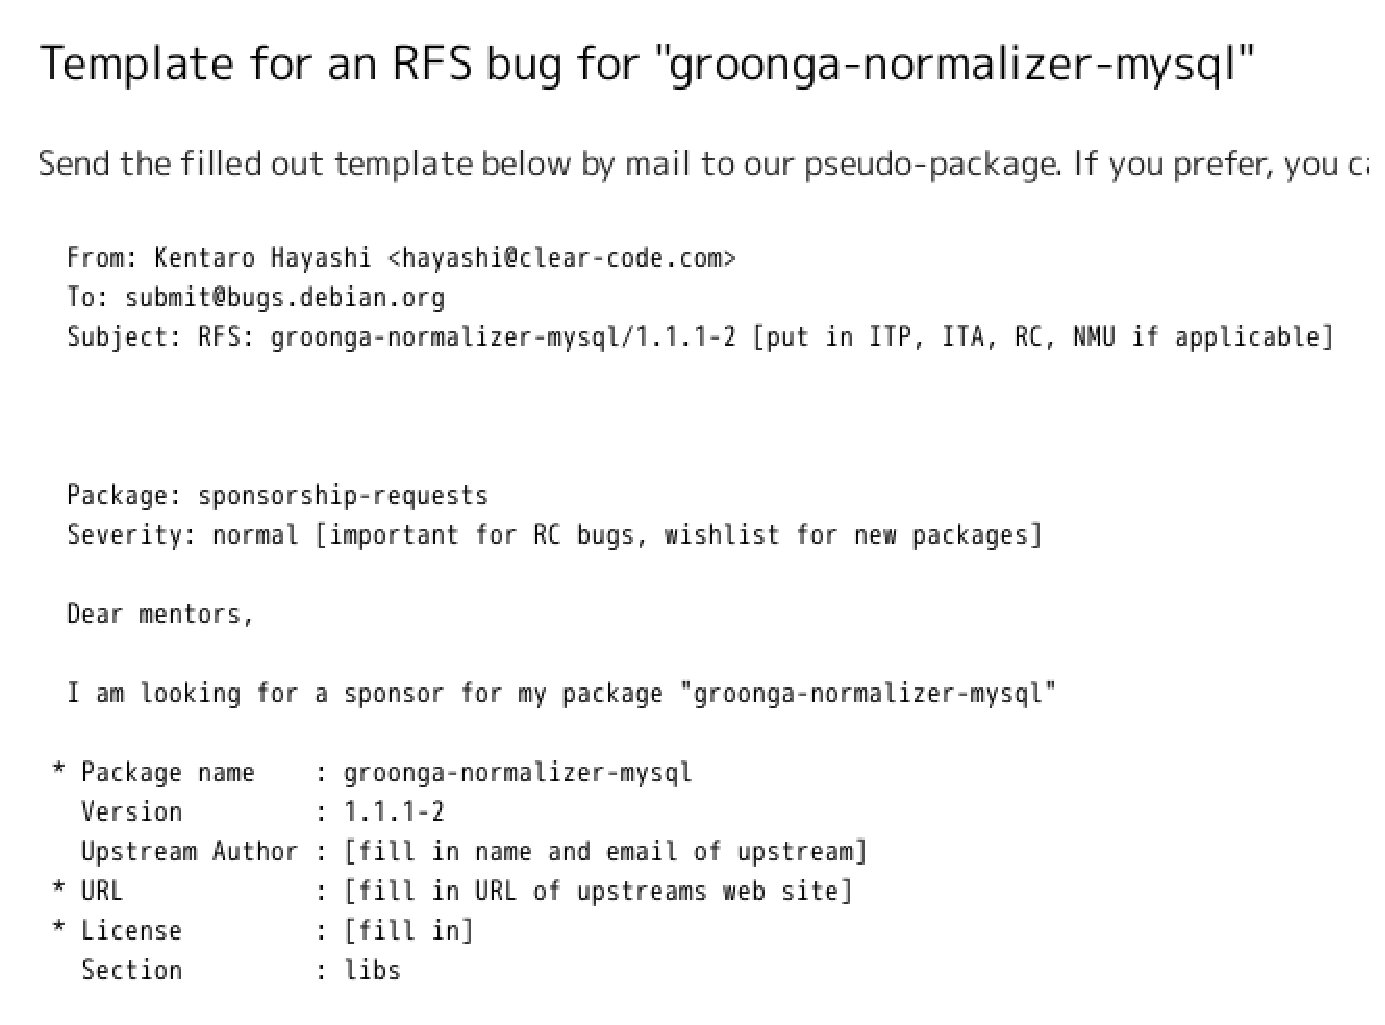
\includegraphics[width=0.5\hsize]{image201606/rfs-template-pithole.eps}
\end{screen}

[fill in]$B$NJ8;z$,$A$i$[$i$"$k$N$,$o$+$j$^$9$M!#(B

\begin{screen}
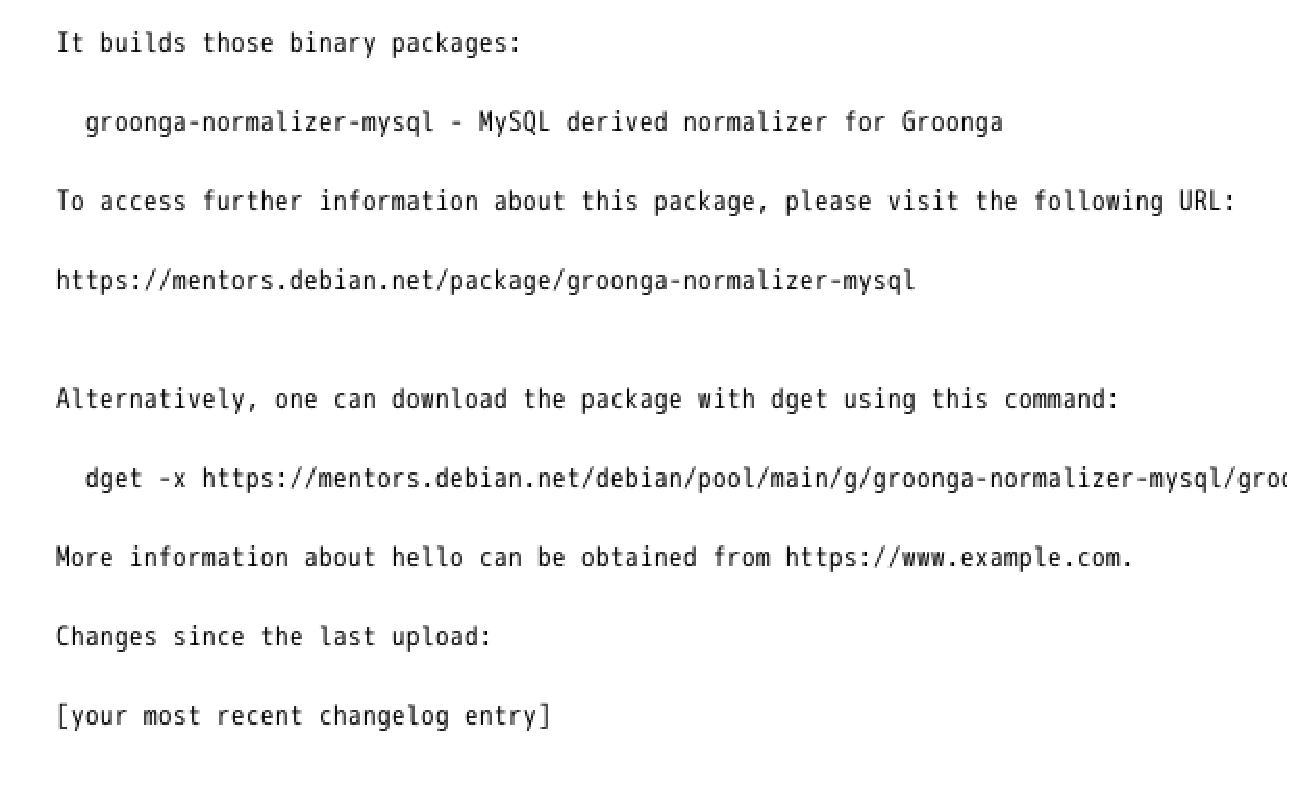
\includegraphics[width=0.5\hsize]{image201606/rfs-template-pithole2.eps}
\end{screen}

$B$3$l$@$1$G$O$"$j$^$;$s!#$[$+$K$b7jKd$a$,I,MW$G$9!#(B

\begin{screen}
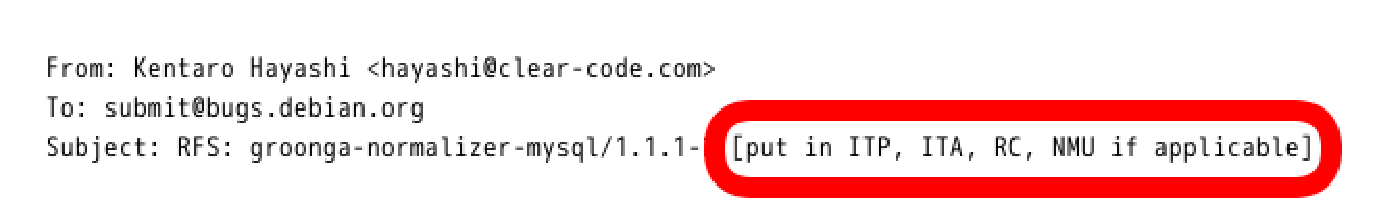
\includegraphics[width=0.5\hsize]{image201606/rfs-template-fill-in1.eps}
\end{screen}

Subject:$B$K<oJL$r=q$+$J$$$H$$$1$^$;$s!#(B

\begin{screen}
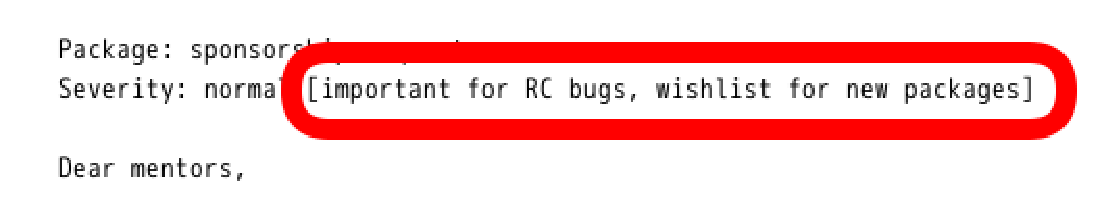
\includegraphics[width=0.5\hsize]{image201606/rfs-template-fill-in2.eps}
\end{screen}

Severity:$B$r=q$+$J$$$H$$$1$^$;$s!#(B

\begin{screen}
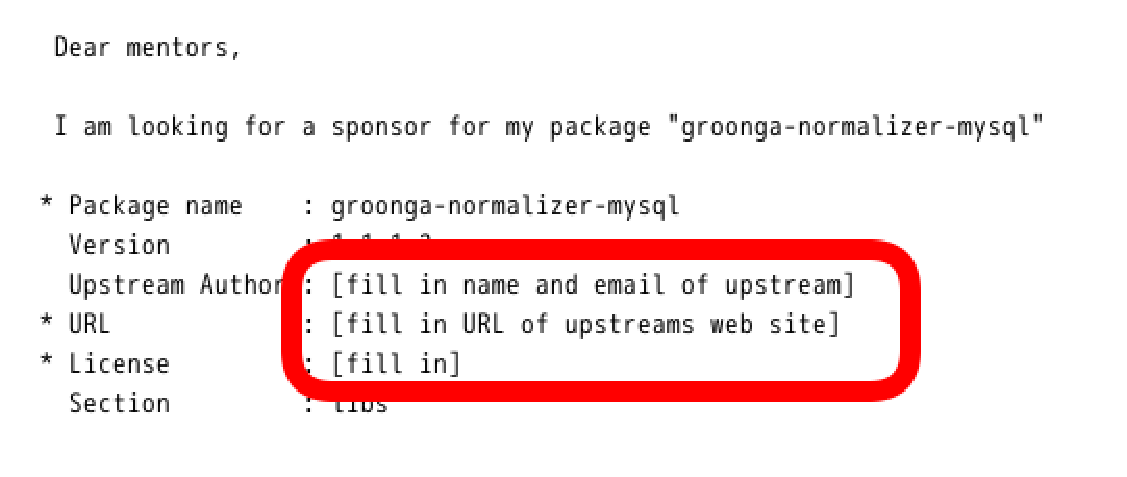
\includegraphics[width=0.5\hsize]{image201606/rfs-template-fill-in3.eps}
\end{screen}

Upstream,URL,License:$B$r=q$+$J$$$H$$$1$^$;$s!#(B

\begin{screen}
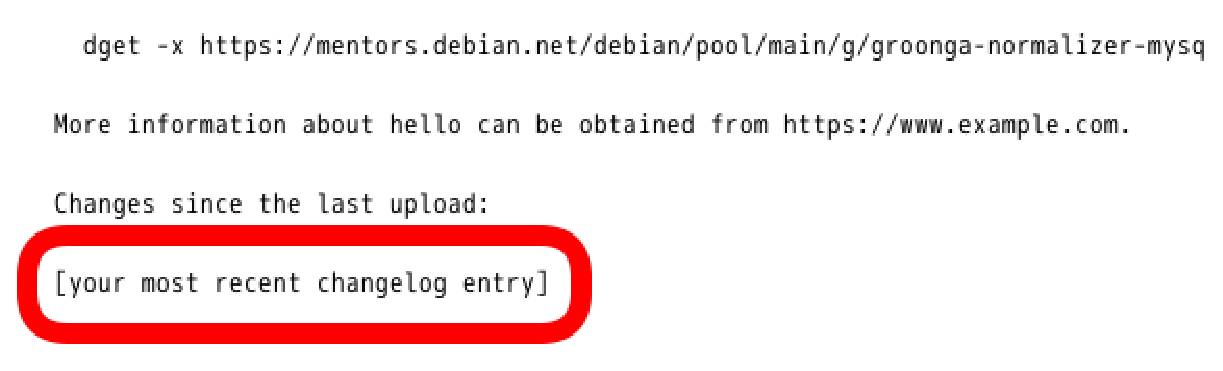
\includegraphics[width=0.5\hsize]{image201606/rfs-template-fill-in4.eps}
\end{screen}

Changelog$B$r=q$+$J$$$H$$$1$^$;$s!#(B

$B$3$l$G=*$o$j$G$7$g$&$+!#$$$$$(0c$$$^$9!#(B

\begin{screen}
\includegraphics[width=0.5\hsize]{image201606/rfs-template-fill-in5.eps}
\end{screen}

$B$5$j$2$J$/Kd$a$3$^$l$?(Bhello$B$H(Bexample.com$B$,;D$C$F$$$^$9!#(B

$B$h$&$d$/$"$l$3$lD>$7=*$($^$7$?!#$3$l$G%a!<%k$,=P$;$k$H!";W$&$+$bCN$l$^$;$s!#;v<B;d$b:G=i$O$=$&;W$$$^$7$?!#(B

$B$3$3$GLdBj$K$J$k$N$,!"@hF,$KKd$a$3$^$l$?%9%Z!<%9(B2$B$D$G$9!#(B

\begin{screen}
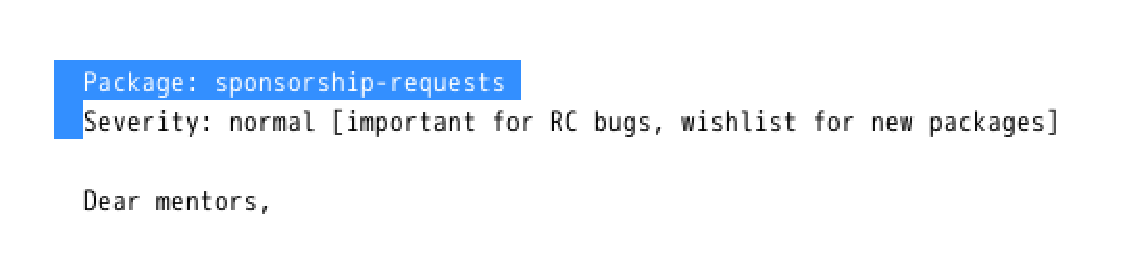
\includegraphics[width=0.5\hsize]{image201606/rfs-template-pithole3.eps}
\end{screen}

$B$3$3$G!">e5-$O%3%^%s%I%a!<%k$G$"$k$3$H$r;W$$$@$5$M$P$J$j$^$;$s!#$D$^$j!"$=$N$^$^%a!<%k$9$k$H$b$A$m$s%(%i!<$K$J$j$^$9!#(B

$B$7$?$,$C$F!"!V$J$<(Bdebexpo$B$r%O%C%/$9$k$N$+!)!W$KBP$9$kEz$($O!"!V(BRFS$B%F%s%W%l!<%H$N;DG0$C$W$j$r$I$&$K$+$7$?$$!W$+$i!"$H$$$&$3$H$K$J$j$^$9!#(B

\begin{screen}
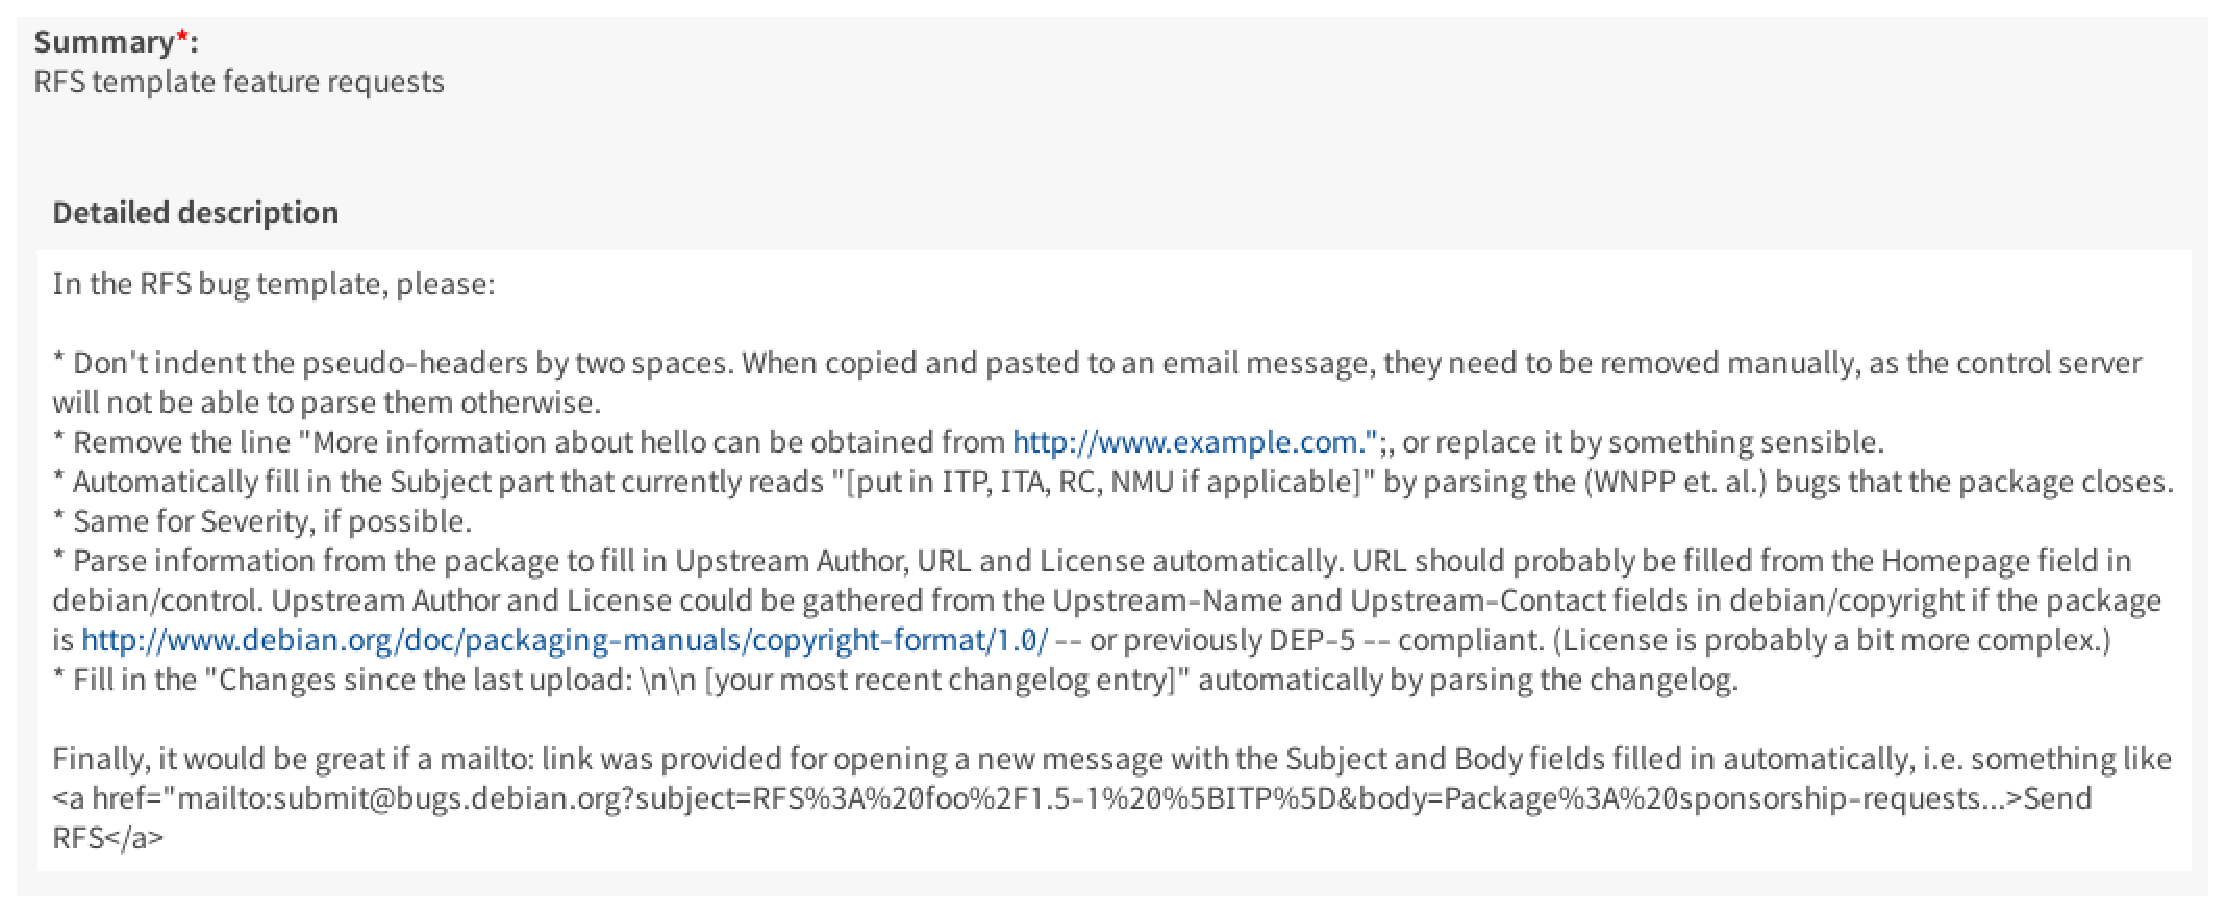
\includegraphics[width=1.0\hsize]{image201606/alioth-debexpo-313593-request.eps}
\end{screen}

Alioth$B$r$_$F$_$k$H!"F1$8;W$$$N?M$,$$$^$7$?!#$=$l$O(BAlioth$B$N(Btracker$B$G(B4$BG/$bA0$KDL$C$?F;$@!"$H$$$&!#(B

\subsection{$B$I$&$d$C$F%O%C%/$7$?$N$+!)(B}

$B$*$*$`$M!"0J2<$NN.$l$G(Bdebexpo$B$r%O%C%/$9$k$3$H$K$J$j$^$7$?!#(B

\begin{itemize}
  \item upstream$BC5$7(B
  \item $B%I%-%e%a%s%HC5$7(B
  \item $B$^$:$OF0$+$7$F$_$k(B
  \item $B$"$?$j$r$D$1$F=$@5(B
  \item $B$=$7$F(BPR$B$X(B
\end{itemize}

$BFCJL$J$3$H$O2?$b$J$/$F!"$h$/$"$k%U%j!<%=%U%H%&%'%"$N=$@5$G$9!#(B

\begin{itembox}[l]{$B%3%i%`!'(Bdebexpo$B$NNr;K$K$D$$$F(B}
debexpo$B$O(B2003$BG/$K:G=i$N%3!<%I$,(BPerl$B$G=q$+$l$^$7$?!#$7$+$7!"5!G=3HD%$NMWK>$K1~$($?$j$7$F$$$/$K$O;Y>c$,$"$C$?$?$a!"(BPython$B$G=q$-D>$5$l$?$H$$$&7P0^$,$"$j$^$9!#(B
debexpo$B$N3+H/$,3hH/$K$J$C$?$N$O!"(B2008$BG/$N$3$H$G$9!#(BGoogle SoC$B$K:NBr$5$l$?$?$a!"(BJonny Lamb$B;a$i$K$h$j0l5$$K3+H/$,$9$9$_$^$7$?!#(B

2009$BG/$+$i(B2010$BG/$O$f$k$d$+$J3+H/$,B3$-$^$7$?!#(Bhttp://expo.debian.net/$B$,8x3+$5$l$?$N$b$3$N$3$m$G$9!#8=:_$N(Bmentors.d.n$B$X$H@Z$jBX$($i$l$?$N$O(B2011$BG/$N$3$H$G$9!#(B
$B$=$N8e$b!"(B2012$BG/$K$O(BUI$B$N2~A1(B(debexpo v2)$B$d:FEY(BGSoC$B$X$N:NBr(B(debexpo v3)$B$J$I$H3+H/$,B3$$$F$$$^$9!#(B

$B$3$N$"$?$j$NJQA+$K$D$$$F!"(BNicolas Dandrimont$B;a$K$h$k!V(BThe State of mentors.debian.net GSOC and Beyond$B!W$H$$$&H/I=;qNA$K>\$7$/=q$+$l$F$$$k$N$G6=L#$,$"$k?M$O;2>H$9$k$H$h$$$G$7$g$&!#(B
\footnote{\url{http://fr2012.mini.debconf.org/slides/debexpo.pdf}}
\end{itembox}

\subsubsection{upstream$BC5$7(B}

\begin{screen}
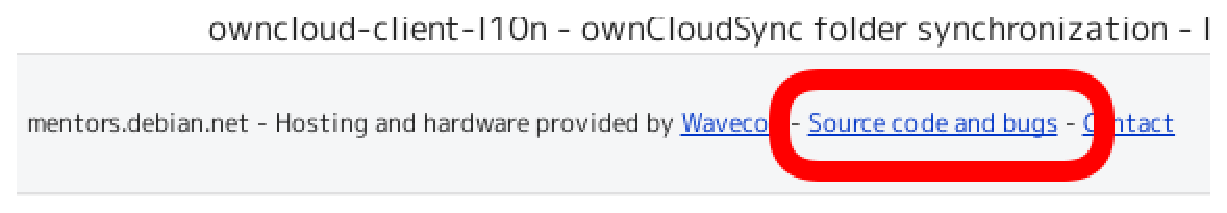
\includegraphics[width=0.5\hsize]{image201606/source-code-and-bugs.eps}
\end{screen}

debexpo$B$N>l9g$K$O!"(Bmentors.d.n$B2<It$K%j%s%/$,$-$A$s$H$"$k$N$G!"(BAlioth$B$r$_$l$P$$$$$H$o$+$j$^$7$?!#(B

\begin{screen}
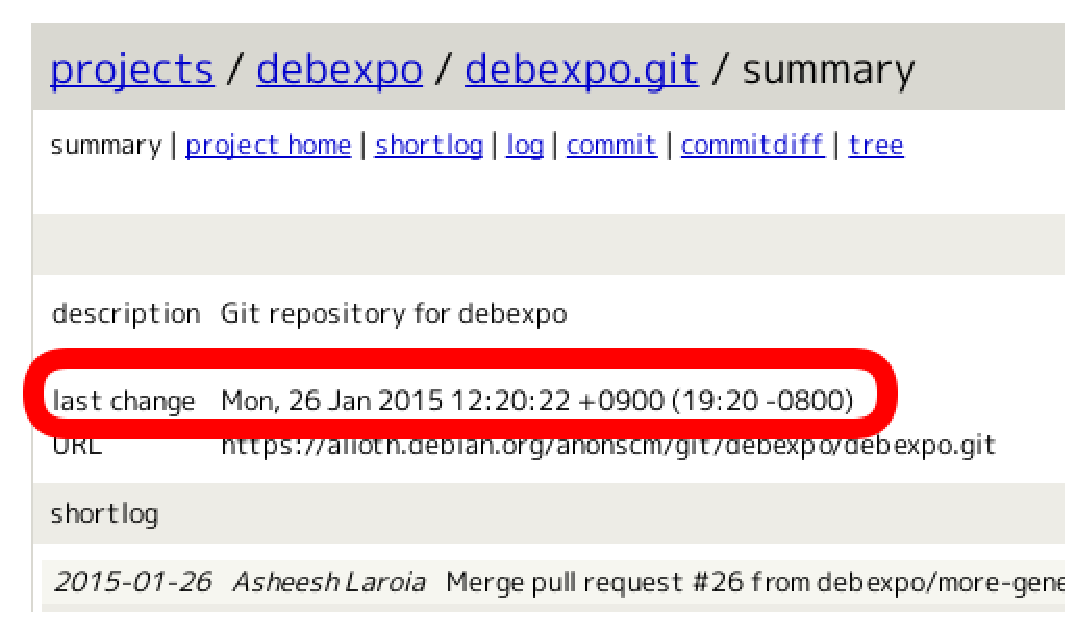
\includegraphics[width=0.5\hsize]{image201606/last-change-on-alioth.eps}
\end{screen}

$B$?$@!"$I$&$d$i:G6a$O%3%_%C%H$,$J$$$N$,IT0B$K$J$j$^$7$?!#(B
$B$h$/;H$o$l$F$$$k$J$i$=$3$=$3%a%s%F$5$l$F$$$k%$%a!<%8$,$"$C$?$+$i$G$9!#<B:]$K$O$=$&$G$b$"$j$^$;$s$G$7$?!#(B

\begin{screen}
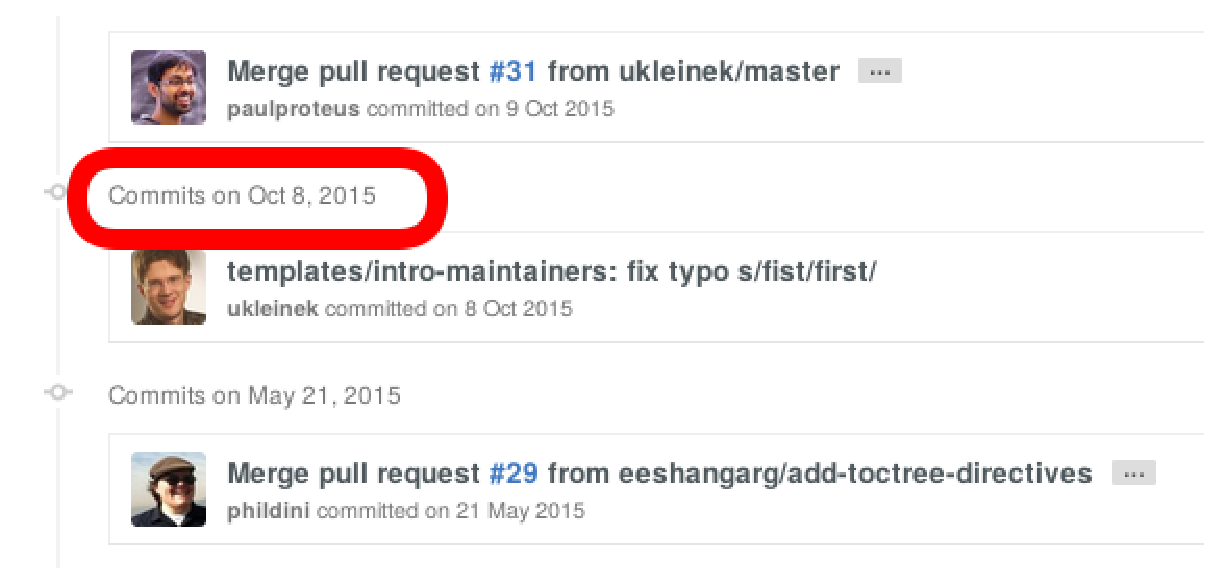
\includegraphics[width=0.7\hsize]{image201606/last-change-on-github.eps}
\end{screen}

$B$"$H$+$i!"(BGitHub$B$N$[$&$,<B$O?7$7$$(B\footnote{\url{https://github.com/debexpo/debexpo}}$B$3$H$,$o$+$j$^$7$?!#(B

$B<B:]$N1?MQ$H$7$F$O!"(BAlioth$B$,(Bmaster\url{https://alioth.debian.org/projects/debexpo/}$B$G!"(BGitHub$B$N$r%^!<%8$H$$$&1?MQ$K$J$C$F$$$k$h$&$G$9!#(B

\subsubsection{$B%I%-%e%a%s%HC5$7(B}

$B%j%]%8%H%j$N(Bdocs/*$B$K%I%-%e%a%s%H$,@0Hw$5$l$F$$$^$7$?!#%$%s%9%H!<%k<j=g$O(Bdocs/installing.rst$B$r;2>H$9$l$P$h$$$H$o$+$j$^$7$?!#(B
$B$?$@!";DG0$J$3$H$K$=$NFbMF$N0lIt$O%j%s%/@h$,(B404$B$K$J$C$F$7$^$C$F$$$^$7$?!#(B

\subsubsection{$B$^$:$OF0$+$7$F$_$k(B}

$B%I%-%e%a%s%H$+$i!"%;%C%H%"%C%WJ}K!$O(B3$B<oN`$"$k$3$H$,$o$+$j$^$7$?!#(B

\begin{itemize}
  \item $B4{B8%7%9%F%`$K%$%s%9%H!<%k(B
  \item virtualenv$B$G%$%s%9%H!<%k(B
  \item VirtualBox$B$G%$%s%9%H!<%k(B
\end{itemize}

$B$^$:$O(BVirtualBox$B$G;n$7$F$_$k$3$H$K$7$^$7$?!#4D6-$rJ,$1$?$$$N$,$=$NA*BrM}M3$G$9!#(B
$B$?$@!"(BVagrantfile$B$,%"%l$J>uBV$G$"$k$3$H$,$o$+$j$^$7$?!#(B

\begin{screen}
\begin{minted}{sh}
# Every Vagrant virtual environment requires a box to build off of.
config.vm.box = "chef/debian-7.6"
\end{minted}
\end{screen}

Debian 7.6 (2014$BG/(B7$B7n(B12$BF|(B)$B!)$K$J$C$F$$$^$7$?!#(BDebian 7.10$B$,$b$&$9$G$K$G$F$$$k$4;~@$$K$b4X$o$i$:$G$9!#(B

vagrant up$B$7$F$_$k$H$^$?;DG0$J>uBV$G$7$?!#(B

\begin{commandline}
$ vagrant up
Bringing machine 'default' up with 'virtualbox' provider...
==> default: Box 'chef/debian-7.6' could not be found. Attempting to find and install...
  default: Box Provider: virtualbox
  default: Box Version: >= 0
The box 'chef/debian-7.6' could not be found or
could not be accessed in the remote catalog. If this is a private
box on HashiCorp's Atlas, please verify you're logged in via
`vagrant login`. Also, please double-check the name. The expanded
URL and error message are shown below:

URL: ["https://atlas.hashicorp.com/chef/debian-7.6"]
Error: The requested URL returned error: 404 Not Found
}
\end{commandline}

box$B$,8+$D$+$i$J$/$F%3%1$F$$$^$7$?!#$=$3$G!"(BPR\#32$B$G=$@5$7$^$7$?!#(B
$B<:GT$7$F$$$?$N$O!"(BBento project$B$K0\9T$7$F$$$?$;$$$G$7$?!#(B

\begin{screen}
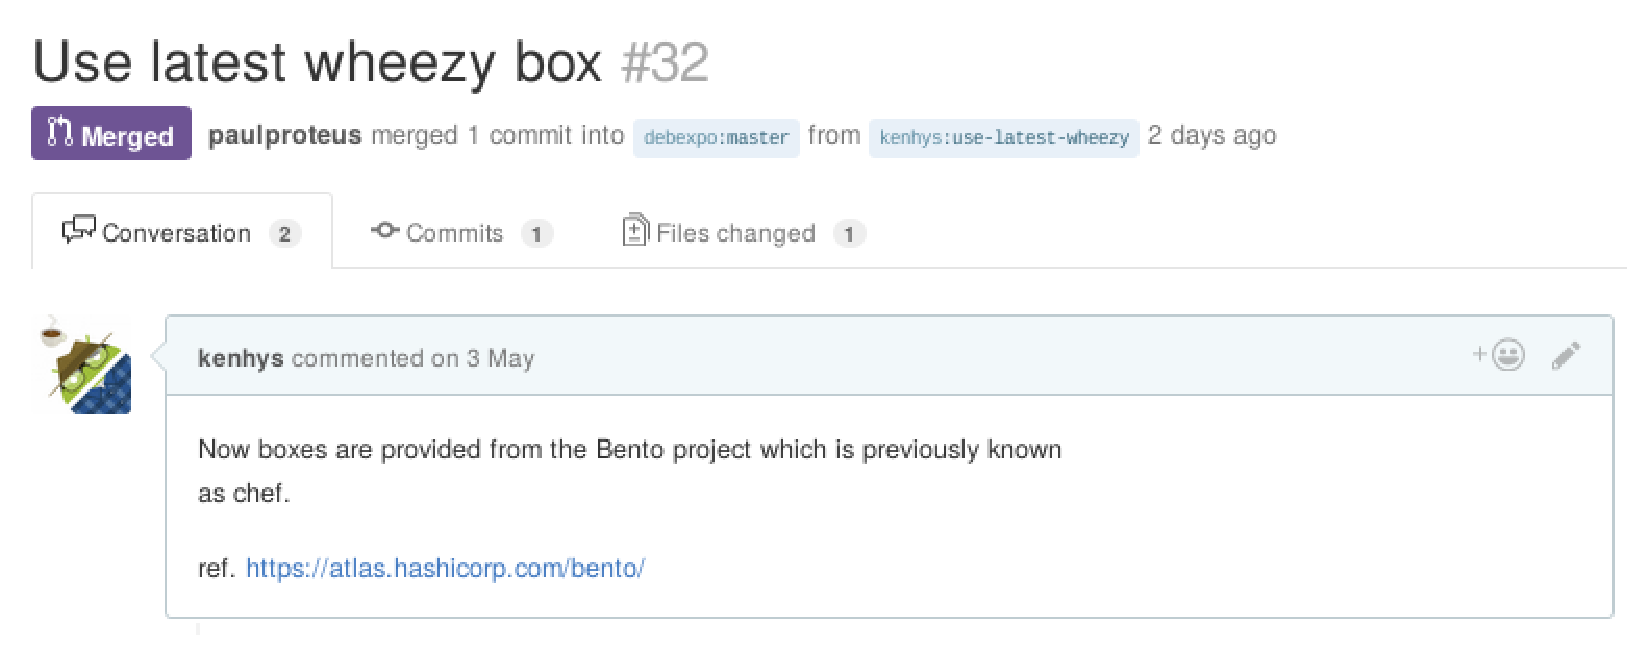
\includegraphics[width=0.7\hsize]{image201606/debexpo-pr32-use-latest-wheezy.eps}
\end{screen}

$B5/F0$7$F!"%m%0%$%s$9$k$K$O<!$N$h$&$K$7$^$9!#(B

\begin{commandline}
$ vagrant up --provision
$ vagrant ssh
\end{commandline}

vagrant ssh$B$7$F(Bpaster$B%3%^%s%I$r<B9T$7$F%5!<%P!<$r5/F0$7$^$9!#(B

\begin{commandline}
$ cd debexpo
$ . venv/bin/activate
$ paster serve development.ini
\end{commandline}

$B$3$N$h$&$K$9$k$H!"(B5000$B%]!<%H$G%5!<%P!<$r5/F0$9$k$3$H$,$G$-$^$9!#(B

\begin{screen}
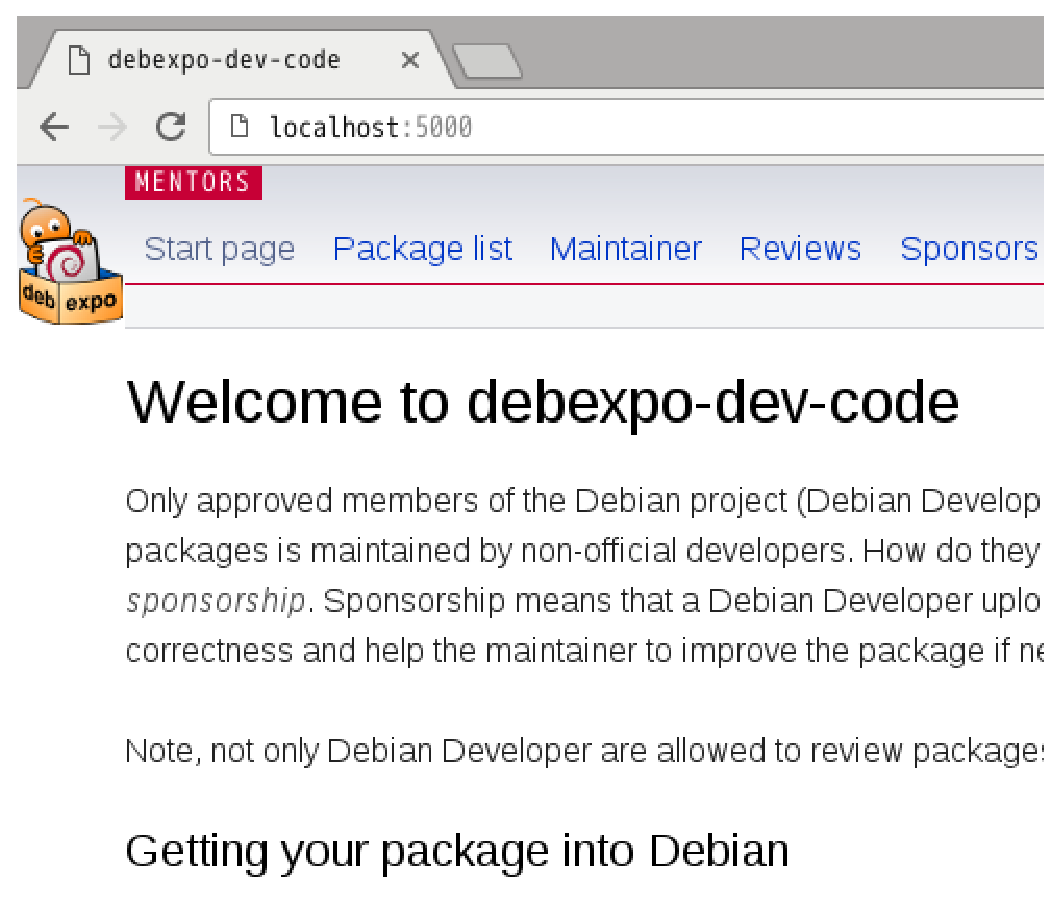
\includegraphics[width=0.5\hsize]{image201606/debexpo-on-localhost.eps}
\end{screen}

$B$3$l$K$h$j%V%i%&%6$G%"%/%;%92DG=$K$J$j$^$9!#(B

$B<!$K%f!<%6!<$NDI2C$r$7$^$9!#J}K!$O(B2$B$D$"$C$F!"%V%i%&%67PM3$GDI2C$9$k$N$H!"(BJSON$B$r$b$H$KDI2C$9$k$d$j$+$?$,$"$j$^$9!#(B

\begin{screen}

\includegraphics[width=0.5\hsize]{image201606/debexpo-sign-me-up.eps}
\end{screen}

JSON$B$GDI2C$9$k$J$i<!$N$h$&$JFbMF$N%U%!%$%k$rMQ0U$7$^$9!#(B

\begin{screen}
\begin{minted}{javascript}
{
  "realname":"Hayashi Kentaro",
  "password":"password",
  "email":"hayashi@clear-code.com"
}
\end{minted}
\end{screen}

$B%f!<%6!<DI2CMQ$N%9%/%j%W%H$,MQ0U$5$l$F$$$k$N$G!"$=$l$rMxMQ$7$^$9!#(B

\begin{commandline}
$ python ./bin/user_importer.py -i development.ini -u user.json
\end{commandline}

$B<!$K%"%+%&%s%H$NM-8z2=$r$7$^$9!#%"%+%&%s%H$rM-8z$K$9$k$K$O(B2$B$D@_Dj$r$9$kI,MW$,$"$j$^$9!#(B

\begin{itemize}
\item verification ($B%m%0%$%s$KI,MW(B)
\item dmup ($B%"%C%W%m!<%I$KI,MW(B)
\end{itemize}

verification$B$N@_Dj$O<!$N$h$&$J%/%(%j$r<B9T$9$k$3$H$G9T$$$^$9!#(B

\begin{screen}

\includegraphics[width=0.7\hsize]{image201606/update-verification.eps}
\end{screen}

verification$B$r6u$K$9$k$3$H$G!"%a!<%k$K$h$k3NG'%W%m%;%9$r1*2s$9$k$3$H$,$G$-$^$9!#(B

$B$b$&0l$D!"(BDMUP$B$H$O%^%7%s;HMQ%]%j%7!<$N$3$H$G$9!#3+H/$G;H$&$@$1$J$N$G!"<!$N$h$&$J%/%(%j$r<B9T$9$k$3$H$G(Bdmup$B%U%#!<%k%I$r99?7$7$F!"F10U$7$?$3$H$K$7$^$9!#(B

\begin{screen}

\includegraphics[width=0.7\hsize]{image201606/update-dmup.eps}
\end{screen}


$B$3$3$^$G$G$-$?$i!"$"$H$O%"%C%W%m!<%I$9$k$?$a$K!"(B.dput.cf$B$N@_Dj$r$7$^$9!#(B

\begin{screen}
\begin{minted}{sh}
[debexpo]
fqdn = localhost:5000
incoming = /upload/kenhys@gmail.com/password
method = http
allow_unsigned_uploads = 0
\end{minted}
\end{screen}

$BMQ0U$G$-$?$i!"<B:]$K%"%C%W%m!<%I$r;n$7$F$_$^$7$g$&!#(B

\begin{commandline}
Uploading to debexpo (via http to localhost:5000):
Uploading groonga_6.0.2-1.dsc:
Upload failed: 500 Internal Server Error
\end{commandline}

$B$H;W$C$?$i!"$"$C$5$j(B500 Internal Server Error$B$KAx6x$7$^$7$?!#(B

\begin{screen}

\includegraphics[width=0.7\hsize]{image201606/find-a-debexpo-bug.eps}
\end{screen}

$B;DG0$J$3$H$K!"$"$k$Y$-%G%#%l%/%H%j$,$J$$$H$$$&%*%A$G$7$?!#(B

$B$=$3$G!"(BPR\#34$B$G=$@5$7$F$H$j$3$s$G$b$i$$$^$7$?!#(B

\begin{screen}
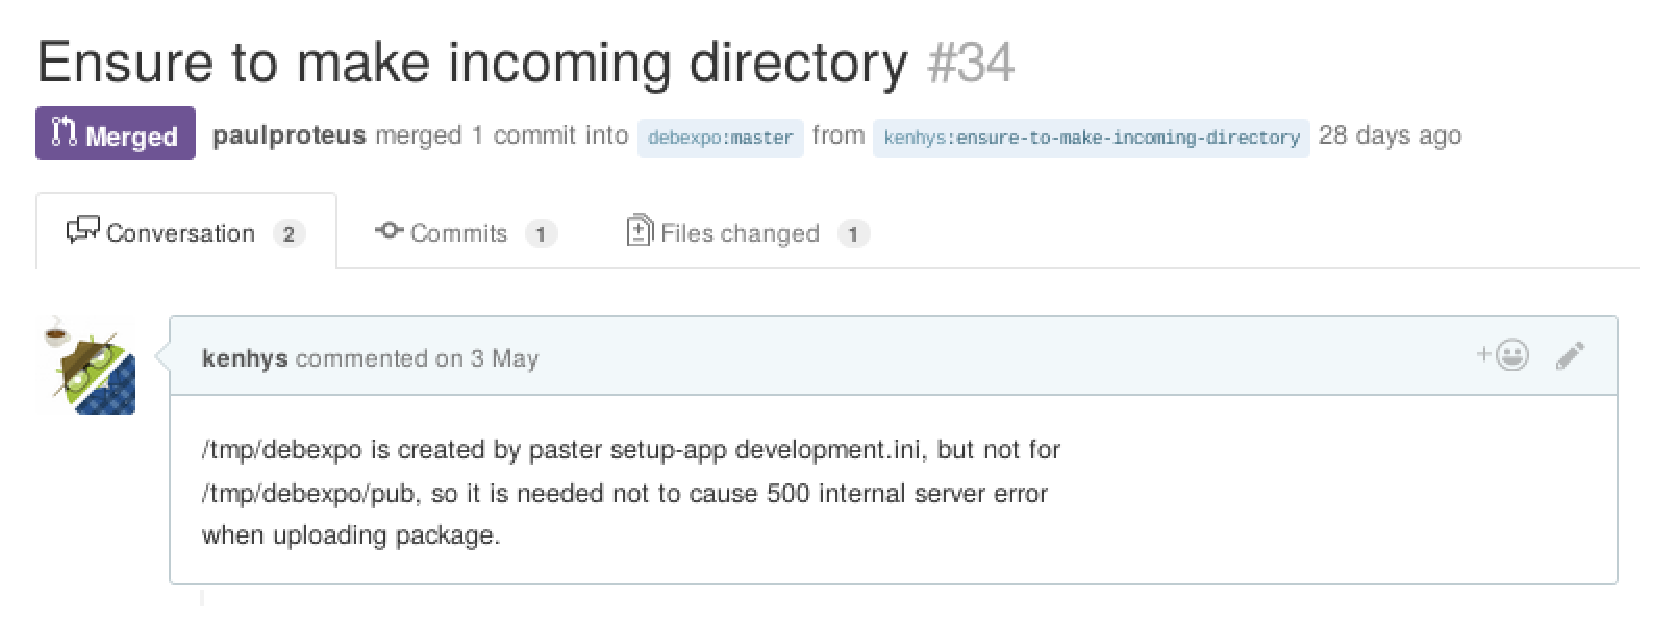
\includegraphics[width=0.7\hsize]{image201606/debexpo-pr34-incoming-directory.eps}
\end{screen}

PR$B$r=P$7$F$_$?$H$-$K5$$E$$$?$N$G$9$,!":G8e$K%F%9%H$,DL$C$?$N(B8$B%v7nA0$H$$$&%*%A$,$D$$$F$$$^$7$?!#(B

\begin{screen}
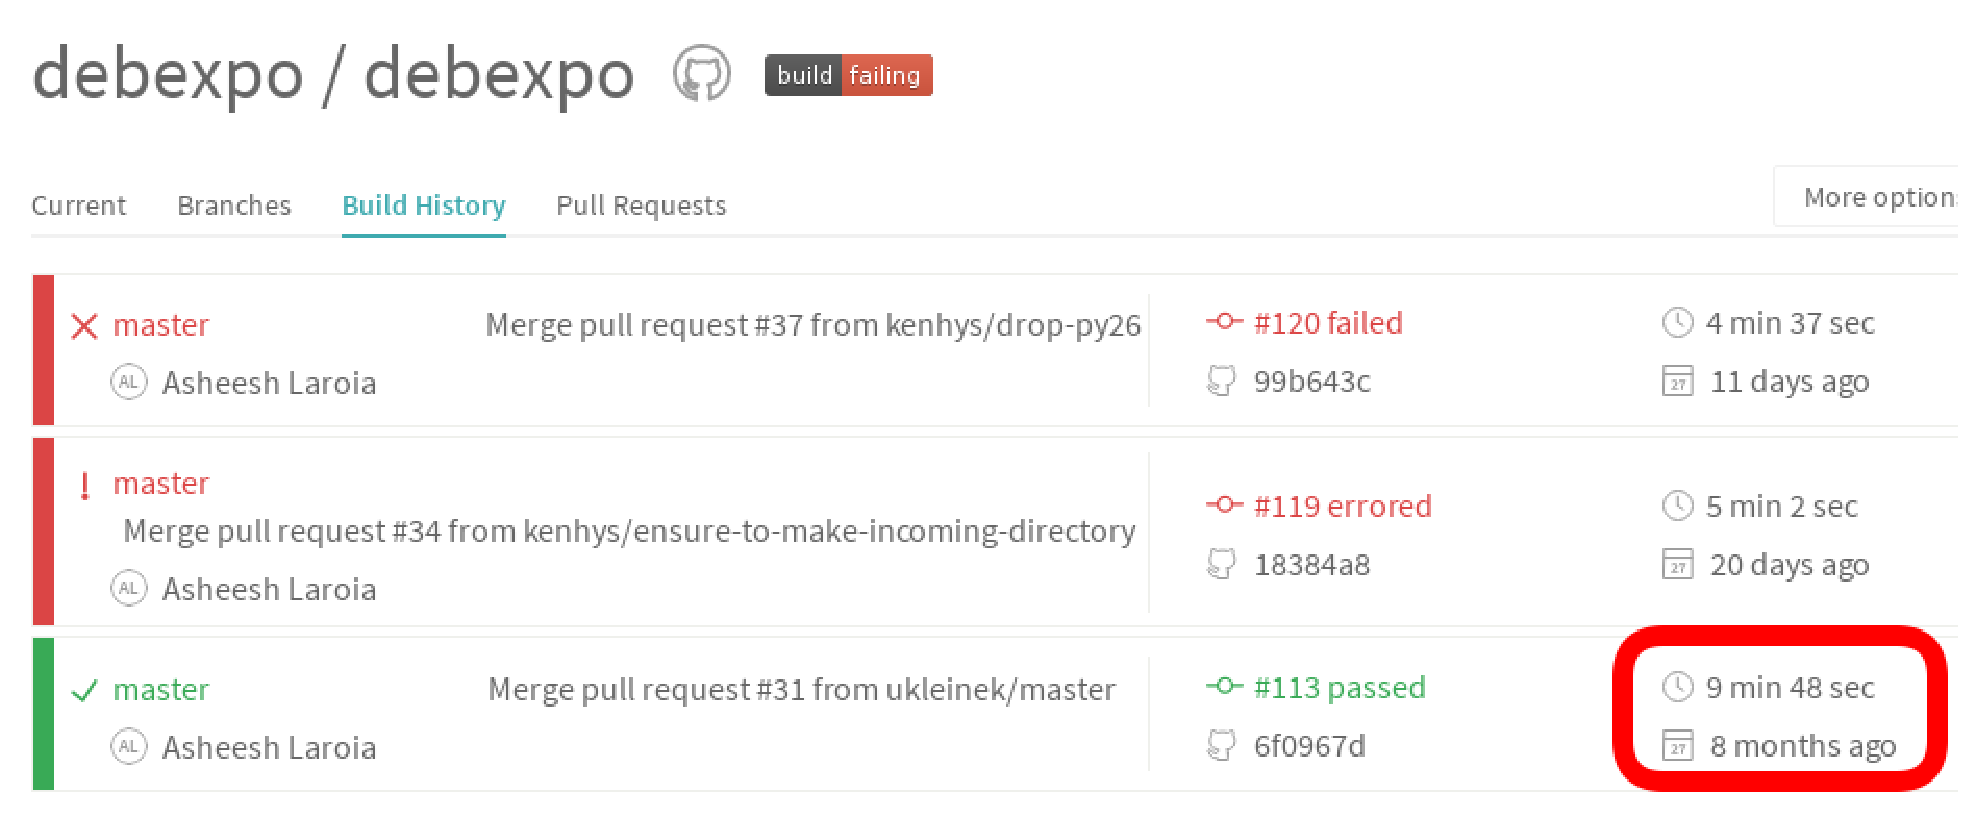
\includegraphics[width=0.7\hsize]{image201606/broken-ci-since-8month-ago.eps}
\end{screen}

$B$3$l$O$J$<$+$H$$$&$H(BTravis-CI$B$N4D6-$NJQ2=$KC/$b5$$$$F$$$J$$>uBV$@$C$?$?$a$G$9!#$7$P$i$/%3%_%C%H$,$J$5$l$F$$$J$$%W%m%8%'%/%H$G$O$"$j$,$A$G$9!#(B
$B$=$3$G!"(BPR\#38$B$G%F%9%H$,DL$k$h$&$K=$@5$7$^$7$?!#(B

\begin{screen}
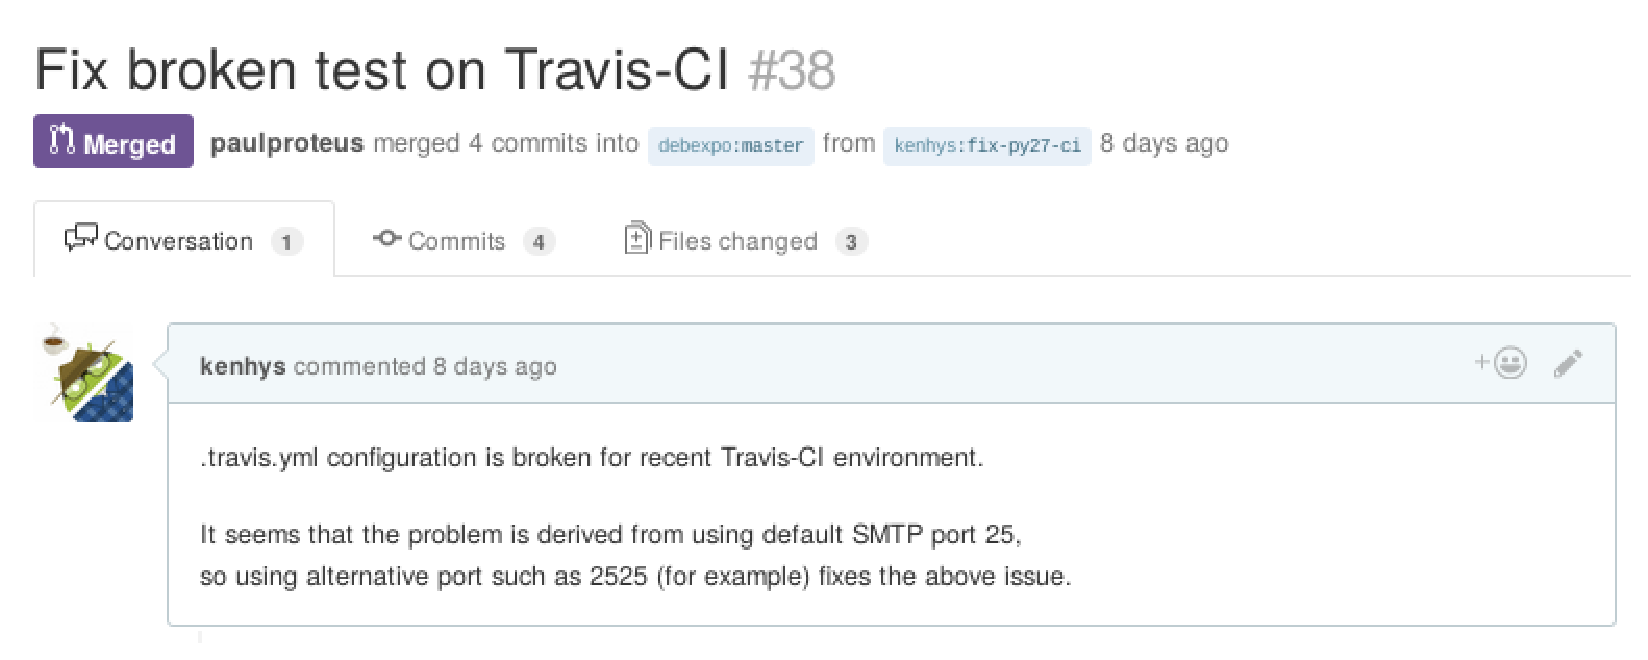
\includegraphics[width=0.7\hsize]{image201606/debexpo-pr38-broken-ci.eps}
\end{screen}

$B$^$?!"(BPython2.6$B$G(BCI$B$O$b$&ITMW$J$N$G!"(BPR\#37$B$G=$@5$b9T$$$^$7$?!#(B

\begin{screen}
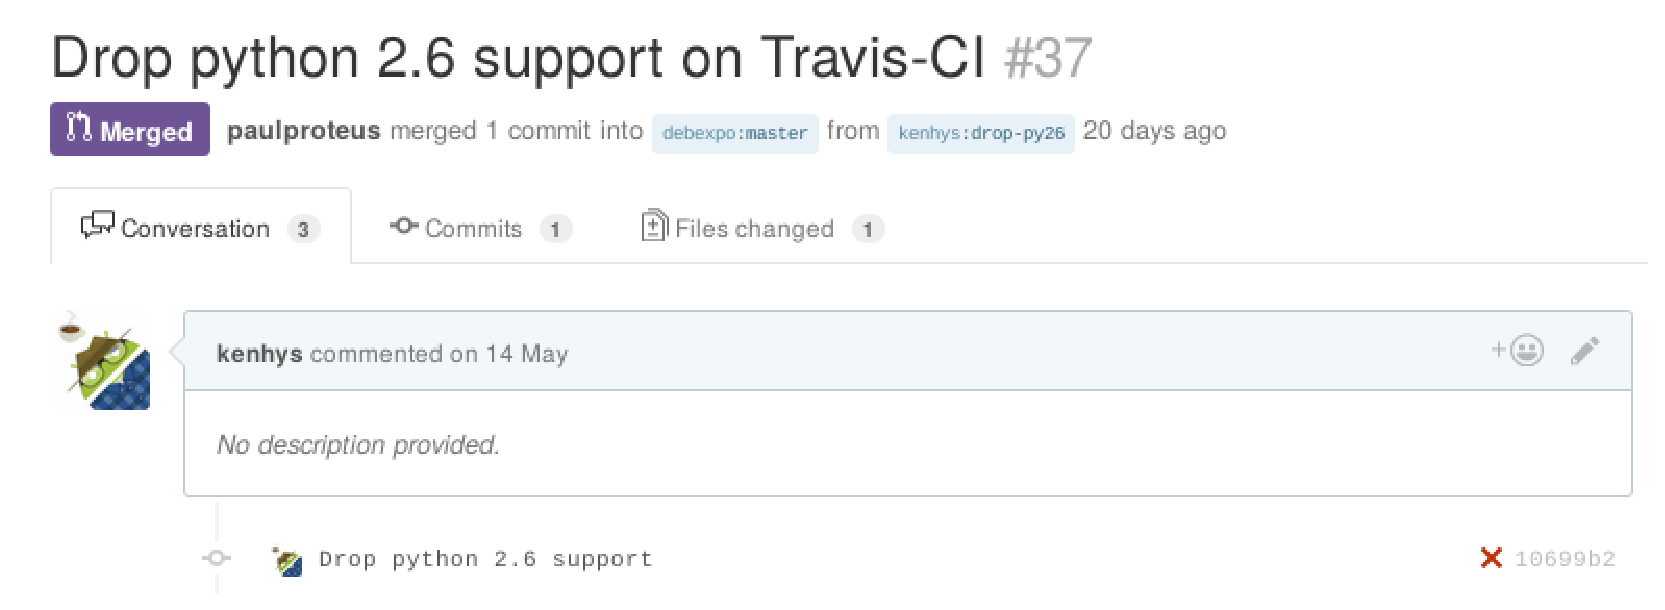
\includegraphics[width=0.7\hsize]{image201606/debexpo-pr37-drop-py26.eps}
\end{screen}

$B$3$3$^$G=$@5$7$F!"$h$&$d$/%Q%C%1!<%8$r<h$j9~$`$H$3$m$^$G$?$I$j$D$-$^$7$?!#%Q%C%1!<%8$N<h$j9~$_$O<!$N%3%^%s%I$r<B9T$7$^$9!#(B

\begin{commandline}
$ ./bin/debexpo_importer.py \
  -c /tmp/debexpo/growl-for-linux_0.8.5-1_source.changes -i development.ini --skip-gpg-check --skip-email
\end{commandline}

$B%$%s%]!<%H%9%/%j%W%H$r<B9T$7$?$i!"$"$C$5$j<h$j9~$_$G$-$:$K%H%l!<%9$rEG$-$^$7$?!#(B

\begin{commandline}
Traceback (most recent call last):
  File "./bin/debexpo_importer.py", line 60, in
  i.main()
  File "/home/vagrant/debexpo/debexpo/importer/importer.py", line 473, in main
  gpg = get_gnupg()
  File "/home/vagrant/debexpo/debexpo/lib/utils.py", line 119, in get_gnupg
  return gnupg.GnuPG(config['debexpo.gpg_path'],
  File "/home/vagrant/debexpo/venv/local/lib/python2.7/site-packages/paste/registry.py", line 146, in getitem
  return self._current_obj()[key]
  KeyError: 'debexpo.gpg_path'
\end{commandline}

gpg$B$N8!>Z$r%9%-%C%W$9$k%*%W%7%g%s$,4|BT$9$k$h$&$KF0:n$7$F$$$J$+$C$?$N$G!"%*%W%7%g%s$r@5$7$/2r<a$9$k$h$&$K(B PR\#39$B$G=$@5$7$^$7$?!#(B

\begin{screen}
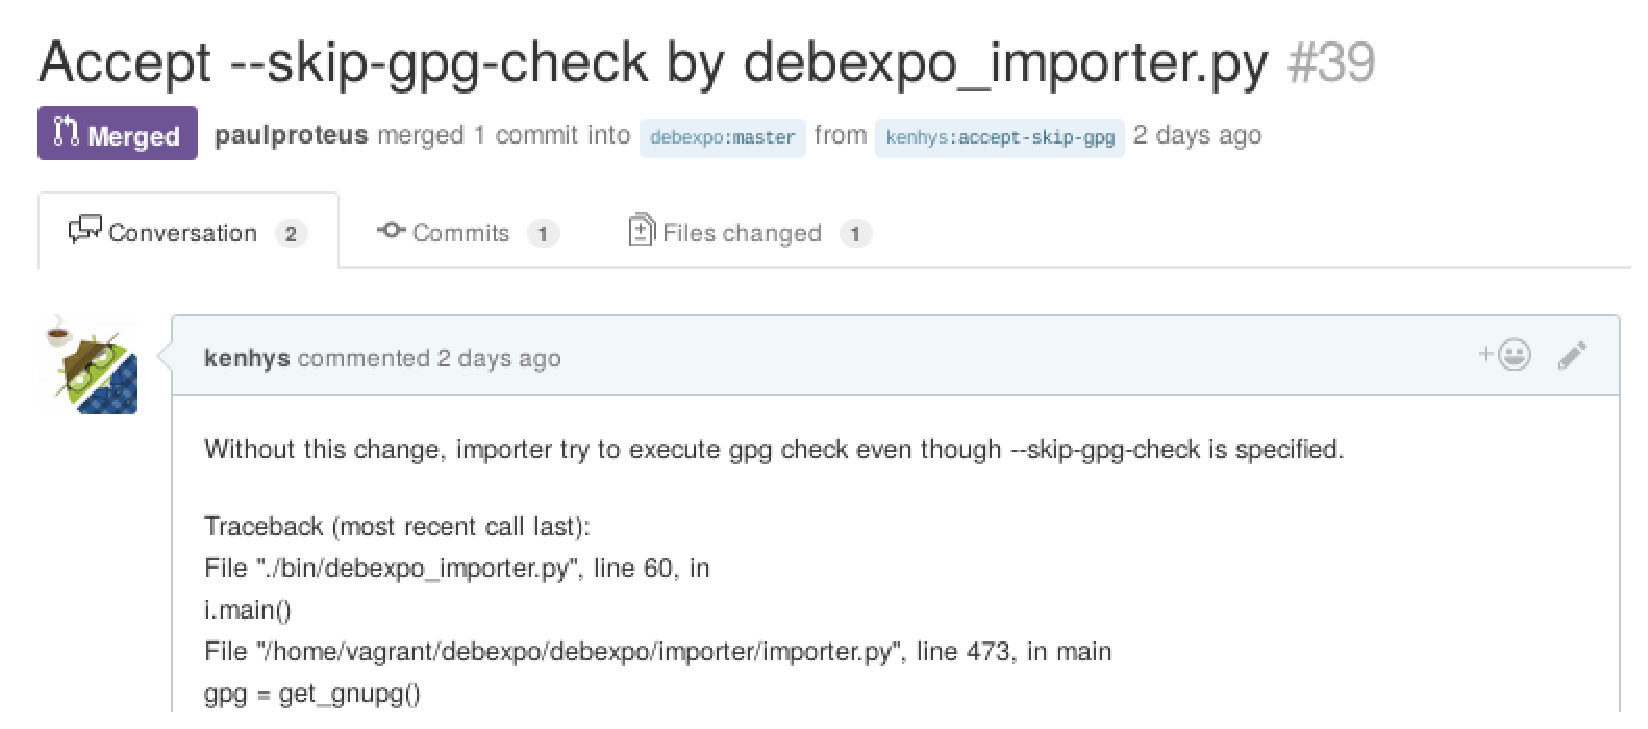
\includegraphics[width=0.7\hsize]{image201606/debexpo-pr39-skip-gpg.eps}
\end{screen}

$B$3$l$G$h$&$d$/!"<h$j9~$s$@%Q%C%1!<%8$r(BWeb$B$N2hLL$+$i3NG'$9$k$3$H$,$G$-$k$h$&$K$J$j$^$7$?!#(B

\begin{screen}
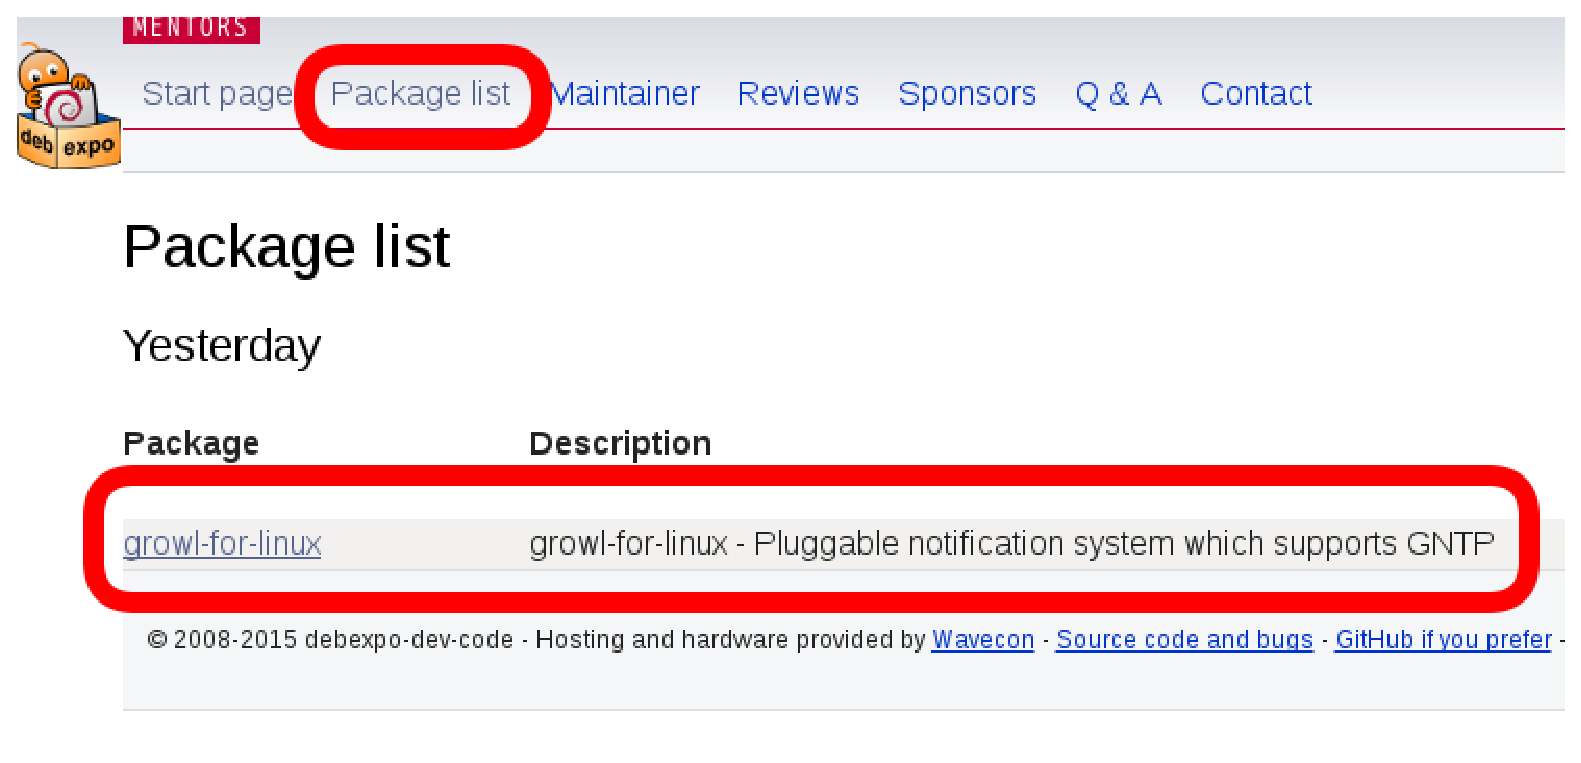
\includegraphics[width=0.7\hsize]{image201606/debexpo-package-list.eps}
\end{screen}

\subsubsection{$B$"$?$j$r$D$1$F=$@5(B}

$B%Q%C%1!<%8$r%"%C%W%m!<%I$7$F!"2hLL$+$i3NG'$G$-$k$h$&$K$J$C$?$N$G!"<!$KK\Mh$d$j$?$+$C$?(Bdebexpo$B<+BN$N2~A1$K<h$jAH$_$^$7$?!#(B
$B$^$:$O%G%#%l%/%H%j9=@.$+$i$"$?$j$r$D$1$k$3$H$K$7$^$7$?!#(B

\begin{commandline}
config
controllers
cronjobs
importer
i18n
lib
model
plugins
public
templates
tests
\end{commandline}

$B<j$,$+$j$H$J$k$N$O(BURL$B$G$9!#(B

\begin{screen}
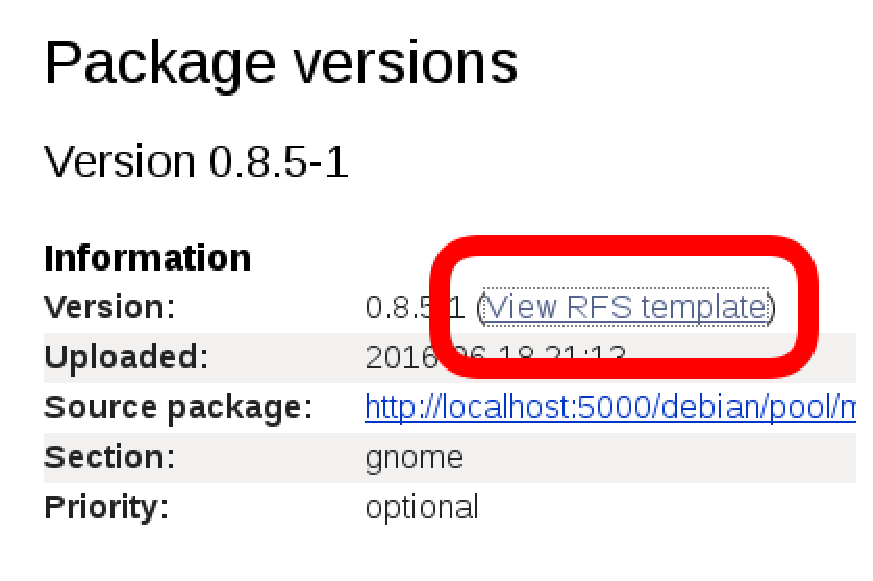
\includegraphics[width=0.7\hsize]{image201606/debexpo-investigate-rfs-template-link.eps}
\end{screen}

$BCN$j$?$$$N$O(BView RFS Template$B$N%j%s%/@h$G$9!#(B

\begin{screen}
http://localhost:5000/sponsors/rfs-howto/xxxx
\end{screen}

$B%j%s%/@h$,$o$+$C$?$N$G!"BP1~$9$k%k!<%F%#%s%0$r=hM}$9$k%3%s%H%m!<%i$N<BAu$rC5$7$F$_$?$i(Bcontrollers/sponsor.py$B$r8+$l$P$$$$$3$H$,$o$+$j$^$7$?!#(B

\begin{screen}
\begin{minted}{python}
def rfs_howto(self, packagename = None):
    c.package = None
    c.package_dir = None
    if packagename:
        package = meta.session.query(Package)
                    .filter_by(name=packagename).first()
        if package:
            c.package = package
            c.package_dir = get_package_dir(package.name)

    return render('/sponsor/rfs_howto.mako')
\end{minted}
\end{screen}

$B$3$l$KBP1~$9$k(BMako$B$N%F%s%W%l!<%H$O(Btemplates/sponsor/rfs\_howto.mako$B$K$"$k$3$H$,$o$+$j$^$7$?!#(B
$B$J$s$H$J$/8+3P$($,$"$j$^$9$M!#(B

\begin{screen}
\begin{minted}{sh}
    Package: sponsorship-requests
    Severity: normal [important for RC bugs, wishlist for new packages]

    Dear mentors,

    %if c.package:
      I am looking for a sponsor for my package "${ c.package.name }"
    %else:
      I am looking for a sponsor for my package "hello":
    %endif
\end{minted}
\end{screen}


$B$d$j$?$$$3$H$O!"(BRFS$B%F%s%W%l!<%H$+$i(B[fill in]$B$rKPLG$7!"(Bmailto:$B%j%s%/$r@8@.$7$F(BRFS$B$r=P$9$H$-$N<j4V$r7Z8:$9$k$3$H$G$9!#(B
$BEv=i$NL\O@8+$G$O!"(B\${ c.package.name }$B$H$+$"$k$N$G!"%F%s%W%l!<%H$r=q$-49$($l$P$$$$$@$1$+$H;W$C$F$$$^$7$?!#(B
$B$7$+$7!"7kO@$+$i$$$&$H$3$N0F$OL5M}$G$7$?!#$H$$$&$N$b!"I,MW$J%a%?>pJs$rJ];}$7$F$$$J$$$3$H$,L@$i$+$K$J$C$?$+$i$G$9!#;}$C$F$J$$$b$N$OI=<($G$-$^$;$s!#$=$N$?$a!"$I$&$K$+$7$F>pJs$r$+$-=8$a$J$$$H$$$1$J$$$3$H$K$J$j$^$7$?!#(B

\subsubsection{$B<}=8$9$k$K$O$I$&$9$l$P$$$$$+(B}

$B$^$:$O!"%$%s%]!<%H$N=hM}$NN.$l$rGD0.$9$kI,MW$,$"$j$^$9!#$=$7$F!"$I$N%?%$%_%s%0$G<}=8$9$Y$-$+$rCN$i$J$1$l$P$J$j$^$;$s!#$^$?ITB-$7$F$$$k>pJs$O2?$+$rCN$kI,MW$b$"$j$^$9!#(B

$B$G$O!"<B:]$N%$%s%]!<%H=hM}$O$I$N$h$&$K$J$C$F$$$k$N$G$7$g$&$+!#(B

$B%$%s%]!<%H=hM}$O!"(Bdput$B$G(Bmentors.d.n$B$X%"%C%W%m!<%I$5$l$?;~E@$G;O$^$j$^$9!#$=$7$F!"A0=hM}$,<B9T$5$l!"%Q%C%1!<%8$N%$%s%]!<%H=hM}$X$HB3$$$F$$$-$^$9!#(B
$B$b$&>/$7>\$7$/@bL@$9$k$H!"(Bdput$B$7$?%U%!%$%k$O(B/tmp/debexpo/pub$B$XJ]B8$5$l$^$9!#$=$7$F!"%$%s%]!<%HA0=hM}$G(B/tmp/debexpo$B%X0\F0$5$l$^$9!#$3$N$H$-!"(Borig.tar.gz$B$,$J$+$C$?$j$9$k$H(Breject$B%a!<%k$,Aw$i$l$^$9!#(B

$B%$%s%]!<%H$,40N;$7$?;~E@$G!"%=!<%9%Q%C%1!<%8$O(B/tmp/debexpo/files$B$X$H0\F0$5$l$F$$$^$9!#$3$N$H$-!"(B/tmp/debexpo/files$B0J2<$K$O(Bpool$B$d(Bdist,git$B%G%#%l%/%H%j$,:n@.$5$l$^$9!#(B
$B$^$?!"3F<o%Q%C%1!<%8$N>pJs$,%$%s%]!<%HCf$K%G!<%?%Y!<%9$X$HJ]B8$5$l$k$h$&$K$J$C$F$$$^$9!#(B

\subsubsection{$B<}=8$9$Y$-%G!<%?$r3NG'$9$k(B}

$B<}=8$9$k$Y$-%G!<%?$r3NDj$9$k$K$O!"%a%?>pJs$,$I$N$h$&$KJ];}$5$l$F$$$k$N$+$rGD0.$9$kI,MW$,$"$j$^$9!#$=$3$G<B:]$N%F!<%V%k$rGA$$$F$_$k$3$H$K$7$^$7$?!#(B
debexpo$B$G;HMQ$7$F$$$k<g$J%F!<%V%k$O0J2<$N(B3$B$D$G$9!#(B

\begin{itemize}
  \item packages
  \item package\_versions
  \item package\_info
\end{itemize}

packages$B%F!<%V%k$O!"%Q%C%1!<%8$N%^%9%?!<%F!<%V%k$G$9!#L>A0$d@bL@$J$I$N%a%?>pJs$rJ];}$7$F$$$^$9!#(B

\begin{screen}
\begin{minted}{sql}
sqlite> .schema packages
  CREATE TABLE packages (
      id INTEGER NOT NULL, 
      name TEXT NOT NULL, 
      user_id INTEGER, 
      description TEXT, 
      watch_counter INTEGER, 
      download_counter INTEGER, 
      needs_sponsor INTEGER NOT NULL, 
      PRIMARY KEY (id), 
      FOREIGN KEY(user_id) REFERENCES users (id)
  );
\end{minted}
\end{screen}

package\_versions$B%F!<%V%k$O%Q%C%1!<%8$NHG4IM}$N$?$a$N%F!<%V%k$G$9!#2?EY$b%"%C%W%m!<%I$9$k$H%l%3!<%I$,A}$($F$$$-$^$9!#(B

\begin{screen}
\begin{minted}{sql}
sqlite> .schema package_versions
  CREATE TABLE package_versions (
      id INTEGER NOT NULL, 
      package_id INTEGER, 
      version TEXT NOT NULL, 
      maintainer TEXT NOT NULL, 
      section TEXT NOT NULL, 
      distribution TEXT NOT NULL, 
      qa_status INTEGER NOT NULL, 
      component TEXT NOT NULL, 
      priority TEXT, 
      closes TEXT, 
      uploaded DATETIME NOT NULL, 
      PRIMARY KEY (id), 
      FOREIGN KEY(package_id) REFERENCES packages (id)
  );
\end{minted}
\end{screen}

package\_info$B%F!<%V%k$O!"%W%i%0%$%s$NE,MQ7k2L$r4IM}$7$^$9!#3F<o%a%?>pJs$rJ];}$7$F$$$^$9!#(B

\begin{screen}
\begin{minted}{sql}
sqlite> .schema package_info
CREATE TABLE package_info (
      id INTEGER NOT NULL, 
      package_version_id INTEGER, 
      from_plugin VARCHAR(200) NOT NULL, 
      outcome VARCHAR(200) NOT NULL, 
      data TEXT, 
      severity INTEGER NOT NULL, 
      PRIMARY KEY (id), 
      FOREIGN KEY(package_version_id) REFERENCES package_versions (id)
);
\end{minted}
\end{screen}

$B$?$H$($P!"(Bfrom\_plugin $B$K$O$I$N%W%i%0%$%s$+$H$$$&>pJs$rJ];}$7$F$$$^$9!#(Boutcome$B$O%(%i!<%a%C%;!<%8$J$I$N@bL@J8$rJ];}$7$F$$$^$9!#(Bdata$B$OHFMQE*$K;H$($k$h$&$K(BJSON$B%G!<%?$rJ];}$7$F$$$^$9!#(B

$B<B:]$K$I$s$J%G!<%?$,3JG<$5$l$F$$$k$+$r$_$F$_$^$7$g$&!#(Bdata$B$r$&$^$$$3$H3hMQ$9$k$H$h$5$=$&$@$H$o$+$j$^$9$M!#(B

\begin{screen}
\begin{minted}{sql}
sqlite> select * from package_info;
1|1|native|Package is not native|{"native": false}|1
2|1|maintaineremail|"Maintainer" email is the same as the uploader|{
  "user-email":   "hayashi@clear-code.com",
  "uploader-emails": [],
  "maintainer-email": "hayashi@clear-code.com",
  "user-is-maintainer": true
}|1
3|1|debianqa|Package is already in Debian|{
  "nmu": false,
  "in-debian": true,
  "is-debian-maintainer": true
}|1
\end{minted}
\end{screen}

$B$3$3$^$G$N7k2L$+$i!"%W%i%0%$%s$GDI2C$N%a%?>pJs$r<}=8$7$F!"%a!<%kMQ$N%F%s%W%l!<%HDI2C$7!">\:Y%Z!<%8$G%a%?>pJs$rI=<($7$D$D(Bmailto:$B%j%s%/@8@.$9$kJ}?K$H$7$^$7$?!#(B

\subsubsection{$B%W%i%0%$%s$N@bL@(B}

$B$3$3$^$G$N@bL@$GFC$KCG$j$J$/%W%i%0%$%s$K8@5Z$7$F$$$^$7$?!#(B
$BJdB-$7$F$*$/$H!"(Bdebexpo$B$O%W%i%0%$%s$G5!G=3HD%$9$k$h$&$K$J$C$F$$$^$9!#%Q%C%1!<%8$N%A%'%C%/$b%W%i%0%$%s$rAH$_9g$o$;$F<B8=$7$F$$$^$9!#(B

$B%W%i%0%$%s$N:n$jJ}$K$D$$$F$O!"(Bdocs/writing\_plugins.rst$B$K%5%s%W%k$N%W%i%0%$%s$N<BAuJ}K!$,>R2p$5$l$F$$$^$9!#(B
$B4JC1$K8@$&$H!"(BBasePlugin$B%/%i%9$r7Q>5$7$?(BXXXPlugin$B$H$7$F<BAu$9$l$P(BOK$B$G$9!#(B

\begin{screen}
\begin{minted}{python}
class FooPlugin(BasePlugin):

  def test_xxx(self):
    self.passed(outcome, data, severity)
    or
    self.failed(outcome, data, severity)
plugin = FooPlugin
\end{minted}
\end{screen}

$B$=$7$F!"(Bdebexpo/plugins/foo.py$B$J$I$H$7$F(Bplugins$B%G%#%l%/%H%j0J2<$KG[CV$9$k$3$H$K$J$C$F$$$^$9!#(B

$BI8=`$GMQ0U$5$l$F$$$k%W%i%0%$%s$K$O<!$N$h$&$J$b$N$,$"$j$^$9!#(B

\begin{commandline}
$ wc -l debexpo/plugins/*.py
 99 debexpo/plugins/buildsystem.py
 67 debexpo/plugins/changeslist.py
141 debexpo/plugins/closedbugs.py
 85 debexpo/plugins/controlfields.py
185 debexpo/plugins/debianqa.py
 85 debexpo/plugins/diffclean.py
 63 debexpo/plugins/distribution.py
123 debexpo/plugins/getorigtarball.py
116 debexpo/plugins/lintian.py
100 debexpo/plugins/maintaineremail.py
 69 debexpo/plugins/native.py
 77 debexpo/plugins/notuploader.py
 86 debexpo/plugins/removepackage.py
 60 debexpo/plugins/ubuntuversion.py
110 debexpo/plugins/watchfile.py
\end{commandline}

\subsubsection{$B%W%i%0%$%s$NE,MQJ}K!(B}

$B%W%i%0%$%s$r<B:]$KE,MQ$9$k$K$O!"@_Dj%U%!%$%k(B(.ini)$B$K5-=R$rDI2C$7$^$9!#(B
$B%W%i%0%$%s$G$O<!$N%?%$%_%s%0$G=hM}$r<B9T$9$k$3$H$,$G$-$^$9!#(B

\begin{itemize}
\item $B%$%s%]!<%HA0=hM}(B
\item QA$B=hM}(B
\item Debian$BF~$j$7$?;~(B
\item $B%$%s%]!<%H=hM}8e(B
\end{itemize}

$B%$%s%]!<%HA0=hM}$GE,MQ$9$k%W%i%0%$%s$O!"(Bdebexpo.plugins.post\_upload$B$K@_Dj$7$^$9!#(Bgetorigtarball$B%W%i%0%$%s$,$=$NNc$G$9!#(B
QA$B=hM}$GE,MQ$9$k%W%i%0%$%s$O!"(Bdebexpo.plugins.qa$B$K@_Dj$7$^$9!#(Blintian$B%W%i%0%$%s$,$=$NNc$G$9!#(B

$B%Q%C%1!<%8$,(BDebian$BF~$j$7$?$H$-$KE,MQ$9$k%W%i%0%$%s$O!"(Bdebexpo.plugins.post\_upload\_to\_debian$B$K@_Dj$7$^$9!#(Bremovepackage$B%W%i%0%$%s$,$=$NNc$G$9!#(B

$B%$%s%]!<%H=hM}8e$KE,MQ$9$k%W%i%0%$%s$O!"(Bdebexpo.plugins.post\_successful\_upload$B$K@_Dj$7$^$9!#(Bchangeslist$B%W%i%0%$%s$,$=$NNc$G$9!#(B

\subsubsection{$B%W%i%0%$%s$N<BAu(B}

$B$@$$$?$$$o$+$C$F$-$?$H$3$m$G!"<B:]$K%W%i%0%$%s$r<BAu$7$F$_$^$7$?!#(B
debexpo/plugins/rfstemplate.py$B$H$7$F!"<B<A(B100$B9T$J$$$/$i$$$G<BAu$G$-$^$7$?!#$d$C$F$$$k$3$H$O!"(Bdebian/changelog$B$d(Bdebian/control$B$+$iI,MW$J>pJs$rCj=P$7$F!"(Bpackage\_info$B%F!<%V%k$K%a%?>pJs$rJ];}$7!"%F%s%W%l!<%H$rI=<($9$k$H$-$K%G!<%?$r%P%$%s%I$7$FI=<($9$k$H$$$&$b$N$G$9!#(B

$B$"$H$O!"@_Dj%U%!%$%k(B(development.ini)$B$K<BAu$7$?%W%i%0%$%s$r;XDj$7$FM-8z$K$7$^$9!#(B

\begin{screen}
\begin{minted}{python}
debexpo.plugins.qa = ... rfstemplate ...
\end{minted}
\end{screen}

$B$^$?!"K:$l$:$K(Bmailto$BMQ%F%s%W%l!<%H(B(debexpo/templates/sponsor/rfs\_template.mako)$B$bDI2C$7$F$*$-$^$9!#(B

\begin{screen}
\begin{minted}{python}
  %if c.rfstemplate:
    Upstream Author : ${ c.rfstemplate['upstream-author'] }
  * URL             : ${ c.rfstemplate['upstream-url'] }
  * License         : ${ c.rfstemplate['upstream-license'] }
  %else:
    Upstream Author : [fill in name and email of upstream]
  * URL             : [fill in URL of upstreams web site]
  * License         : [fill in]
  %endif
\end{minted}
\end{screen}

$B<B:]$K(Brfstemplate$B$N%G!<%?$rI=<($5$;$kItJ,$O(Bpackage\_info$B%F!<%V%k$+$i(BJSON$B%G!<%?$r<hF@$7$F%"%5%$%s$9$k$@$1(B(debexpo/controllers/sponsor.py)$B$J$N$G!"4JC1$G$9!#(B

\begin{screen}
\begin{minted}{python}
  if latest:
    rfstemplate = meta.session.query(PackageInfo)
                    .filter_by(package_version_id=latest.id)
                    .filter_by(from_plugin='rfstemplate').first()
    if rfstemplate:
      c.rfstemplate = json.loads(rfstemplate.data)
    c.mailbody = render('/sponsor/rfs_template.mako')
  return render('/sponsor/rfs_howto.mako')
\end{minted}
\end{screen}

$B$3$3$^$G$N@.2LJ*$r(BPR\#35\footnote{\url{https://github.com/debexpo/debexpo/pull/35}}$B$H$7$F$@$7$^$7$?!#(B

\begin{screen}
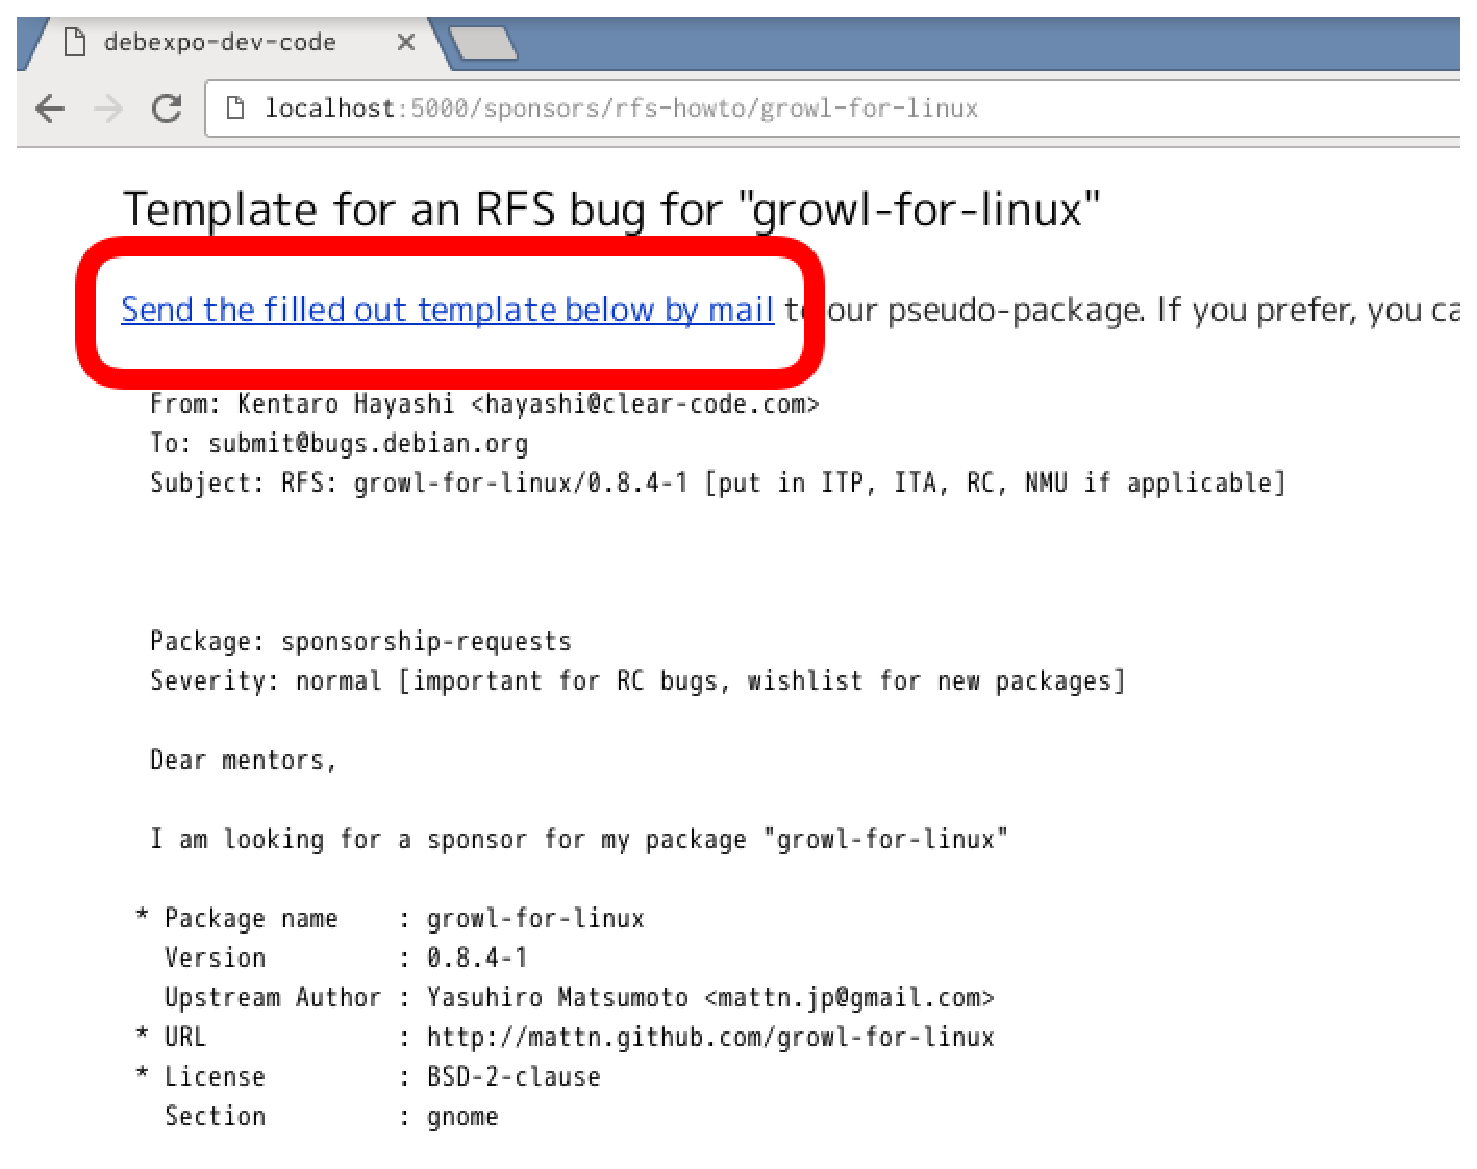
\includegraphics[width=0.7\hsize]{image201606/debexpo-pr35-take2.eps}
\end{screen}

$B%j%s%/$r%/%j%C%/$9$k$HI,MW;v9`$,Kd$a$i$l$?%F%s%W%l!<%H$r;H$C$F%a!<%i!<$,5/F0$9$k$h$&$K$J$C$F$$$^$9!#(B

\subsubsection{PR\#35$B$N7P2a(B}

$B$5$F!"(BPR$B$r$@$7$?$"$H!"$=$N8e$I$&$J$C$?$+$K$D$$$F$b>R2p$7$F$*$-$^$9!#(B

\begin{itemize}
  \item May 4 @olasd$B$5$s$+$i9%0UE*$JH?1~(B
  \item May 14 $B$I$&$J$C$?!)$H$D$D$$$F$_$k$bH?1~$J$7(B
  \item May 21 Debian$BJY6/2q$G$^$@%^!<%8$5$l$F$J$$OC$r$9$k(B
  \item $B$"$l$d$3$l$d$G$7$P$7J|CV(B
  \item June 19 @paulproteus$B$5$s$r$D$D$$$F$_$k(B
  \item June 19 20$BF|$K$_$l$k$+$b$H(B@paulproteus$B$5$s$+$iH?1~$"$j(B
\end{itemize}


\includegraphics[width=0.7\hsize]{image201606/debexpo-pr35-paulproteus.eps}

\begin{itemize}
  \item DebConf16$B$^$G$^$C$F$M!"$H$$$&$3$H$K(B
  \item DebConf16$B=*N;$9$k$b!"?JE8$J$7(B
  \item Aug 22 @paulproteus$B$5$s$K%"%5%$%s$5$l$k$bJ|CV%W%l%$$r?)$i$&(B
\end{itemize}


$B;DG0$J$,$i$$$^$@$K%l%S%e!<$7$F$b$i$($F$$$^$;$s!#(B

\subsection{$B$^$H$a(B}

$B:#2s$O(Bdebexpo$B$r%O%C%/$9$k$K;j$C$?7P0^$H!"$I$s$J%O%C%/$r$7$?$N$+$r>R2p$7$^$7$?!#(B
RFS$B%F%s%W%l!<%H$,;DG0$@$C$?$N$G$9$,!"%W%i%0%$%s$r:n@.$9$k$3$H$G(BRFS$B%F%s%W%l!<%H$r2~A1$9$k$3$H$,$G$-$^$7$?!#$?$@$7!"$^$@(BPR$B$O%^!<%8$5$l$F$$$J$$$G$9$7!"<B:]$K%G%W%m%$$5$l$k$^$G$NF;$N$j$O1s$=$&$G$9!#(B

$B:G6a$@$H!"$3$NLdBj$K4X$7$F!"(Bmentors.d.n$B$G$O$J$/%/%i%$%"%s%H%D!<%kB&$G2~A1$7$h$&$H$$$&F0$-$,$"$j$^$9!#(B

debrequest$B$H$$$&%3%^%s%I%i%$%s%D!<%k$G$$$$46$8$K(BRFS$B%F%s%W%l!<%H$r@8@.$9$k$3$H$rL\E*$K$7$F$$$k$h$&$G$9!#(B
$B<B:]$K;n$7$F$_$?$$?M$O(B\url{https://lists.debian.org/debian-mentors/2016/10/msg00206.html}$B$K3+H/<T$K$h$k%"%J%&%s%9$,Ej9F$5$l$F$$$k$N$G!"$=$A$i$r;2>H$9$k$H$h$$$G$7$g$&!#(B

%201611 tokyo
%-------------------------------------------------------------------------------
\dancersection{dh\_strip\_nondeterminism $B$K$D$$$F(B}{$B5HLn(B $BM?;V?N(B}
%-------------------------------------------------------------------------------
\subsection{$B$O$8$a$K(B}

2015 $BG/$K(B debhelper $B$N(B \verb|dh(1)| $B%7!<%1%s%9$KAH$_9~$^$l$?(B
\verb|dh_strip_nondeterminism(1)| $B$G$9$,!"$3$l$,(B
$B6qBNE*$K2?$r$d$C$F$$$k$N$+D4$Y$F$_$^$7$?!#D4$Y$?%P!<%8%g%s$O(B
dh-strip-nondeterminism $B%Q%C%1!<%8$N(B 0.028-1 $B$G$9!#(B

$B$J$*!"$3$N%3%^%s%I$NL\E*$O(B reproducible builds$B!J:F8=2DG=$J%S%k%I!K$G$9$,!">\:Y$O(B
\url{https://wiki.debian.org/ReproducibleBuilds} $B$d(B
\url{https://reproducible-builds.org/} $B$J$I$r8+$k$HNI$$$G$7$g$&!#(B

$B:F8=2DG=$J%S%k%I$r<B8=$9$k$?$a!"$3$N%3%^%s%I$O%S%k%I%D!<%k$,@8@.$7$?(B
$B%G!<%?$KKd$a9~$^$l$?;~9o$J$I$r;XDj$7$?CM$K=q$-49$($^$9!#<B:]$K8+$F$$$-$^(B
$B$7$g$&!#(B

\subsection{$B6qBNNc(B}
\subsubsection{ar}
*.a $B$N$&$A(B \verb|ar archive| $B$N$b$N(B

\begin{commandline}
$ file /usr/lib/x86_64-linux-gnu/libglib-2.0.a
/usr/lib/x86_64-linux-gnu/libglib-2.0.a: current ar archive
\end{commandline}

\verb|dh_strip_nondeterminism(1)| $B$O!"%Q%C%1!<%8$N(B debian/changelog
$B%U%!%$%k$NCf$K=q$$$F$"$k;~9o$r;H$&$h$&$K$J$C$F$$$^$9!#(B
$B$3$N(B .a $B%U%!%$%k$r4^$`%Q%C%1!<%8$N(B debian/changelog $B%U%!%$%k$N;~9o$r8+$F$_$^$9!#(B
\begin{commandline}
$ dpkg -S /usr/lib/x86_64-linux-gnu/libglib-2.0.a
libglib2.0-dev: /usr/lib/x86_64-linux-gnu/libglib-2.0.a
$ dpkg-parsechangelog -l /usr/share/doc/libglib2.0-dev/changelog.Debian.gz
Source: glib2.0
Version: 2.50.2-1
Distribution: unstable
Urgency: medium
Maintainer: Michael Biebl <biebl@debian.org>
Timestamp: 1478561825
Date: Tue, 08 Nov 2016 00:37:05 +0100
Changes:
 glib2.0 (2.50.2-1) unstable; urgency=medium
 .
   * New upstream release.
   * Track stable releases in debian/watch.
\end{commandline}
$B$3$N(B \verb|Date:|$B$G;O$^$k9T!J$b$7$/$O(B\verb|Timestamp:|$B$G;O$^$k9T!K$NCM$,;H$o$l$^$9!#(B

$B%U%!%$%k$NCf$r8+$F$_$^$9!#(B
\begin{commandline}
$ env TZ=UTC 7z l /usr/lib/x86_64-linux-gnu/libglib-2.0.a | head -n 20

7-Zip [64] 16.02 : Copyright (c) 1999-2016 Igor Pavlov : 2016-05-21
p7zip Version 16.02 (locale=ja_JP.UTF-8,Utf16=on,HugeFiles=on,64 bits,4 CPUs Intel(R) Core(TM) i5-4250U CPU @ 1.30GHz (40651),ASM,AES-NI)

Scanning the drive for archives:
1 file, 1973536 bytes (1928 KiB)

Listing archive: /usr/lib/x86_64-linux-gnu/libglib-2.0.a

--
Path = /usr/lib/x86_64-linux-gnu/libglib-2.0.a
Type = Ar
Physical Size = 1973536
SubType = a

   Date      Time    Attr         Size   Compressed  Name
------------------- ----- ------------ ------------  ------------------------
2016-11-07 23:37:05 .....        84550        84550  1.txt
2016-11-07 23:37:05 .....         4584         4584  libglib_2_0_la-gallocator.o
2016-11-07 23:37:05 .....         6352         6352  libglib_2_0_la-gcache.o
$ env TZ=UTC ar tv /usr/lib/x86_64-linux-gnu/libglib-2.0.a | head -n 4
rw-r--r-- 0/0   4584 Nov  7 23:37 2016 libglib_2_0_la-gallocator.o
rw-r--r-- 0/0   6352 Nov  7 23:37 2016 libglib_2_0_la-gcache.o
rw-r--r-- 0/0   5960 Nov  7 23:37 2016 libglib_2_0_la-gcompletion.o
rw-r--r-- 0/0  11464 Nov  7 23:37 2016 libglib_2_0_la-grel.o
\end{commandline}

$B8G$a$i$l$?3F%U%!%$%k$N(B
\begin{itemize}
 \item $B%?%$%`%9%?%s%W(B (mtime) $B$r;XDj$7$?;~9o$K=q$-49$($F$$$^$9!#(B
 \item $B=jM-<T(B (owner) $B$r(B 0 $B$K>e=q$-$7$F$$$^$9!#(B
 \item $B%0%k!<%W(B (group) $B$r(B 0 $B$K>e=q$-$7$F$$$^$9!#(B
 \item $B%Q!<%_%C%7%g%s(B (mode) $B$r(B 755 $B$+(B 644 $B$N$$$:$l$+$KB7$($F$$$^$9!#(B
\end{itemize}

\subsubsection{zip}

*.zip, *.pk3, *.epub, *.whl, *.xpi, *.htb, *.zhfst $B$N$&$A(B \verb|Zip archive data|
$B$^$?$O(B \verb|EPUB document| $B$N$b$N(B

\begin{commandline}
$ file /usr/share/go-1.7/src/archive/zip/testdata/symlink.zip
/usr/share/go-1.7/src/archive/zip/testdata/symlink.zip: Zip archive data, at least v1.0 to extract
$ file /usr/share/debian-reference/debian-reference.ja.epub
/usr/share/debian-reference/debian-reference.ja.epub: Zip archive data, at least v1.0 to extract
\end{commandline}

$BD4$Y$?%Q%C%1!<%8$N;~9o$O$=$l$>$l(B
\begin{commandline}
$ dpkg -S /usr/share/go-1.7/src/archive/zip/testdata/symlink.zip
golang-1.7-src: /usr/share/go-1.7/src/archive/zip/testdata/symlink.zip
$ dpkg-parsechangelog -l /usr/share/doc/golang-1.7-src/changelog.Debian.gz | grep ^Date:
Date: Thu, 20 Oct 2016 09:10:47 +1300
\end{commandline}

\begin{commandline}
$ dpkg -S /usr/share/debian-reference/debian-reference.ja.epub
debian-reference-ja: /usr/share/debian-reference/debian-reference.ja.epub
$ dpkg-parsechangelog -l /usr/share/doc/debian-reference-ja/changelog.gz | grep ^Date:
Date: Mon, 17 Oct 2016 22:28:00 +0900
\end{commandline}
$B$G$9!#(B

$BCf?H$r8+$F$_$^$9!#(B

\begin{commandline}
$ env TZ=UTC 7z l /usr/share/go-1.7/src/archive/zip/testdata/symlink.zip | tail -n 5
   Date      Time    Attr         Size   Compressed  Name
------------------- ----- ------------ ------------  ------------------------
2016-10-19 20:10:47 .....            9            9  symlink
------------------- ----- ------------ ------------  ------------------------
2016-10-19 20:10:47                  9            9  1 files
\end{commandline}

\begin{commandline}
$ zipinfo -v /usr/share/go-1.7/src/archive/zip/testdata/symlink.zip | tail -n 36
Central directory entry #1:
---------------------------

  symlink

  offset of local header from start of archive:   0
                                                  (0000000000000000h) bytes
  file system or operating system of origin:      Unix
  version of encoding software:                   3.0
  minimum file system compatibility required:     MS-DOS, OS/2 or NT FAT
  minimum software version required to extract:   1.0
  compression method:                             none (stored)
  file security status:                           not encrypted
  extended local header:                          no
  file last modified on (DOS date/time):          2016 Oct 19 20:10:46
  file last modified on (UT extra field modtime): 2016 Oct 20 05:10:47 local
  file last modified on (UT extra field modtime): 2016 Oct 19 20:10:47 UTC
  32-bit CRC value (hex):                         8e9efad1
  compressed size:                                9 bytes
  uncompressed size:                              9 bytes
  length of filename:                             7 characters
  length of extra field:                          24 bytes
  length of file comment:                         0 characters
  disk number on which file begins:               disk 1
  apparent file type:                             binary
  Unix file attributes (100755 octal):            -rwxr-xr-x
  MS-DOS file attributes (00 hex):                none

  The central-directory extra field contains:
  - A subfield with ID 0x5455 (universal time) and 5 data bytes.
    The local extra field has UTC/GMT modification/access times.
  - A subfield with ID 0x7875 (Unix UID/GID (any size)) and 11 data bytes:
    01 04 00 00 00 00 04 00 00 00 00.

  There is no file comment.

\end{commandline}

\begin{commandline}
$ env TZ=JST-9 7z l /usr/share/debian-reference/debian-reference.ja.epub | head -n 24 | tail -n 10
   Date      Time    Attr         Size   Compressed  Name
------------------- ----- ------------ ------------  ------------------------
2016-10-17 22:28:00 D....            0            0  META-INF
2016-10-17 22:28:00 .....          255          175  META-INF/container.xml
2016-10-17 22:28:00 D....            0            0  OEBPS
2016-10-17 22:28:00 .....        10451         3596  OEBPS/apa.html
2016-10-17 22:28:00 .....       123568        16458  OEBPS/bk01-toc.html
2016-10-17 22:28:00 .....       279742        45365  OEBPS/ch01.html
2016-10-17 22:28:00 .....       306201        49878  OEBPS/ch02.html
2016-10-17 22:28:00 .....        86922        15031  OEBPS/ch03.html
$ env TZ=JST-9 7z l /usr/share/debian-reference/debian-reference.ja.epub | tail -n 4
2016-10-17 22:28:00 .....        96004        19619  OEBPS/toc.ncx
2016-10-17 22:28:00 .....           20           20  mimetype
------------------- ----- ------------ ------------  ------------------------
2016-10-17 22:28:00            2593315       425235  23 files, 2 folders
\end{commandline}
\begin{commandline}
$ env TZ=UTC zipinfo -v /usr/share/debian-reference/debian-reference.ja.epub OEBPS/ch01.html | tail -n 12
  apparent file type:                             text
  Unix file attributes (100644 octal):            -rw-r--r--
  MS-DOS file attributes (00 hex):                none

  The central-directory extra field contains:
  - A subfield with ID 0x5455 (universal time) and 5 data bytes.
    The local extra field has UTC/GMT modification/access times.
  - A subfield with ID 0x7875 (Unix UID/GID (any size)) and 11 data bytes:
    01 04 00 00 00 00 04 00 00 00 00.

  There is no file comment.

\end{commandline}

$B8G$a$i$l$?3F%U%!%$%k$N(B
\begin{itemize}
 \item $BJB$S$rL>A0=g$KD>$7$F$$$^$9!#(B
 \item DOS $B;~9o$N%U%#!<%k%I$r;XDj$7$?;~9o$K=q$-49$($F$$$^$9!#$7$+$7!"@:(B
       $BEY$,(B2$BIC$7$+$J$$$h$&$G$9!#(B
 \item $BB0@-$r(B 755 $B$+(B 644 $B$N$$$:$l$+$KB7$($F$$$^$9!#(B
 \item central directory header$B!J$H(B local header$B!K$N(B
       \begin{itemize}
	\item ID 0x5455 (\verb|UT| universal time)$B$N%U%#!<%k%I$K;~9o$,F~$C$F$$$k$N(B
	      $B$G!";XDj$7$?;~9o$K=q$-49$($F$$$^$9!#(B
	\item ID 0x7875 (\verb|ux| Unix UID/GID)$B$N%U%#!<%k%I$K$"$k(BUID$B$H(BGID$B$r(B0
	      $B$K>e=q$-$7$F$$$^$9!#(B
       \end{itemize}
\end{itemize}

\subsubsection{jar}
*.jar, *.war, *.hpi, *.apk $B$N$&$A(B \verb|Java archive| $B$^$?$O(B \verb|Zip archive| $B$N$b$N(B

\begin{commandline}
$ file ./usr/share/java/commons-lang3.jar
./usr/share/java/commons-lang3.jar: Zip archive data, at least v1.0 to extract
\end{commandline}

\begin{commandline}
$ dpkg-parsechangelog -l ./usr/share/doc/libcommons-lang3-java/changelog.Debian.gz | grep ^Date:
Date: Thu, 20 Oct 2016 19:08:15 +0200
\end{commandline}

$BCf$r8+$F$_$^$9!#(B
\begin{commandline}
$ env TZ=UTC 7z l ./usr/share/java/commons-lang3.jar | head -n 24 | tail -n 10
   Date      Time    Attr         Size   Compressed  Name
------------------- ----- ------------ ------------  ------------------------
2016-10-20 17:08:14 D....            0            0  META-INF
2016-10-20 17:08:14 .....         1844          732  META-INF/MANIFEST.MF
2016-10-20 17:08:14 .....        11358         3949  META-INF/LICENSE.txt
2016-10-20 17:08:14 .....          301          187  META-INF/NOTICE.txt
2016-10-20 17:08:14 D....            0            0  META-INF/maven
2016-10-20 17:08:14 D....            0            0  META-INF/maven/org.apache.commons
2016-10-20 17:08:14 D....            0            0  META-INF/maven/org.apache.commons/commons-lang3
2016-10-20 17:08:14 .....           91           83  META-INF/maven/org.apache.commons/commons-lang3/pom.properties
$ env TZ=UTC 7z l ./usr/share/java/commons-lang3.jar | tail -n 4
2016-10-20 17:08:14 .....         3231         1289  org/apache/commons/lang3/tuple/Pair.class
2016-10-20 17:08:14 .....         3190         1250  org/apache/commons/lang3/tuple/Triple.class
------------------- ----- ------------ ------------  ------------------------
2016-10-20 17:08:14             986869       404745  265 files, 19 folders
\end{commandline}

\begin{commandline}
$ unzip -p ./usr/share/java/commons-lang3-3.5.jar META-INF/MANIFEST.MF
Manifest-Version: 1.0
Bundle-License: http://www.apache.org/licenses/LICENSE-2.0.txt
Bundle-SymbolicName: org.apache.commons.lang3
Archiver-Version: Plexus Archiver
Implementation-Vendor-Id: org.apache
Specification-Title: Apache Commons Lang
Bundle-DocURL: http://commons.apache.org/proper/commons-lang/
Include-Resource: META-INF/LICENSE.txt=LICENSE.txt,META-INF/NOTICE.txt
 =NOTICE.txt
Require-Capability: osgi.ee;filter:="(&(osgi.ee=JavaSE)(version=1.5))"
Export-Package: org.apache.commons.lang3;version="3.5",org.apache.comm
 ons.lang3.builder;version="3.5",org.apache.commons.lang3.concurrent;v
 ersion="3.5",org.apache.commons.lang3.event;version="3.5",org.apache.
 commons.lang3.exception;version="3.5",org.apache.commons.lang3.math;v
 ersion="3.5",org.apache.commons.lang3.mutable;version="3.5",org.apach
 e.commons.lang3.reflect;version="3.5",org.apache.commons.lang3.text;v
 ersion="3.5",org.apache.commons.lang3.text.translate;version="3.5",or
 g.apache.commons.lang3.time;version="3.5",org.apache.commons.lang3.tu
 ple;version="3.5"
Bundle-Name: Apache Commons Lang
Implementation-Title: Apache Commons Lang
Bundle-Description: Apache Commons Lang, a package of Java utility cla
 sses for the  classes that are in java.lang's hierarchy, or are consi
 dered to be so  standard as to justify existence in java.lang.
Implementation-Version: 3.5
Specification-Vendor: The Apache Software Foundation
Bundle-ManifestVersion: 2
Bundle-Vendor: The Apache Software Foundation
Tool: Bnd-2.4.1.201608301338
Implementation-Vendor: The Apache Software Foundation
Bundle-Version: 3.5.0
X-Compile-Target-JDK: 1.5
Implementation-Build: ${scmBranch}@r${buildNumber}; 2016-10-20 17:08:1
 5+0000
X-Compile-Source-JDK: 1.5
Created-By: Apache Maven Bundle Plugin
Build-Jdk: 1.8.0_102
Specification-Version: 3.5

\end{commandline}

jar $B$O(B zip $B%U%!%$%k$J$N$G!"(B*.zip $B$HF1$8JQ99$b2C$($F$$$^$9!#(B

$B$5$i$K!"(B
\begin{itemize}
 \item $B3F%U%!%$%k$NJB$S$rL>A0=g$KD>$7$F$$$^$9!#$?$@(B \verb|META-INF/| $B$H(B
       \verb|META-INF/MANIFEST.MF| $B$O@hF,$K$7$F$$$k$h$&$G$9!#(B
 \item META-INF/MANIFEST.MF $B$+$i(B
       \begin{itemize}
	\item \verb|Bnd-LastModified:| $B$G;O$^$k@8@.;~9o$,=q$+$l$?9T$r:o=|$7$F$$$^$9!#(B
	\item \verb|Built-By:| $B$G;O$^$k%S%k%I$7$?%f!<%6L>$,=q$+$l$?9T$r(B
	      $B:o=|$7$F$$$^$9!#(B
	\item $B%3%s%Q%$%i$d%S%k%I%D!<%k$N%P!<%8%g%sHV9f$O;D$7$F$$$k$h$&$G(B
	      $B$9!#%3%s%Q%$%i$N%P%0=$@5Ey$rA[Dj$7$F$$$k$N$+$b$7$l$^$;$s!#(B
       \end{itemize}
 \item *.properties $B$bJQ99$7$F$$$^$9!J8e=R!K!#(B
 \item javadoc $B$J(B *.html $B$,$"$C$?$iJQ99$9$k$i$7$$$G$9!J8e=R!K!#(B
 \item *.jar $B$,$"$C$?$i:F5"E*$KJQ99$9$k$i$7$$$G$9!#(B
 \item META-INF/*.SF $B$r4^$s$@(B jar $B%U%!%$%k$O=hM}$NBP>]30$K$7$F$$$^$9(B
       (Bug\#807669)$B!#=pL>IU$-(B jar $B%U%!%$%k$K4^$^$l$k$h$&$G$9$,!"IaDL$O(B
       $B%S%k%I;~$K<+F0=pL>$7$J$$$@$m$&$H$$$&A[Dj$J$N$G$7$g$&!#(B
\end{itemize}

\subsubsection{javadoc}
*.html $B$N$&$A(B \verb|<!-- Generated by javadoc| $B$,$"$k$b$N(B

\begin{commandline}
$ grep \<html ./usr/share/doc/libcommons-lang3-java/api/org/apache/commons/lang3/StringUtils.html
<html>
$ grep '<!-- Generated by javadoc' ./usr/share/doc/libcommons-lang3-java/api/org/apache/commons/lang3/StringUtils.html
<!-- Generated by javadoc -->
\end{commandline}

$B%U%!%$%kFb$N(B
\begin{itemize}
 \item $B@8@.;~$N4D6-$N8@8l$K4p$E$$$F=q$+$l$?(Bhtml$BMWAG$N(Blang$BB0@-(B
       (\verb|<html lang=|) $B$r:o=|$7$F$$$^$9!#(B
 \item \verb|<!-- Generated by javadoc| $B9T$+$iB>$NJ8;zNs!J@8@.;~9o$d@8@.%D!<%k$N%P!<(B
       $B%8%g%sHV9f!K$r$9$Y$F:o=|$7$F$$$^$9!#%I%-%e%a%s%H$N@8@.%D!<%k$OB?(B
       $B>/%P!<%8%g%s$,JQ$o$C$F$b@8@.7k2L$OJQ$o$i$J$$A[Dj$J$N$G$7$g$&!#(B
\end{itemize}

\subsubsection{javaproperties}
*.properties $B$N$&$A(B Java $B7O$N%S%k%I%D!<%k$G<+F0@8@.$5$l$?$h$&$K8+$($k!"(B
\verb|#Generated by Apache Maven| $B$J$I$r4^$`$b$N(B

\begin{commandline}
$ unzip -p ./usr/share/java/commons-lang3-3.5.jar META-INF/maven/org.apache.commons/commons-lang3/pom.properties
#Generated by Apache Maven
version=3.5
groupId=org.apache.commons
artifactId=commons-lang3
\end{commandline}

\verb|#| $B$G;O$^$k<+F0@8@.;~9o$,=q$+$l$?9T$r:o=|$7$F$$$^$9!#(B

\subsubsection{png}
*.png $B$N$&$A(B \verb|PNG image data| $B$N$b$N(B

\begin{commandline}
$ file /usr/share/doc/debian-handbook/html/ja-JP/images/developers-map.png
/usr/share/doc/debian-handbook/html/ja-JP/images/developers-map.png: PNG image data, 750 x 450, 8-bit/color RGB, non-interlaced
$ file /usr/share/emacs/24.5/etc/images/splash.png
/usr/share/emacs/24.5/etc/images/splash.png: PNG image data, 275 x 188, 8-bit/color RGBA, non-interlaced
\end{commandline}

\begin{commandline}
$ dpkg -S /usr/share/doc/debian-handbook/html/ja-JP/images/developers-map.png
debian-handbook: /usr/share/doc/debian-handbook/html/ja-JP/images/developers-map.png
$ dpkg-parsechangelog -l /usr/share/doc/debian-handbook/changelog.gz | grep ^Date:
Date: Thu, 22 Sep 2016 16:09:44 +0200
\end{commandline}

\begin{commandline}
$ dpkg -S /usr/share/emacs/24.5/etc/images/splash.png
emacs24-common: /usr/share/emacs/24.5/etc/images/splash.png
$ dpkg-parsechangelog -l /usr/share/doc/emacs24-common/changelog.Debian.gz | grep ^Date:
Date: Mon, 05 Sep 2016 15:05:00 -0500
\end{commandline}

$BCf$r8+$F$_$^$9!#(B
\begin{commandline}
$ hd /usr/share/doc/debian-handbook/html/ja-JP/images/developers-map.png | grep tIME
00000070  00 00 07 74 49 4d 45 07  e0 09 16 0e 09 2c 4b 76  |...tIME......,Kv|
#               ^^
#              $BD9$5(B
#                              ^^^^^^ ^^ ^^ ^^ ^^ ^^
#                               2016  09 22 14 09 44
$ strings -a /usr/share/doc/debian-handbook/html/ja-JP/images/developers-map.png | grep -A1 '[tiz]EXtdate:'
%tEXtdate:create
2016-09-22T14:09:44-00:00
%tEXtdate:modify
2016-09-22T14:09:44-00:00
$ exiftool /usr/share/doc/debian-handbook/html/ja-JP/images/developers-map.png | tail -n 5
Modify Date                     : 2016:09:22 14:09:44
Datecreate                      : 2016-09-22T14:09:44-00:00
Datemodify                      : 2016-09-22T14:09:44-00:00
Image Size                      : 750x450
Megapixels                      : 0.338
\end{commandline}

$BJQ99;~9o(B (\verb|tIME|)$B!"(B\verb|date:| $B$NCM$r;XDj$7$?;~9o$K=q$-49$($F$$$^$9!#(B

\begin{commandline}
$ strings -a /usr/share/emacs/24.5/etc/images/splash.png | grep -A1 '[tiz]EXtCreation Time'
'tEXtCreation Time
2016-09-05T20:05:00-00:00
$ exiftool /usr/share/emacs/24.5/etc/images/splash.png | tail -n 4
Description                     : GNU Emacs splash image
Creation Time                   : 2016-09-05T20:05:00-00:00
Image Size                      : 275x188
Megapixels                      : 0.052
\end{commandline}

$B:n@.;~9o(B (\verb|Creation Time|) $B$r;XDj$7$?;~9o$K=q$-49$($F$$$^$9!#(B

$B<+F0@8@.$7$J$$%"!<%H%o!<%/Ey$b$"$k$H;W$$$^$9$,!"$I$A$i$+6hJL$,IU$+$J$$$+$iA4It=q$-(B
$B49$($F$$$k$N$G$7$g$&$+!#(B

\subsubsection{gettext}
*.mo, *.gmo $B$N$&$A(B \verb|GNU message catalog| $B$N$b$N(B

\begin{commandline}
$ file /usr/share/locale/ja/LC_MESSAGES/grub.mo
/usr/share/locale/ja/LC_MESSAGES/grub.mo: GNU message catalog (little endian), revision 0.0, 233 messages
$ file /usr/share/locale/ja/LC_MESSAGES/apt.mo
/usr/share/locale/ja/LC_MESSAGES/apt.mo: GNU message catalog (little endian), revision 0.0, 367 messages
\end{commandline}

$B3F%Q%C%1!<%8$N;~9o$O(B
\begin{commandline}
$ dpkg -S /usr/share/locale/ja/LC_MESSAGES/grub.mo
grub-common: /usr/share/locale/ja/LC_MESSAGES/grub.mo
$ dpkg-parsechangelog -l /usr/share/doc/grub-common/changelog.Debian.gz | grep ^Date:
Date: Tue, 01 Nov 2016 11:10:52 +0000
\end{commandline}

\begin{commandline}
$ dpkg -S /usr/share/locale/ja/LC_MESSAGES/apt.mo
apt: /usr/share/locale/ja/LC_MESSAGES/apt.mo
$ dpkg-parsechangelog -l /usr/share/doc/apt/changelog.gz | grep ^Date:
Date: Tue, 04 Oct 2016 19:43:35 +0200
\end{commandline}
$B$G$9!#(B

$BCf$r8+$F$_$k$H(B
\begin{commandline}
$ grep -a POT-Creation-Date: /usr/share/locale/ja/LC_MESSAGES/grub.mo
POT-Creation-Date: 2016-11-01 11:10+0000
\end{commandline}

\verb|POT-Creation-Date:| $B$G;O$^$k9T$K@8@.;~9o$,F~$C$F$$$k$N$G!";XDj$7$?(B
$B;~9o$K=q$-49$($F$$$^$9!#(B

$B$?$@!";XDj$7$?;~9o$h$j?7$7$$>l9g$N$_>e=q$-$7$F$$$^$9!#(B

\begin{commandline}
$ grep -a POT-Creation-Date: /usr/share/locale/ja/LC_MESSAGES/apt.mo
POT-Creation-Date: 2016-08-30 22:20+0200
\end{commandline}

$B;XDj$7$?;~9o$h$j8E$$$N$G=q$-49$($F$$$^$;$s!#(B

\subsubsection{pearregistry}

*.reg $B$N$&$A@hF,$,(B \verb|a:| $B$N$b$N(B

\begin{commandline}
$ file ./usr/share/php/.registry/services_weather.reg
./usr/share/php/.registry/services_weather.reg: ASCII text, with very long lines
$ hd ./usr/share/php/.registry/services_weather.reg | head -n 4
00000000  61 3a 32 32 3a 7b 73 3a  37 3a 22 61 74 74 72 69  |a:22:{s:7:"attri|
00000010  62 73 22 3b 61 3a 36 3a  7b 73 3a 31 35 3a 22 70  |bs";a:6:{s:15:"p|
00000020  61 63 6b 61 67 65 72 76  65 72 73 69 6f 6e 22 3b  |ackagerversion";|
00000030  73 3a 35 3a 22 31 2e 39  2e 34 22 3b 73 3a 37 3a  |s:5:"1.9.4";s:7:|
\end{commandline}

\begin{commandline}
$ dpkg-parsechangelog -l ./usr/share/doc/php-services-weather/changelog.Debian.gz | grep -e ^Date: -e ^Timestamp:
Timestamp: 1460011442
Date: Thu, 07 Apr 2016 08:44:02 +0200
\end{commandline}

\begin{commandline}
$ hd ./usr/share/php/.registry/services_weather.reg | tail -n 8
00003580  65 22 3b 73 3a 33 3a 22  65 72 75 22 3b 73 3a 34  |e";s:3:"eru";s:4|
00003590  3a 22 72 6f 6c 65 22 3b  73 3a 34 3a 22 6c 65 61  |:"role";s:4:"lea|
000035a0  64 22 3b 7d 7d 7d 73 3a  31 30 3a 22 78 73 64 76  |d";}}}s:10:"xsdv|
000035b0  65 72 73 69 6f 6e 22 3b  73 3a 33 3a 22 32 2e 30  |ersion";s:3:"2.0|
000035c0  22 3b 73 3a 31 33 3a 22  5f 6c 61 73 74 6d 6f 64  |";s:13:"_lastmod|
000035d0  69 66 69 65 64 22 3b 69  3a 31 34 36 30 30 31 31  |ified";i:1460011|
000035e0  34 34 32 3b 7d                                    |442;}|
000035e5
\end{commandline}

\verb|_lastmodified| $B$K@8@.;~9o$,=q$+$l$F$$$k$N$G!";XDj$7$?;~9o$K=q$-49$($F$$$^$9!#(B

\subsubsection{gzip}

*.gz, *.dz $B$N$&$A(B \verb|gzip compressed data| $B$N$b$N(B


\begin{itemize}
 \item $B%U%!%$%kL>(B (FNAME) $B$N:o=|(B
 \item $B%X%C%@(BCRC (FHCRC) $B$N:o=|(B
 \item $B%X%C%@Fb$N;~9o(B (mtime) $B$,6u$G$J$/?7$7$$>l9g$O=q$-49$((B
\end{itemize}
$B$r$9$k$i$7$$$s$G$9$,!"8=J*$rC5$;$^$;$s$G$7$?!#$H$$$&$N$b!"(BDebian$B%Q%C%1!<%8(B
$BFb$K$h$/$"$k(B*.gz$B%U%!%$%k!J:#$^$G$?$/$5$s8+$F$-$?(Bchangelog$B%U%!%$%k$d(Bman$B%Z!<(B
$B%8$J$I!K(B
$B$O(B\verb|dh_compress(1)|$B$,%U%!%$%kL>$d;~9o$rJ]B8$7$J$$%*%W%7%g%s$G05=L$7(B
$B$F$$$^$9!#$7$+$b(B\verb|dh(1)|$B%7!<%1%s%9$G$O(B
\verb|dh_strip_nondeterminism(1)| $B$N8e$,(B \verb|dh_compress(1)|$B$J$N$G=q$-(B
$B49$(BP>]$K$J$C$F$$$^$;$s!#(B

\begin{commandline}
$ grep -C2 dh_strip_nondeterminism /usr/bin/dh
	dh_installwm
	dh_installxfonts
	dh_strip_nondeterminism
	dh_compress
	dh_fixperms
\end{commandline}

\subsection{$B$^$H$a(B}

\verb|dh_strip_nondeterminism(1)| $B$O!":F8=2DG=$J%S%k%I$K$7$F$$$/$KEv$?$j!"(B
$B%S%k%I7k2L!J%P%$%J%j$J$I!K$r;H$&:]$K$ODL>oITMW$J@8@.;~9o$J$I$N>pJs$r7h$^$C$?(B
$BCM$K=q$-49$($F$$$^$9!#(B

$B%S%k%I%D!<%kEy$r3+H/$7$F$$$kJ}$O!"$3$l$KMj$i$:!"$=$b$=$b%S%k%I;~$K$3$&$$$C(B
$B$?>pJs$rKd$a9~$^$J$$$h$&$K$7$?$[$&$,$h$$$G$7$g$&!#(B

$BIaDL$N%Q%C%1!<%8%a%s%F%J$NJ}$O!"$3$N%3%^%s%I$O$3$N$h$&$J=q$-49$($r$7$F$$$k$N$G(B
$B!J(Bman$B%Z!<%8$K$O(B\verb|good guesses|$B$7$F$$$k$H=q$$$F$"$j$^$9$,!K%P%0$C$F$$$k(B
$B$b$N$,$"$C$?$iJs9p$7$^$7$g$&!#(B

reproducible builds $B$K6=L#$,$"$kJ}$O!"$b$C$H=q$-49$($?$[$&$,$$$$$+$b$7$l(B
$B$J$$$b$N$,$"$C$?$i%P%0Js9p$7$?$[$&$,$h$$$+$b$7$l$^$;$s!#(B

\subsection{$B;29MJ88%(B}

dh-strip-nondeterminism 0.028-1, p7zip-full, unzip, zip, libarchive-zip-perl,
libimage-exiftool-perl $B3F%Q%C%1!<%8(B

%201609 tokyo
%-------------------------------------------------------------------------------
\dancersection{DEP5/Machine-readable debian/copyright $B:F9M(B}{$B4d>>(B $B?.MN(B}
%-------------------------------------------------------------------------------

\subsection{$B$O$8$a$K(B}

Debian $B%=!<%9%Q%C%1!<%8$K$O(B debian/copyright $B%U%!%$%k$,$"$j!"$3$N%U%!%$%k$K$O(B
$BBP>]%=%U%H%&%'%"$N%i%$%;%s%9!"%3%T!<%i%$%H$,=q$+$l$F$$$^$9!#(B
2009$BG/0JA0$OFC$K%U%)!<%^%C%H$b$J$/!"%i%$%;%s%9$bJq3gE*$J=q$-J}$G$7$?!#(B
$BNc$($P(B gcc-defaults $B%=!<%9%Q%C%1!<%8$N(B debian/copyright $B%U%!%$%k$O?^(B
\ref{fig:non-dep5-copyright}$B$N$h$&$K$J$C$F$$$^$9!#(B

\begin{figure}[htbp]
\begin{center}
\begin{commandline}
gcc-defaults is Copyright (C) 2000, 2001, 2006, 2009 Debian.

These scripts are free software; you can redistribute it and/or modify it
under the terms of the GNU General Public License as published by the
Free Software Foundation; either version 2, or (at your option) any
later version.

On Debian GNU/Linux systems, the complete text of the GNU General
Public License can be found in `/usr/share/common-licenses/GPL'.

The c89 and c99 man pages are taken from netbsd:

Copyright (c) 1999 The NetBSD Foundation, Inc.
All rights reserved.
($B>JN,(B)
\end{commandline}
\end{center}
\caption{DEP5 $BHs=`5r$J(B debian/copyright}
\label{fig:non-dep5-copyright}
\end{figure}


2010$BG/:"(B Debian$B3+H/<T$G$"$k(BSteve Langasek $B$i$K$h$C$F(B debian/copyright $B%U%!%$%k$r(B
$B5!3#=hM}$G$-$k%U%)!<%^%C%H$K@Z$jBX$(!"<+F0%A%'%C%/$J$I$,$G$-$k$h$&$K$9$k$?$a!"(B
DEP5 / Machine-readable debian/copyright $B!J0J2<!"(BDEP5$B!K$,:vDj$5$l$^$7$?(B(\url{http://dep.debian.net/deps/dep5/})$B!#(B
$B:vDj8e(B BTS 609160 $B$K$h$C$F(B Debian Policy $B$K<h$j9~$^$l!"(BDebian Policy $B$N0lIt(B(Debian Policy 12.5$B!"%*%W%7%g%J%k07$$(B)
$B$H$J$C$F$$$^$9!#:G?7%P!<%8%g%s$O(B 1.0 $B$G$"$j!":G?7HG$O(B
\url{https://www.debian.org/doc/packaging-manuals/copyright-format/1.0/}
$B$+$i;2>H$G$-$^$9!#(B

$B:vDj$+$i(B6$BG/6a$/7P$A!"B?$/$N%Q%C%1!<%8$,(BDEP5 $B=`5r$N(B debian/copyright 
$B$K$J$C$F$$$^$9!#$7$+$7$3$N%U%!%$%k!"(BDebian Policy $B$G$b%*%W%7%g%J%k07$$$H$$$&(B
$B$3$H$b$"$j!"0lEY:n$C$F$7$^$&$H$"$^$j99?7$7$J$$$H$$$&$3$H$b$"$j!"FbMF$,JQ99$5$l(B
$B$:$=$N$^$^B3$1$k$H$$$&LdBj$b$"$j$^$9!#(B
$B:#2s$O(B DEP5 $B$K$D$$$F$N%U%)!<%^%C%H$N>R2p$H!"(Bdebian/copyright $B%U%!%$%k$N99?7J}K!$K$D$$$F(B
$B>R2p$7$^$9!#(B

\subsection{DEP5 $B%U%)!<%^%C%H$K$D$$$F(B}

DEP5$B$N%U%)!<%^%C%H$O%X%C%@!<It$H%U%!%$%kIt$GJ,$1$i$l$^$9!#(B
$B%X%C%@!<It$K$O%=%U%H%&%'%"A4BN$K4X$o$k>pJs!"Nc$($PHRI[85$dO"Mm@h!"(B
$B%U%!%$%kIt$K$O%U%!%$%kKh$N%3%T!<%i%$%H$H%i%$%;%s%9$r5-=R$7$^$9!#(B

$B%X%C%@!<It$GMxMQ$G$-$k%U%#!<%k%I$O0J2<$NDL$j$G$9!#(B
\begin{itemize}

  \item Format:

        $B%U%)!<%^%C%HFbMF$,=q$+$l$?%U%!%$%k$N(BURI$B$r;XDj$7$^$9!#(B
        $B<B:]$K$O(B\url{https://www.debian.org/doc/packaging-manuals/copyright-format/1.0/}$B$r;XDj$7$^$9!#(B
        $B@N$O(Bpackaging-manuals$B$K4^$^$l$F$$$J$+$C$?$?$a!"5DO@$N>l$G$"$C$?(B wiki$B$N(BURI
        $B!J(B\url{http://wiki.debian.org/Proposals/CopyrightFormat}$B!K$d(B\texttt{http://} $B$,;XDj$5$l$F$$$k(B
        $B%Q%C%1!<%8$b$"$j$^$9!#(B

  \item Upstream-Name:

        $B%"%C%W%9%H%j!<%`$N%=%U%H%&%'%"%Q%C%1!<%8L>$r;XDj$7$^$9!#(BDebian$B$N>l9g$O<B:]$N%=%U%H%&%'%"L>$H(BDebian$B%=!<%9(B
        $B%Q%C%1!<%8L>$,0[$J$k>l9g$,$"$j$^$9!#$3$N%U%#!<%k%I$O%*%W%7%g%s07$$$G$9!#(B

  \item Upstream-Contact:

        $B%"%C%W%9%H%j!<%`$NO"Mm@h$r;XDj$7$^$9!#$3$N%U%#!<%k%I$O%*%W%7%g%s07$$$G$9!#(B

  \item Source:

        $B%=!<%9HRI[@h$r;XDj$7$^$9!#$3$N%U%#!<%k%I$O%*%W%7%g%s07$$$G$9!#(B

  \item  Disclaimer:

        $B%=%U%H%&%'%"$NLH@U;v9`$r5-:\$7$^$9!#(Bcontrib $B$d(B non-free$B$N%Q%C%1!<%8$N>l9g$KMxMQ$7$^$9!#$3$N%U%#!<%k%I$O%*%W%7%g%s07$$$G$9!#(B

  \item  Comment:

        $B%3%a%s%H$r5-:\$7$^$9!#%=%U%H%&%'%"$N%i%$%;%s%9$,J#;($J7P0^$r;}$C$F$$$k>l9g$J$I$KMxMQ$5$l$k(B
        $B$h$&$G$9!#$3$N%U%#!<%k%I$O%*%W%7%g%s07$$$G$9!#(B

  \item  License:

         $B%i%$%;%s%9$r5-:\$7$^$9!#:G=i$N9T$G$O%i%$%;%s%9$N%7%g!<%H%P!<%8%g%s$r;XDj$7!"(B
         $B<!$N9T$+$i$O%m!<%+%k%U%!%$%k%7%9%F%`$K$"$k%i%$%;%s%9%U%!%$%k$X$N%Q%9!J(B
         $BNc(B:/usr/share/common-licenses/GPL-2$B!K$H!"%=%U%H%&%'%"J]>Z$NJ|4~$dLdBj$,(B
         $B$"$C$?>l9g$NDLCNJ}K!$J$I$r4^$a$?J8>O$r5-:\$7$^$9!#(B
         $B$b$7%i%$%;%s%9%U%!%$%k$,%m!<%+%k%U%!%$%k%7%9%F%`$K$J$$>l9g$OA4J85-:\$9(B
         $B$kI,MW$,$"$j$^$9!#(B
         $B%7%g!<%H%P!<%8%g%s$N%i%$%;%s%9$N5-:\J}K!$G$9$,!"(BGNU GPL version2 or later $B$N>l9g$O(B\texttt{GPL-2+}$B!"(B
         Creative Commons Attribution Share Alike license 3.0$B$N>l9g$O(B\texttt{CC-BY-SA-3.0}$B$H;XDj$9$k(B
         $B$3$H$,$G$-$^$9!#(B
         $B>\:Y$O(B\url{https://www.debian.org/doc/packaging-manuals/copyright-format/1.0/#license-short-name}$B$r;2>H$7$F$/$@$5$$!#(B
         $B$3$N%U%#!<%k%I$O%*%W%7%g%s07$$$G$9!#(B

  \item  Copyright:

         $B%3%T!<%i%$%H%[%k%@!<$r5-:\$7$^$9!#$3$N%U%#!<%k%I$O%*%W%7%g%s07$$$G$9!#(B

\end{itemize}

$B>e5-$N%U%)!<%^%C%H$@$1$G$O!"%U%!%$%kKh$K%i%$%;%s%9$,0[$J$k>l9g!"5-:\$9$k$3$H$,Fq(B
$B$7$/$J$j$^$9!#$J$N$G!"K\%U%)!<%^%C%H$G$O!">e5-$K2C$(!"%U%!%$%kKh$N%i%$%;%s%9$H%3(B
$B%T!<%i%$%H%[%k%@!<$r5-:\$9$k%U%!%$%kIt$N%U%)!<%^%C%H$,$"$j$^$9!#(B
$B%U%!%$%kIt$GMxMQ$G$-$k%U%#!<%k%I$O0J2<$NDL$j$G$9!#(B
\begin{itemize}
  \item  Files:

         $B%U%!%$%k$r5-:\$7$^$9!#F1$8%i%$%;%s%9!"%3%T!<%i%$%H%[%k%@!<$r$b$D%U%!%$(B
         $B%k$r$^$H$a$F5-:\$9$k$3$H$,$G$-$^$9!#(B
  \item  Copyright:

         $B%3%T!<%i%$%H%[%k%@!<$r5-:\$7$^$9!#(B
  \item  License:

         $B%i%$%;%s%9$r5-:\$7$^$9!#5-:\J}K!$O>e5-$NJ}K!$HF1$8$G$9!#%i%$%;%s%9$OF1(B
         $B$8$@$,!"%U%!%$%kKh$K%3%T!<%i%$%H%[%k%@!<$,0[$J$k>l9g!"%i%$%s%;%s%9$N%7(B
         $B%g!<%H%P!<%8%g%s$N$_$r5-:\$7!"K\J8$r$^$H$a$F5-:\$9$k$3$H$b$G$-$^$9!#(B
         $BNc$r?^(B\ref{fig:repeat-license}$B$K<($7$^$9!#(B

\begin{figure}[htbp]
\begin{center}
\begin{commandline}
Files: *
Copyright: foo bar <foo@example.org>
License: GPL-2+

Files: debian/*
Copyright: Nobuhiro Iwamatsu <iwamatsu@debian.org>
License: GPL-2+
 This program is free software; you can redistribute it
 and/or modify it under the terms of the GNU General Public
 License as published by the Free Software Foundation; either
 version 2 of the License, or (at your option) any later
 version.
 .
 This program is distributed in the hope that it will be
 useful, but WITHOUT ANY WARRANTY; without even the implied
 warranty of MERCHANTABILITY or FITNESS FOR A PARTICULAR
 PURPOSE.  See the GNU General Public License for more
 details.
 .
 You should have received a copy of the GNU General Public
 License along with this package; if not, write to the Free
 Software Foundation, Inc., 51 Franklin St, Fifth Floor,
 Boston, MA  02110-1301 USA
 .
 On Debian systems, the full text of the GNU General Public
 License version 2 can be found in the file
 `/usr/share/common-licenses/GPL-2'.
\end{commandline}
\end{center}
\caption{$B%i%$%;%s%9$N7+$jJV$7Nc(B}
\label{fig:repeat-license}
\end{figure}


  \item  Comment:

         $B%3%a%s%H$r5-:\$7$^$9!#$3$N%U%#!<%k%I$O%*%W%7%g%s07$$$G$9!#(B
\end{itemize}

$B>e5-$rAH$_9g$o$;$k$3$H$K$h$C$F(B debian/copyright $B%U%!%$%k$r(B DEP5 $B=`5r$K(B
$B$7$^$9!#(B

$B$=$NB>!"5<;w%U%#!<%k%I$H$7$F(B $B%i%$%;%s%9$N5vBz>pJs$r5-:\$9$k(B License-Grant $B%U%#!<%k%I!"(B
$B%i%$%s%;%9%U%!%$%k$X$N%Q%9$r5-:\$9$k(B License-Reference $B%U%#!<%k%I$r;H$C$F$$$k(B
$B>l9g$b$"$j$^$9!J(B\debianbug{786450}$B!K!#(B

\subsection{DEP5 $B$NLdBjE@$HBP:v(B}

$B>e5-$G@bL@$7$?%U%)!<%^%C%H$rDj5A$7$?(B DEP5 $B$G$9$,!"%U%!%$%k$,B?$/$J$k$[$I5-:\$9$k(B
$B$3$H$,Fq$7$/$J$j!"$"$^$j99?7$5$l$J$$$H$$$&LdBj$,$"$j$^$9!#$^$?(B DEP5 $B$O%]%j%7!<$G(B
$B$b%*%W%7%g%J%k$J$N$G!"0\9T$,$"$^$j?J$s$G$$$J$$$H$$$&LdBj$b$"$j$^$9!#(B

$B$3$3$G$O(B debian/copyright $B$N(B DEP5 $B2=$H99?7J}K!$K$D$$$F>R2p$7$^$9!#(B

\subsubsection{licensecheck $B$r;H$C$?(BDEP5 $B%U%)!<%^%C%H2=(B}

$B;XDj$7$?%G%#%l%/%H%j$K$"$k%U%!%$%k$N%i%$%;%s%9$H%3%T!<%i%$%H%[%k%@!<$r=PNO$9$k(B
licensecheck $B$H$$$&%D!<%k$,$"$j$^$9(B($B?^(B\ref{fig:licensecheck})$B!#(B
$B$3$l$O@N$O(B devscripts $B$GDs6!$5$l$F$$$^$7$?$,!"J,N%$5$l(B(\debianbug{828872})$B!"(Blicensecheck $B%Q%C%1!<%8$G(B
$BDs6!$5$l$k$h$&$K$J$j$^$7$?!#(B
\texttt{-r} $B%*%W%7%g%s$G;XDj$7$?%G%#%l%/%H%j$r:F5"E*$K8!:w!"(B\texttt{--copyright} $B%*%W%7%g(B
$B%s$G%3%T!<%i%$%H%[%k%@!<$r=PNO$9$k$h$&$K$7$^$9!#(B
$B<B9TNc$r?^(B\ref{fig:licensecheck}$B$K<($7$^$9!#(B

\begin{figure}[htbp]
\begin{center}
\begin{commandline}
$ licensecheck -r --copyright .
ell/io.h: LGPL (v2.1 or later)
  [Copyright: 2011-2014 Intel Corporation. All rights reserved]

ell/dbus.c: LGPL (v2.1 or later)
  [Copyright: 2011-2014 Intel Corporation. All rights reserved]
($B>JN,(B)
\end{commandline}
\end{center}
\caption{licensecheck$B%3%^%s%I<B9TNc(B}
\label{fig:licensecheck}
\end{figure}

$B$3$l$@$1$G$O(B DEP5 $B%U%)!<%^%C%H$K$J$i$J$$$?$a!"(Bcdbs$B$GDs6!$5$l$F$$$k(B
/usr/lib/cdbs/licensecheck2dep5 $B$r;H$C$F@07A$7$^$9!J?^(B
\ref{fig:update-copyright-by-cdbs}$B!K!#(B

\begin{figure}[htbp]
\begin{center}
\begin{commandline}
$ licensecheck -r --copyright .  | /usr/lib/cdbs/licensecheck2dep5

Format: http://www.debian.org/doc/packaging-manuals/copyright-format/1.0/
Upstream-Name: FIXME
Upstream-Contact: FIXME
Source: FIXME
Disclaimer: Autogenerated by CDBS

Files: ./ell/base64.c
 ./ell/base64.h
 ./ell/checksum.c
 $B!JCfN,!K(B 
 ./unit/test-uuid.c
Copyright: 2011-2014, Intel Corporation.
  2011-2015, Intel Corporation.
  2011-2016, Intel Corporation.
  2015, Intel Corporation.
  2016, Intel Corporation.
License: LGPL (v2.1 or later)
 FIXME
$B!J>JN,!K(B 
\end{commandline}
\end{center}
\caption{licensecheck2dep5 $B$K$h$k(B debian/copyright $B99?7J}K!(B}
\label{fig:update-copyright-by-cdbs}
\end{figure}

DEP5$B%U%)!<%^%C%H$K$7$F=PNO$7$F$/$l$^$9$,!"(BLicense $B%U%#!<%k%I$,(B\texttt{FIXME}
$B$K$J$C$F$$$?$j!"(BASCII $B0J30$NJ8;z$OJ8;z2=$1$9$k$J$I!"40`z$J=PNO$O$7$F$/$l$J$$$?$a!"(B
$B@8@.$5$l$?%F%-%9%H$r=$@5$9$kI,MW$,$"$j$^$9!#(B

\subsubsection{cme $B$r;H$C$?(B DEP5 $B%U%)!<%^%C%H2=$H(B debian/copyright $B$N99?7(B}

licensecheck2dep5 $B$h$j>/$78-$$=PNO$r$7$F$/$l$k%D!<%k$H$7$F(B cme $B$,$"$j$^$9!#(B
$B$3$l$OHFMQE*$J@_Dj%U%!%$%kJT=8%D!<%k$J$N$G$9$,!"(Blibconfig-model-dpkg-perl $B%Q%C%1(B
$B!<%8(B $B$r%$%s%9%H!<%k$9$k$3$H$K$h$j!"(Bdebian $B%Q%C%1!<%8MQ$N%b%G%k$,;H$($k$h$&$K$J$j$^$9!#(B
debian/copyright $B$r99?7$7$?$$>l9g$K$O(B \texttt{dpkg-copyright} $B%*%W%7%g%s$r;H$$$^$9!#(B
$B<B9T$9$k$H(BDEP5 $B%U%)!<%^%C%H$G(B debian/copyright $B$K=PNO$7$^$9!J?^(B\ref{fig:update-copyright}$B!K!#(B
\footnote{cme $B$O(B "cme check dpkg-control" $B$H$$$C$?(B debian/control $B$KBP$9$k%A%'%C%/$J$I$b(B
$B9T$($^$9!#$3$NOC$O$^$?:#EY!#(B}

\begin{figure}[htbp]
\begin{center}
\begin{commandline}
$ sudo apt-get install cme libconfig-model-dpkg-perl
$ cme update dpkg-copyright
cme: using Dpkg::Copyright model
updating data
$B!J>JN,!K(B
\end{commandline}
\end{center}
\caption{CME $B$K$h$k(B debian/copyright $B99?7J}K!(B}
\label{fig:update-copyright}
\end{figure}

$B$^$?(Blibconfig-model-tkui-perl $B%Q%C%1!<%8$r%$%s%9%H!<%k$9$k$H(BGUI$B$GJT=8$G$-$k$h$&$J$j(B
$B$^$9(B($B?^(B\ref{fig:edit-copyright}$B!"?^(B\ref{fig:cme-gui})$B!#(B

\begin{figure}[htbp]
 \begin{minipage}{0.5\hsize}
\begin{center}
\begin{commandline}
$ sudo apt-get install libconfig-model-tkui-perl
debian/copyright $B$rJT=8$7$?$$>l9g(B
$ cme edit dpkg-copyright
debian/copyright $B$r99?7$7$?8e!"JT=8$7$?$$>l9g(B
$ cme update dpkg-copyright --edit
$B%(%G%#%?$GD>@\JT=8$G$bBg>fIW$G$9!#(B
$ cme update dpkg-copyright
$ vi debian/copyright
\end{commandline}
\end{center}
\caption{debian/copyright $BJT=8J}K!(B}
\label{fig:edit-copyright}
 \end{minipage}
 \begin{minipage}{0.5\hsize}
\begin{center}
\includegraphics[width=0.7\hsize]{image201609/cme-gui.png}
\end{center}
\caption{cme GUI$B5/F02hLL(B}
\label{fig:cme-gui}
 \end{minipage}
\end{figure}

$B$3$l$b(Blicensecheck2dep5$B$HF1MM!"40`z$J=PNO$O$7$F$/$l$J$$$?$a!"=PNO(B
$B$5$l$?(B debian/copyright $B%U%!%$%k$r3NG'$7$F=$@5$9$kI,MW$,$"$j$^$9!#(B
$B$^$?(BUTF-8$B$KBP1~$7$F$$$k$?$a!"(BASCII$BJ8;z0J30$G$b@5$7$/=hM}$7$F$/$l$^$9!#(B

\subsubsection{debmake $B$r;H$C$?(B debian/copyright $B$N(B DEP5$B%U%)!<%^%C%H2=(B}

debmake $B%3%^%s%I$N(B \texttt{-cc} $B%*%W%7%g%s$r;H$C$F(BDEP5$B%U%)!<%^%C%H2=$5$l$?(B
debian/copyright $B$r:n@.$9$k$3$H$b$G$-$^$9!#(B

\begin{commandline}
$ debmake -cc > debian/copyright
\end{commandline}

cme $B$H$N0c$$$O(B $B%U%!%$%k$rNs5s$9$kE@!J(Bcme$B$O%o%$%k%I%+!<%I(B($\ast$)$B$G$^$H$a$k(B)
$B$H(B $BITMW$J%U%!%$%k!JNc(B debian/copyright$B!K$NFbMF$^$G3NG'$7$F$7$^$&$J$I$,$"$j$^$9!#(B
debmake $B$O(B $B%=!<%9%Q%C%1!<%8:n@.%5%]!<%H%D!<%k$J$N$G!"99?75!G=$,$^$@$J$$$N$@$H(B
$B;W$$$^$9!#8D?ME*$K$O:#$N$H$3$m(B debian $B%G%#%l%/%H%j0J2<$N%U%!%$%k%A%'%C%/$K$b(B
$B;H$($k(B cme $B$r$*A&$a$7$^$9!#(B

\subsubsection{license-reconcile $B$K$h$k(B debian/copyright $B%A%'%C%/%5%]!<%H(B}


license-reconcile $B$r;H$&$3$H$K$h$C$F!"(B
cme $B$J$I$GJaB*$G$-$J$$%U%!%$%k$N%i%$%;%s%9$d%3%T!<%i%$%H$,(B debian/copyright $B$,=q$+$l$F$$$k$+!"%A%'%C%/(B
$B$G$-$k$h$&$K$9$k%D!<%k$H$7$F(B\texttt{license-reconcile} $B$,$"$j$^$9!#(B
$B$3$l$O(B\texttt{license-reconcile}$B%Q%C%1!<%8$K$h$C$FDs6!$5$l$F$$$^$9!#(B
$BNc$($P!":#$^$GA4$F$N%U%!%$%k$,(B\texttt{GPL-3+}$B$G%i%$%;%s%9$5$l$F$$$?%W%m%0%i%`(B
$B!J?^(B\ref{fig:example-copyright}$B!K$K(B
\texttt{GPL-2+}$B$G%i%$%;%s%9$5$l$F$$$k(B\texttt{hoge.png} $B%U%!%$%k$,<h$j9~$^$l$?(B
$B$H$7$^$9!#%P%$%J%j%U%!%$%k$J$N$G(B cme $B$J$I$G$O8!CN$G$-$^$;$s!#(B

\begin{figure}[htbp]
\begin{center}
\begin{commandline}
Files: *
Copyright: 2016 foo bar <foo@example.org>
License: GPL-3+
\end{commandline}
\end{center}
\caption{debian/copyright $BNc(B}
\label{fig:example-copyright}
\end{figure}

debian/copyright $B$K5-:\$5$l$F$$$k$+%A%'%C%/$G$-$k$h$&$K$9$k$?$a!"(B
\texttt{debian/license-reconcile.yml} $B%U%!%$%k$rMQ0U$7!"?^(B
\ref{fig:example-license-reconcile}$B$N$h$&$JFbMF$r5-=R$7$^$9!#(B

\begin{figure}[htbp]
\begin{center}
\begin{commandline}
Rules:
 rules:
  -
   Glob: hoge.png
   License: GPL-2+
   Copyright: 2016 foo bar <foo@example.org>
\end{commandline}
\end{center}
\caption{debian/license-reconcile.yml $BNc(B}
\label{fig:example-license-reconcile}
\end{figure}

\texttt{license-reconcile}$B%3%^%s%I(B $B$r<B9T$9$k$H0J2<$N$h$&$J%3%T!<%i%$%H%_%9%^%C%A%(%i!<(B
$B$,=PNO$5$l$^$9!J?^(B\ref{fig:example-license-reconcile}$B!K!#(B

\begin{figure}[htbp]
\begin{center}
\begin{commandline}
$ license-reconcile
License mismatch: File hoge.png has license GPL-2+ which does not match GPL-3+.\
at /usr/share/perl5/Debian/LicenseReconcile/App.pm line 222, <GEN0> line 3.
\end{commandline}
\end{center}
\caption{license-reconcile $B<B9TNc(B}
\label{fig:example-license-reconcile}
\end{figure}

debian/copyright $B$K(B \texttt{hoge.png} $B$K4X$9$k%U%#!<%k%I!J?^(B
\ref{fig:example-update-copyright}$B!K$rDI2C$7!":FEY(B
\texttt{license-reconcile} $B%3%^%s%I$r<B9T$9$k$H%i%$%s%;%s%9%U%#!<%k%I%A%'%C%/%(%i!<$,(B
$B=PNO$5$l$J$/$J$j$^$9!#(B

\begin{figure}[htbp]
\begin{center}
\begin{commandline}
Files: hoge.png
Copyright: foo bar <foo@example.org>
License: GPL-2+
 This program is free software: you can redistribute it and/or modify
 it under the terms of the GNU General Public License as published by
 the Free Software Foundation, either version 2 of the License, or
 (at your option) any later version.
$B!J>JN,!K(B
\end{commandline}
\end{center}
\caption{debian/copyright $BDI5-Nc(B}
\label{fig:example-update-copyright}
\end{figure}

\subsubsection{debian $B%Q%C%1!<%8B&$NBP1~(B}

$B>e5-$G$O(B licensecheck $B$d(B cme $B$H$$$C$?(B $B%D!<%k$r;H$&$3$H$K$h$C$F(B debian/copyright $B%U%!%$%k$r(B
DEP5 $B%U%)!<%^%C%H$K@Z$jBX$($k$3$H$,$G$-$k$3$H$r@bL@$7$^$7$?$,!"(Bdebian/rules $B$K%A(B
$B%'%C%/MQ$N%?!<%2%C%H$rDI2C$9$k$3$H$N$h$C$F!"%Q%C%1!<%8$N%a%s%F%J%s%9@-$,8~>e$7$^(B
$B$9!#?^(B\ref{fig:example-update-rules} $B$N$h$&$K(B debian/rules $B$XDI5-$7(B
\texttt{debian/rules update-debian-copyright}$B$r<B9T$9$k$3$H$K$h$j!"(BDEP 5 $B%U%)!<(B
$B%^%C%H(B $B$N(B debian/copyright $B$r(B debian/copyright.auto $B$K=PNO$7$^$9!#(B

\begin{figure}[htbp]
\begin{center}
\begin{commandline}
# cme $B$r;H$&>l9g(B
update-debian-copyright:
	cme update dpkg-copyright -file debian/copyright.auto
# licensecheck + licensecheck2dep5 $B$r;H$&>l9g(B
update-debian-copyright:
        licensecheck --copyright -r `find * -type f` | \
                /usr/lib/cdbs/licensecheck2dep5 > debian/copyright.auto
\end{commandline}
\end{center}
\caption{debian/rules $BDI5-Nc(B}
\label{fig:example-update-rules}
\end{figure}

\subsection{$B$^$H$a(B}

DEP5 $B%U%)!<%^%C%H$N4JC1$JFbMF>R2p$H!"(Bdebian/copyright $B$N(B DEP5 $B%U%)!<%^%C%H$9$k$?(B
$B$a$N%D!<%k$N;H$$J}!"(Bdebian $B%Q%C%1!<%8$G$NMxMQJ}K!$K$D$$$F@bL@$7$^$7$?!#(B
$B0J2<!"$^$H$a$G$9!#(B
\begin{itemize}
\item DEP 5 $B$O(B Debian $B%]%j%7!<$N0lIt!#$7$+$7%*%W%7%g%J%k07$$!#(B
$B%U%)!<%^%C%H>\:Y$O(B
\url{https://www.debian.org/doc/packaging-manuals/copyright-format/1.0/}$B$^$?$O(B
\url{/usr/share/doc/debian-policy/copyright-format-1.0.txt.gz}$B$K$"$k!#(B

\item licensecheck $B%D!<%k$K$h$C$F(B $B%=!<%9$+$i$N%i%$%;%s%9$H%3%T!<%i%$%H%[%k%@!<$r(B
$BCj=P2DG=!#$=$N$^$^$G$O(BDEP5$B%U%)!<%^%C%H$K$J$i$J$$$?$a!"(Blicensecheck2dep5$B$r;H$&!#(B
\item cme $B$H(B libconfig-model-dpkg-perl $B$r;H$&$3$H$K$h$C$F(B licensecheck +
licensecheck2dep5 $BF1MM$N$3$H$,2DG=!#4d>>$N$*4+$a$O$3$A$i!#(B
\item license-reconcile $B$r;H$&$3$H$K$h$C$F(B cme $B$J$I$GJd40$G$-$J$$%U%!%$%k$N%A%'(B
$B%C%/$,$G$-$k!#(B
\item $BKh2s(B cme $B$d(B licencecheck $B$J$I$N%3%^%s%I$r<B9T$9$k$N$G$O$J$/!"(Bdebian/rules 
$B$K=q$$$F$*$/$H%a%s%F%J%s%9$,3Z$K$J$k!#(B
\end{itemize}

%201607 tokyo
%-------------------------------------------------------------------------------
\dancersection{Debian Installer Screen$BBP1~(B $BG[I[;qNA;2>H(B}{Roger}
%-------------------------------------------------------------------------------

%-------------------------------------------------------------------------------
\dancersection{Debian Trivia Quiz}{}
%-------------------------------------------------------------------------------

$B$H$3$m$G!"$_$J$5$s(B Debian $B4XO"$NOCBj$K$*$$$D$$$F$$$^$9$+!)(BDebian$B4XO"$NOC(B
$BBj$O%a!<%j%s%0%j%9%H$r$h$s$G$$$k$HDI@W$G$-$^$9!#$?$@$h$s$G$$$k$@$1$G$O$O(B
$B$j$"$$$,$J$$$N$G!"M}2rEY$N%F%9%H$r$7$^$9!#FC$K0l?M$@$1$G$O0UL#$,$o$+$i$J(B
$B$$$H$3$m$b$"$k$+$bCN$l$^$;$s!#$_$s$J$G0l=o$KFI$s$G$_$^$7$g$&!#(B

$B:#2s$N=PBjHO0O$O(B\url{debian-devel-announce@lists.debian.org} $B$d(B \url{debian-devel@lists.debian.org}$B$KEj9F$5$l$?(B
$BFbMF$H(BDebian Project News$B$+$i$G$9!#(B

\small
\begin{multicols}{2}
%; whizzy-master ../debianmeetingresume201311.tex
% $B0J>e$N@_Dj$r$7$F$$$k$?$a!"$3$N%U%!%$%k$G(B M-x whizzytex $B$9$k$H!"(Bwhizzytex$B$,MxMQ$G$-$^$9!#(B
%

\santaku
{stable$BHG$N(Bjessie$B$G$bDs6!$,3+;O$5$l$?(Biceweasel$B$N%"%C%W%G!<%H!#%Q%C%1!<%8L>$,JQ$o$C$F$$$^$9!#2?$K$J$C$?$G$7$g$&$+(B}
{iceweasel-esr}
{firefox}
{firefox-esr}
{firefox-esr}
{$B%j!<%,%kLdBj$,$R$HCJMn$7!"(Bdebian$B$G$b(Bfirefox$B$H$7$FDs6!$G$-$k$3$H$K$J$j$^$7$?!#=>Mh$N(Bjessie$B$G$O(Biceweasel ver38esr$B$,Ds6!$5$l$F$$$^$7$?!#:#2s$O(Bfirefox-esr$B%Q%C%1!<%8$H$7$F(Bver45esr$B$NDs6!$,3+;O$5$l$^$7$?!#(B}

\santaku
{Debian Administrator$B!G(Bs Hanbook(Debian$B4IM}<T%O%s%I%V%C%/(B)$B$H$$$&%I%-%e%a%s%H$,$"$j$^$9!#KDBg$JNL$N%I%-%e%a%s%H$G$"$j$^$9$,!"$D$$$KF|K\8lHG$,%j%j!<%9$5$l$^$7$?!#K]Lu:n6H$KB?Bg$J9W8%$r$7$F$$$?$@$$$?J}$OC/$G$7$g$&$+!#(B}
{Ryuunosuke Ayanokouzi}
{Norimitsu Sugimoto}
{Hideki Yamane}
{Ryuunosuke Ayanokouzi}
{Debian$B4IM}<T%O%s%I%V%C%/$OL5NA$N(Bweb$BHG5Z$SEE;R=q@RHG!"M-NA$N=q@RHG$,$"$j$^$9!#:#8e$NK]Lu:n6H7QB3$N$?$a$K4sIU$rJg$C$F$$$^$9!#$J$*!"%j%j!<%9%"%J%&%s%9$N%Z!<%8$O<!$N(BURL$B$O<!$NDL$j$G$9!#(B\url{https://debian-handbook.info/2016/get-the-japanese-version-of-the-debian-administrators-handbook/}}

%; whizzy-master ../debianmeetingresume201311.tex
% $B0J>e$N@_Dj$r$7$F$$$k$?$a!"$3$N%U%!%$%k$G(B M-x whizzytex $B$9$k$H!"(Bwhizzytex$B$,MxMQ$G$-$^$9!#(B
%

\santaku
{$B$D$$@hF|=*N;$7$?(Bdebconf16$B!#3+:E>l=j$O$I$3$@$C$?$G$7$g$&$+!#(B}
{Montreal, Canada}
{Cape Town, South Africa}
{Kyoto, Japan}
{B}
{\url{https://debconf16.debconf.org/}$B$N0FFb$K$"$k$H$*$j!"Fn%"%U%j%+$N%1!<%W%?%&%s$G9T$o$l$^$7$?!#F|K\$+$i;22C$7$??M$,$$$^$9$N$G!"8e$G$I$s$J46$8$@$C$?$+J9$$$F$_$^$7$g$&!#NcG/DL$j$G$"$l$P!"%;%C%7%g%s$N%S%G%*$,8eF|8x3+$5$l$k$H;W$$$^$9!#(B}

\santaku
{Debconf16$B$G$O<!$N%j%j!<%9!V(BStretch$B!W$N%9%1%8%e!<%k$r9pCN$7$^$7$?!#0lHV:G=i$K9T$o$l$k(BTransition freeze$B$NM=Dj$O$$$D$G$7$g$&$+(B}
{2016-11-05}
{2016-12-05}
{2017-02-05}
{A}
{Transition freeze$B$,(B2016-11-05$B!"(BMandatory 10-day migrations$B$,(B2016-12-05$B!"(BSoft freeze$B$,(B2017-01-05$B!"(BFull freeze$B$,(B2017-02-05$B$NM=Dj$H$J$C$F$$$^$9!#?7$7$$%Q%C%1!<%8$r(BStretch$B$K4^$a$?$$>l9g$O$*Aa$a$K!#(B}

%; whizzy-master ../debianmeetingresume201311.tex
% $B0J>e$N@_Dj$r$7$F$$$k$?$a!"$3$N%U%!%$%k$G(B M-x whizzytex $B$9$k$H!"(Bwhizzytex$B$,MxMQ$G$-$^$9!#(B
%

\santaku
{question}
{a}
{b}
{c}
{B}
{desc}

%; whizzy-master ../debianmeetingresume201311.tex
% $B0J>e$N@_Dj$r$7$F$$$k$?$a!"$3$N%U%!%$%k$G(B M-x whizzytex $B$9$k$H!"(Bwhizzytex$B$,MxMQ$G$-$^$9!#(B
%

\santaku
{quiz1}
{a}
{b}
{c}
{B}
{desc}

%; whizzy-master ../debianmeetingresume201311.tex
% 以上の設定をしているため、このファイルで M-x whizzytex すると、whizzytexが利用できます。
%

\santaku
{HPエンタープライズ社からDebian Projectへサーバを寄付していだきました。このサーバを使ってdebian.orgのサービスの載せ替えが実施されます。さて、どの組み合わせが正しいでしょうか}
{ftp-master.debian.orgとwww.debian.org}
{ftp-master.debian.orgとsecurity.debian.org}
{www.debian.orgとsecurity.debian.org}
{B}
{寄付いただいたサーバはカナダ、アメリカ、オーストラリアにあるサーバの更新に利用する予定です。具体的にはDebianの主要サービスであるftp-master.debian.orgとsecurity.debian.orgに割り当てし、その他のコアサービスの向上にも役立てる予定です。\url{https://www.debian.org/News/2016/20161003}}

\end{multicols}
\normalsize

%for less page
%\printindex

\newpage

\begin{center}
$BK\;qNA$N%i%$%;%s%9$K$D$$$F(B
\end{center}

$BK\;qNA$O%U%j!<!&%=%U%H%&%'%"$G$9!#$"$J$?$O!"(BFree Software
Foundation $B$,8xI=$7$?(BGNU GENERAL PUBLIC LICENSE$B$N!V%P!<%8%g%s#2!W$b$7$/$O$=$l0J9_(B
$B$,Dj$a$k>r9`$K=>$C$FK\%W%m%0%i%`$r:FHRI[$^$?$OJQ99$9$k$3$H$,$G$-(B
$B$^$9!#(B

$BK\%W%m%0%i%`$OM-MQ$H$O;W$$$^$9$,!"HRI[$K$"$?$C$F$O!";T>l@-5Z$SFC(B
$BDjL\E*E,9g@-$K$D$$$F$N0EL[$NJ]>Z$r4^$a$F!"$$$+$J$kJ]>Z$b9T$J$$$^(B
$B$;$s!#>\:Y$K$D$$$F$O(BGNU GENERAL PUBLIC LICENSE $B$r$*FI$_$/$@$5$$!#(B

\begin{multicols}{2}
 \begin{fontsize}{6}{6}
 \begin{verbatim}
		    GNU GENERAL PUBLIC LICENSE
		       Version 2, June 1991

 Copyright (C) 1989, 1991 Free Software Foundation, Inc.
	51 Franklin St, Fifth Floor, Boston, MA  02110-1301  USA
 Everyone is permitted to copy and distribute verbatim copies
 of this license document, but changing it is not allowed.

			    Preamble

  The licenses for most software are designed to take away your
freedom to share and change it.  By contrast, the GNU General Public
License is intended to guarantee your freedom to share and change free
software--to make sure the software is free for all its users.  This
General Public License applies to most of the Free Software
Foundation's software and to any other program whose authors commit to
using it.  (Some other Free Software Foundation software is covered by
the GNU Library General Public License instead.)  You can apply it to
your programs, too.

  When we speak of free software, we are referring to freedom, not
price.  Our General Public Licenses are designed to make sure that you
have the freedom to distribute copies of free software (and charge for
this service if you wish), that you receive source code or can get it
if you want it, that you can change the software or use pieces of it
in new free programs; and that you know you can do these things.

  To protect your rights, we need to make restrictions that forbid
anyone to deny you these rights or to ask you to surrender the rights.
These restrictions translate to certain responsibilities for you if you
distribute copies of the software, or if you modify it.

  For example, if you distribute copies of such a program, whether
gratis or for a fee, you must give the recipients all the rights that
you have.  You must make sure that they, too, receive or can get the
source code.  And you must show them these terms so they know their
rights.

  We protect your rights with two steps: (1) copyright the software, and
(2) offer you this license which gives you legal permission to copy,
distribute and/or modify the software.

  Also, for each author's protection and ours, we want to make certain
that everyone understands that there is no warranty for this free
software.  If the software is modified by someone else and passed on, we
want its recipients to know that what they have is not the original, so
that any problems introduced by others will not reflect on the original
authors' reputations.

  Finally, any free program is threatened constantly by software
patents.  We wish to avoid the danger that redistributors of a free
program will individually obtain patent licenses, in effect making the
program proprietary.  To prevent this, we have made it clear that any
patent must be licensed for everyone's free use or not licensed at all.

  The precise terms and conditions for copying, distribution and
modification follow.

		    GNU GENERAL PUBLIC LICENSE
   TERMS AND CONDITIONS FOR COPYING, DISTRIBUTION AND MODIFICATION

  0. This License applies to any program or other work which contains
a notice placed by the copyright holder saying it may be distributed
under the terms of this General Public License.  The "Program", below,
refers to any such program or work, and a "work based on the Program"
means either the Program or any derivative work under copyright law:
that is to say, a work containing the Program or a portion of it,
either verbatim or with modifications and/or translated into another
language.  (Hereinafter, translation is included without limitation in
the term "modification".)  Each licensee is addressed as "you".

Activities other than copying, distribution and modification are not
covered by this License; they are outside its scope.  The act of
running the Program is not restricted, and the output from the Program
is covered only if its contents constitute a work based on the
Program (independent of having been made by running the Program).
Whether that is true depends on what the Program does.

  1. You may copy and distribute verbatim copies of the Program's
source code as you receive it, in any medium, provided that you
conspicuously and appropriately publish on each copy an appropriate
copyright notice and disclaimer of warranty; keep intact all the
notices that refer to this License and to the absence of any warranty;
and give any other recipients of the Program a copy of this License
along with the Program.

You may charge a fee for the physical act of transferring a copy, and
you may at your option offer warranty protection in exchange for a fee.

  2. You may modify your copy or copies of the Program or any portion
of it, thus forming a work based on the Program, and copy and
distribute such modifications or work under the terms of Section 1
above, provided that you also meet all of these conditions:

    a) You must cause the modified files to carry prominent notices
    stating that you changed the files and the date of any change.

    b) You must cause any work that you distribute or publish, that in
    whole or in part contains or is derived from the Program or any
    part thereof, to be licensed as a whole at no charge to all third
    parties under the terms of this License.

    c) If the modified program normally reads commands interactively
    when run, you must cause it, when started running for such
    interactive use in the most ordinary way, to print or display an
    announcement including an appropriate copyright notice and a
    notice that there is no warranty (or else, saying that you provide
    a warranty) and that users may redistribute the program under
    these conditions, and telling the user how to view a copy of this
    License.  (Exception: if the Program itself is interactive but
    does not normally print such an announcement, your work based on
    the Program is not required to print an announcement.)

These requirements apply to the modified work as a whole.  If
identifiable sections of that work are not derived from the Program,
and can be reasonably considered independent and separate works in
themselves, then this License, and its terms, do not apply to those
sections when you distribute them as separate works.  But when you
distribute the same sections as part of a whole which is a work based
on the Program, the distribution of the whole must be on the terms of
this License, whose permissions for other licensees extend to the
entire whole, and thus to each and every part regardless of who wrote it.

Thus, it is not the intent of this section to claim rights or contest
your rights to work written entirely by you; rather, the intent is to
exercise the right to control the distribution of derivative or
collective works based on the Program.

In addition, mere aggregation of another work not based on the Program
with the Program (or with a work based on the Program) on a volume of
a storage or distribution medium does not bring the other work under
the scope of this License.

  3. You may copy and distribute the Program (or a work based on it,
under Section 2) in object code or executable form under the terms of
Sections 1 and 2 above provided that you also do one of the following:

    a) Accompany it with the complete corresponding machine-readable
    source code, which must be distributed under the terms of Sections
    1 and 2 above on a medium customarily used for software interchange; or,

    b) Accompany it with a written offer, valid for at least three
    years, to give any third party, for a charge no more than your
    cost of physically performing source distribution, a complete
    machine-readable copy of the corresponding source code, to be
    distributed under the terms of Sections 1 and 2 above on a medium
    customarily used for software interchange; or,

    c) Accompany it with the information you received as to the offer
    to distribute corresponding source code.  (This alternative is
    allowed only for noncommercial distribution and only if you
    received the program in object code or executable form with such
    an offer, in accord with Subsection b above.)

The source code for a work means the preferred form of the work for
making modifications to it.  For an executable work, complete source
code means all the source code for all modules it contains, plus any
associated interface definition files, plus the scripts used to
control compilation and installation of the executable.  However, as a
special exception, the source code distributed need not include
anything that is normally distributed (in either source or binary
form) with the major components (compiler, kernel, and so on) of the
operating system on which the executable runs, unless that component
itself accompanies the executable.

If distribution of executable or object code is made by offering
access to copy from a designated place, then offering equivalent
access to copy the source code from the same place counts as
distribution of the source code, even though third parties are not
compelled to copy the source along with the object code.

  4. You may not copy, modify, sublicense, or distribute the Program
except as expressly provided under this License.  Any attempt
otherwise to copy, modify, sublicense or distribute the Program is
void, and will automatically terminate your rights under this License.
However, parties who have received copies, or rights, from you under
this License will not have their licenses terminated so long as such
parties remain in full compliance.

  5. You are not required to accept this License, since you have not
signed it.  However, nothing else grants you permission to modify or
distribute the Program or its derivative works.  These actions are
prohibited by law if you do not accept this License.  Therefore, by
modifying or distributing the Program (or any work based on the
Program), you indicate your acceptance of this License to do so, and
all its terms and conditions for copying, distributing or modifying
the Program or works based on it.

  6. Each time you redistribute the Program (or any work based on the
Program), the recipient automatically receives a license from the
original licensor to copy, distribute or modify the Program subject to
these terms and conditions.  You may not impose any further
restrictions on the recipients' exercise of the rights granted herein.
You are not responsible for enforcing compliance by third parties to
this License.

  7. If, as a consequence of a court judgment or allegation of patent
infringement or for any other reason (not limited to patent issues),
conditions are imposed on you (whether by court order, agreement or
otherwise) that contradict the conditions of this License, they do not
excuse you from the conditions of this License.  If you cannot
distribute so as to satisfy simultaneously your obligations under this
License and any other pertinent obligations, then as a consequence you
may not distribute the Program at all.  For example, if a patent
license would not permit royalty-free redistribution of the Program by
all those who receive copies directly or indirectly through you, then
the only way you could satisfy both it and this License would be to
refrain entirely from distribution of the Program.

If any portion of this section is held invalid or unenforceable under
any particular circumstance, the balance of the section is intended to
apply and the section as a whole is intended to apply in other
circumstances.

It is not the purpose of this section to induce you to infringe any
patents or other property right claims or to contest validity of any
such claims; this section has the sole purpose of protecting the
integrity of the free software distribution system, which is
implemented by public license practices.  Many people have made
generous contributions to the wide range of software distributed
through that system in reliance on consistent application of that
system; it is up to the author/donor to decide if he or she is willing
to distribute software through any other system and a licensee cannot
impose that choice.

This section is intended to make thoroughly clear what is believed to
be a consequence of the rest of this License.

  8. If the distribution and/or use of the Program is restricted in
certain countries either by patents or by copyrighted interfaces, the
original copyright holder who places the Program under this License
may add an explicit geographical distribution limitation excluding
those countries, so that distribution is permitted only in or among
countries not thus excluded.  In such case, this License incorporates
the limitation as if written in the body of this License.

  9. The Free Software Foundation may publish revised and/or new versions
of the General Public License from time to time.  Such new versions will
be similar in spirit to the present version, but may differ in detail to
address new problems or concerns.

Each version is given a distinguishing version number.  If the Program
specifies a version number of this License which applies to it and "any
later version", you have the option of following the terms and conditions
either of that version or of any later version published by the Free
Software Foundation.  If the Program does not specify a version number of
this License, you may choose any version ever published by the Free Software
Foundation.

  10. If you wish to incorporate parts of the Program into other free
programs whose distribution conditions are different, write to the author
to ask for permission.  For software which is copyrighted by the Free
Software Foundation, write to the Free Software Foundation; we sometimes
make exceptions for this.  Our decision will be guided by the two goals
of preserving the free status of all derivatives of our free software and
of promoting the sharing and reuse of software generally.

			    NO WARRANTY

  11. BECAUSE THE PROGRAM IS LICENSED FREE OF CHARGE, THERE IS NO WARRANTY
FOR THE PROGRAM, TO THE EXTENT PERMITTED BY APPLICABLE LAW.  EXCEPT WHEN
OTHERWISE STATED IN WRITING THE COPYRIGHT HOLDERS AND/OR OTHER PARTIES
PROVIDE THE PROGRAM "AS IS" WITHOUT WARRANTY OF ANY KIND, EITHER EXPRESSED
OR IMPLIED, INCLUDING, BUT NOT LIMITED TO, THE IMPLIED WARRANTIES OF
MERCHANTABILITY AND FITNESS FOR A PARTICULAR PURPOSE.  THE ENTIRE RISK AS
TO THE QUALITY AND PERFORMANCE OF THE PROGRAM IS WITH YOU.  SHOULD THE
PROGRAM PROVE DEFECTIVE, YOU ASSUME THE COST OF ALL NECESSARY SERVICING,
REPAIR OR CORRECTION.

  12. IN NO EVENT UNLESS REQUIRED BY APPLICABLE LAW OR AGREED TO IN WRITING
WILL ANY COPYRIGHT HOLDER, OR ANY OTHER PARTY WHO MAY MODIFY AND/OR
REDISTRIBUTE THE PROGRAM AS PERMITTED ABOVE, BE LIABLE TO YOU FOR DAMAGES,
INCLUDING ANY GENERAL, SPECIAL, INCIDENTAL OR CONSEQUENTIAL DAMAGES ARISING
OUT OF THE USE OR INABILITY TO USE THE PROGRAM (INCLUDING BUT NOT LIMITED
TO LOSS OF DATA OR DATA BEING RENDERED INACCURATE OR LOSSES SUSTAINED BY
YOU OR THIRD PARTIES OR A FAILURE OF THE PROGRAM TO OPERATE WITH ANY OTHER
PROGRAMS), EVEN IF SUCH HOLDER OR OTHER PARTY HAS BEEN ADVISED OF THE
POSSIBILITY OF SUCH DAMAGES.

		     END OF TERMS AND CONDITIONS

	    How to Apply These Terms to Your New Programs

  If you develop a new program, and you want it to be of the greatest
possible use to the public, the best way to achieve this is to make it
free software which everyone can redistribute and change under these terms.

  To do so, attach the following notices to the program.  It is safest
to attach them to the start of each source file to most effectively
convey the exclusion of warranty; and each file should have at least
the "copyright" line and a pointer to where the full notice is found.

    <one line to give the program's name and a brief idea of what it does.>
    Copyright (C) <year>  <name of author>

    This program is free software; you can redistribute it and/or modify
    it under the terms of the GNU General Public License as published by
    the Free Software Foundation; either version 2 of the License, or
    (at your option) any later version.

    This program is distributed in the hope that it will be useful,
    but WITHOUT ANY WARRANTY; without even the implied warranty of
    MERCHANTABILITY or FITNESS FOR A PARTICULAR PURPOSE.  See the
    GNU General Public License for more details.

    You should have received a copy of the GNU General Public License
    along with this program; if not, write to the Free Software
    Foundation, Inc., 51 Franklin St, Fifth Floor, Boston, MA  02110-1301 USA


Also add information on how to contact you by electronic and paper mail.

If the program is interactive, make it output a short notice like this
when it starts in an interactive mode:

    Gnomovision version 69, Copyright (C) year  name of author
    Gnomovision comes with ABSOLUTELY NO WARRANTY; for details type `show w'.
    This is free software, and you are welcome to redistribute it
    under certain conditions; type `show c' for details.

The hypothetical commands `show w' and `show c' should show the appropriate
parts of the General Public License.  Of course, the commands you use may
be called something other than `show w' and `show c'; they could even be
mouse-clicks or menu items--whatever suits your program.

You should also get your employer (if you work as a programmer) or your
school, if any, to sign a "copyright disclaimer" for the program, if
necessary.  Here is a sample; alter the names:

  Yoyodyne, Inc., hereby disclaims all copyright interest in the program
  `Gnomovision' (which makes passes at compilers) written by James Hacker.

  <signature of Ty Coon>, 1 April 1989
  Ty Coon, President of Vice

This General Public License does not permit incorporating your program into
proprietary programs.  If your program is a subroutine library, you may
consider it more useful to permit linking proprietary applications with the
library.  If this is what you want to do, use the GNU Library General
Public License instead of this License.
 \end{verbatim}
 \end{fontsize}
\end{multicols}

\begin{center}
$B%=!<%9%3!<%I$K$D$$$F(B
\end{center}

$B%=!<%9%3!<%I$O(B Git $B$r;H$C$F(B\url{git://anonscm.debian.org/tokyodebian/monthly-report.git}
$B$+$i%@%&%s%m!<%I$G$-$^$9!#0J2<$KJ}K!$r<($7$^$9!#(B

\begin{commandline}
$ git clone git://anonscm.debian.org/tokyodebian/monthly-report.git
\end{commandline}
%$

\begin{center}
$BK\;qNA$N%i%$%;%s%9$K$D$$$F(B
\end{center}

$BK\;qNA$O%U%j!<!&%=%U%H%&%'%"$G$9!#$"$J$?$O!"(BFree Software
Foundation $B$,8xI=$7$?(BGNU GENERAL PUBLIC LICENSE$B$N(B "$B%P!<%8%g%s#2(B"$B$b$7$/$O$=$l0J9_(B
$B$,Dj$a$k>r9`$K=>$C$FK\%W%m%0%i%`$r:FHRI[$^$?$OJQ99$9$k$3$H$,$G$-(B
$B$^$9!#(B

$BK\%W%m%0%i%`$OM-MQ$H$O;W$$$^$9$,!"HRI[$K$"$?$C$F$O!";T>l@-5Z$SFC(B
$BDjL\E*E,9g@-$K$D$$$F$N0EL[$NJ]>Z$r4^$a$F!"$$$+$J$kJ]>Z$b9T$J$$$^(B
$B$;$s!#>\:Y$K$D$$$F$O(BGNU GENERAL PUBLIC LICENSE $B$r$*FI$_$/$@$5$$!#(B

\begin{multicols}{2}
 \begin{fontsize}{6}{6}
 \begin{verbatim}
            GNU GENERAL PUBLIC LICENSE
               Version 2, June 1991

 Copyright (C) 1989, 1991 Free Software Foundation, Inc.
    51 Franklin St, Fifth Floor, Boston, MA  02110-1301  USA
 Everyone is permitted to copy and distribute verbatim copies
 of this license document, but changing it is not allowed.

                Preamble

  The licenses for most software are designed to take away your
freedom to share and change it.  By contrast, the GNU General Public
License is intended to guarantee your freedom to share and change free
software--to make sure the software is free for all its users.  This
General Public License applies to most of the Free Software
Foundation's software and to any other program whose authors commit to
using it.  (Some other Free Software Foundation software is covered by
the GNU Library General Public License instead.)  You can apply it to
your programs, too.

  When we speak of free software, we are referring to freedom, not
price.  Our General Public Licenses are designed to make sure that you
have the freedom to distribute copies of free software (and charge for
this service if you wish), that you receive source code or can get it
if you want it, that you can change the software or use pieces of it
in new free programs; and that you know you can do these things.

  To protect your rights, we need to make restrictions that forbid
anyone to deny you these rights or to ask you to surrender the rights.
These restrictions translate to certain responsibilities for you if you
distribute copies of the software, or if you modify it.

  For example, if you distribute copies of such a program, whether
gratis or for a fee, you must give the recipients all the rights that
you have.  You must make sure that they, too, receive or can get the
source code.  And you must show them these terms so they know their
rights.

  We protect your rights with two steps: (1) copyright the software, and
(2) offer you this license which gives you legal permission to copy,
distribute and/or modify the software.

  Also, for each author's protection and ours, we want to make certain
that everyone understands that there is no warranty for this free
software.  If the software is modified by someone else and passed on, we
want its recipients to know that what they have is not the original, so
that any problems introduced by others will not reflect on the original
authors' reputations.

  Finally, any free program is threatened constantly by software
patents.  We wish to avoid the danger that redistributors of a free
program will individually obtain patent licenses, in effect making the
program proprietary.  To prevent this, we have made it clear that any
patent must be licensed for everyone's free use or not licensed at all.

  The precise terms and conditions for copying, distribution and
modification follow.

            GNU GENERAL PUBLIC LICENSE
   TERMS AND CONDITIONS FOR COPYING, DISTRIBUTION AND MODIFICATION

  0. This License applies to any program or other work which contains
a notice placed by the copyright holder saying it may be distributed
under the terms of this General Public License.  The "Program", below,
refers to any such program or work, and a "work based on the Program"
means either the Program or any derivative work under copyright law:
that is to say, a work containing the Program or a portion of it,
either verbatim or with modifications and/or translated into another
language.  (Hereinafter, translation is included without limitation in
the term "modification".)  Each licensee is addressed as "you".

Activities other than copying, distribution and modification are not
covered by this License; they are outside its scope.  The act of
running the Program is not restricted, and the output from the Program
is covered only if its contents constitute a work based on the
Program (independent of having been made by running the Program).
Whether that is true depends on what the Program does.

  1. You may copy and distribute verbatim copies of the Program's
source code as you receive it, in any medium, provided that you
conspicuously and appropriately publish on each copy an appropriate
copyright notice and disclaimer of warranty; keep intact all the
notices that refer to this License and to the absence of any warranty;
and give any other recipients of the Program a copy of this License
along with the Program.

You may charge a fee for the physical act of transferring a copy, and
you may at your option offer warranty protection in exchange for a fee.

  2. You may modify your copy or copies of the Program or any portion
of it, thus forming a work based on the Program, and copy and
distribute such modifications or work under the terms of Section 1
above, provided that you also meet all of these conditions:

    a) You must cause the modified files to carry prominent notices
    stating that you changed the files and the date of any change.

    b) You must cause any work that you distribute or publish, that in
    whole or in part contains or is derived from the Program or any
    part thereof, to be licensed as a whole at no charge to all third
    parties under the terms of this License.

    c) If the modified program normally reads commands interactively
    when run, you must cause it, when started running for such
    interactive use in the most ordinary way, to print or display an
    announcement including an appropriate copyright notice and a
    notice that there is no warranty (or else, saying that you provide
    a warranty) and that users may redistribute the program under
    these conditions, and telling the user how to view a copy of this
    License.  (Exception: if the Program itself is interactive but
    does not normally print such an announcement, your work based on
    the Program is not required to print an announcement.)

These requirements apply to the modified work as a whole.  If
identifiable sections of that work are not derived from the Program,
and can be reasonably considered independent and separate works in
themselves, then this License, and its terms, do not apply to those
sections when you distribute them as separate works.  But when you
distribute the same sections as part of a whole which is a work based
on the Program, the distribution of the whole must be on the terms of
this License, whose permissions for other licensees extend to the
entire whole, and thus to each and every part regardless of who wrote it.

Thus, it is not the intent of this section to claim rights or contest
your rights to work written entirely by you; rather, the intent is to
exercise the right to control the distribution of derivative or
collective works based on the Program.

In addition, mere aggregation of another work not based on the Program
with the Program (or with a work based on the Program) on a volume of
a storage or distribution medium does not bring the other work under
the scope of this License.

  3. You may copy and distribute the Program (or a work based on it,
under Section 2) in object code or executable form under the terms of
Sections 1 and 2 above provided that you also do one of the following:

    a) Accompany it with the complete corresponding machine-readable
    source code, which must be distributed under the terms of Sections
    1 and 2 above on a medium customarily used for software interchange; or,

    b) Accompany it with a written offer, valid for at least three
    years, to give any third party, for a charge no more than your
    cost of physically performing source distribution, a complete
    machine-readable copy of the corresponding source code, to be
    distributed under the terms of Sections 1 and 2 above on a medium
    customarily used for software interchange; or,

    c) Accompany it with the information you received as to the offer
    to distribute corresponding source code.  (This alternative is
    allowed only for noncommercial distribution and only if you
    received the program in object code or executable form with such
    an offer, in accord with Subsection b above.)

The source code for a work means the preferred form of the work for
making modifications to it.  For an executable work, complete source
code means all the source code for all modules it contains, plus any
associated interface definition files, plus the scripts used to
control compilation and installation of the executable.  However, as a
special exception, the source code distributed need not include
anything that is normally distributed (in either source or binary
form) with the major components (compiler, kernel, and so on) of the
operating system on which the executable runs, unless that component
itself accompanies the executable.

If distribution of executable or object code is made by offering
access to copy from a designated place, then offering equivalent
access to copy the source code from the same place counts as
distribution of the source code, even though third parties are not
compelled to copy the source along with the object code.

  4. You may not copy, modify, sublicense, or distribute the Program
except as expressly provided under this License.  Any attempt
otherwise to copy, modify, sublicense or distribute the Program is
void, and will automatically terminate your rights under this License.
However, parties who have received copies, or rights, from you under
this License will not have their licenses terminated so long as such
parties remain in full compliance.

  5. You are not required to accept this License, since you have not
signed it.  However, nothing else grants you permission to modify or
distribute the Program or its derivative works.  These actions are
prohibited by law if you do not accept this License.  Therefore, by
modifying or distributing the Program (or any work based on the
Program), you indicate your acceptance of this License to do so, and
all its terms and conditions for copying, distributing or modifying
the Program or works based on it.

  6. Each time you redistribute the Program (or any work based on the
Program), the recipient automatically receives a license from the
original licensor to copy, distribute or modify the Program subject to
these terms and conditions.  You may not impose any further
restrictions on the recipients' exercise of the rights granted herein.
You are not responsible for enforcing compliance by third parties to
this License.

  7. If, as a consequence of a court judgment or allegation of patent
infringement or for any other reason (not limited to patent issues),
conditions are imposed on you (whether by court order, agreement or
otherwise) that contradict the conditions of this License, they do not
excuse you from the conditions of this License.  If you cannot
distribute so as to satisfy simultaneously your obligations under this
License and any other pertinent obligations, then as a consequence you
may not distribute the Program at all.  For example, if a patent
license would not permit royalty-free redistribution of the Program by
all those who receive copies directly or indirectly through you, then
the only way you could satisfy both it and this License would be to
refrain entirely from distribution of the Program.

If any portion of this section is held invalid or unenforceable under
any particular circumstance, the balance of the section is intended to
apply and the section as a whole is intended to apply in other
circumstances.

It is not the purpose of this section to induce you to infringe any
patents or other property right claims or to contest validity of any
such claims; this section has the sole purpose of protecting the
integrity of the free software distribution system, which is
implemented by public license practices.  Many people have made
generous contributions to the wide range of software distributed
through that system in reliance on consistent application of that
system; it is up to the author/donor to decide if he or she is willing
to distribute software through any other system and a licensee cannot
impose that choice.

This section is intended to make thoroughly clear what is believed to
be a consequence of the rest of this License.

  8. If the distribution and/or use of the Program is restricted in
certain countries either by patents or by copyrighted interfaces, the
original copyright holder who places the Program under this License
may add an explicit geographical distribution limitation excluding
those countries, so that distribution is permitted only in or among
countries not thus excluded.  In such case, this License incorporates
the limitation as if written in the body of this License.

  9. The Free Software Foundation may publish revised and/or new versions
of the General Public License from time to time.  Such new versions will
be similar in spirit to the present version, but may differ in detail to
address new problems or concerns.

Each version is given a distinguishing version number.  If the Program
specifies a version number of this License which applies to it and "any
later version", you have the option of following the terms and conditions
either of that version or of any later version published by the Free
Software Foundation.  If the Program does not specify a version number of
this License, you may choose any version ever published by the Free Software
Foundation.

  10. If you wish to incorporate parts of the Program into other free
programs whose distribution conditions are different, write to the author
to ask for permission.  For software which is copyrighted by the Free
Software Foundation, write to the Free Software Foundation; we sometimes
make exceptions for this.  Our decision will be guided by the two goals
of preserving the free status of all derivatives of our free software and
of promoting the sharing and reuse of software generally.

                NO WARRANTY

  11. BECAUSE THE PROGRAM IS LICENSED FREE OF CHARGE, THERE IS NO WARRANTY
FOR THE PROGRAM, TO THE EXTENT PERMITTED BY APPLICABLE LAW.  EXCEPT WHEN
OTHERWISE STATED IN WRITING THE COPYRIGHT HOLDERS AND/OR OTHER PARTIES
PROVIDE THE PROGRAM "AS IS" WITHOUT WARRANTY OF ANY KIND, EITHER EXPRESSED
OR IMPLIED, INCLUDING, BUT NOT LIMITED TO, THE IMPLIED WARRANTIES OF
MERCHANTABILITY AND FITNESS FOR A PARTICULAR PURPOSE.  THE ENTIRE RISK AS
TO THE QUALITY AND PERFORMANCE OF THE PROGRAM IS WITH YOU.  SHOULD THE
PROGRAM PROVE DEFECTIVE, YOU ASSUME THE COST OF ALL NECESSARY SERVICING,
REPAIR OR CORRECTION.

  12. IN NO EVENT UNLESS REQUIRED BY APPLICABLE LAW OR AGREED TO IN WRITING
WILL ANY COPYRIGHT HOLDER, OR ANY OTHER PARTY WHO MAY MODIFY AND/OR
REDISTRIBUTE THE PROGRAM AS PERMITTED ABOVE, BE LIABLE TO YOU FOR DAMAGES,
INCLUDING ANY GENERAL, SPECIAL, INCIDENTAL OR CONSEQUENTIAL DAMAGES ARISING
OUT OF THE USE OR INABILITY TO USE THE PROGRAM (INCLUDING BUT NOT LIMITED
TO LOSS OF DATA OR DATA BEING RENDERED INACCURATE OR LOSSES SUSTAINED BY
YOU OR THIRD PARTIES OR A FAILURE OF THE PROGRAM TO OPERATE WITH ANY OTHER
PROGRAMS), EVEN IF SUCH HOLDER OR OTHER PARTY HAS BEEN ADVISED OF THE
POSSIBILITY OF SUCH DAMAGES.

             END OF TERMS AND CONDITIONS

        How to Apply These Terms to Your New Programs

  If you develop a new program, and you want it to be of the greatest
possible use to the public, the best way to achieve this is to make it
free software which everyone can redistribute and change under these terms.

  To do so, attach the following notices to the program.  It is safest
to attach them to the start of each source file to most effectively
convey the exclusion of warranty; and each file should have at least
the "copyright" line and a pointer to where the full notice is found.

    <one line to give the program's name and a brief idea of what it does.>
    Copyright (C) <year>  <name of author>

    This program is free software; you can redistribute it and/or modify
    it under the terms of the GNU General Public License as published by
    the Free Software Foundation; either version 2 of the License, or
    (at your option) any later version.

    This program is distributed in the hope that it will be useful,
    but WITHOUT ANY WARRANTY; without even the implied warranty of
    MERCHANTABILITY or FITNESS FOR A PARTICULAR PURPOSE.  See the
    GNU General Public License for more details.

    You should have received a copy of the GNU General Public License
    along with this program; if not, write to the Free Software
    Foundation, Inc., 51 Franklin St, Fifth Floor, Boston, MA  02110-1301 USA


Also add information on how to contact you by electronic and paper mail.

If the program is interactive, make it output a short notice like this
when it starts in an interactive mode:

    Gnomovision version 69, Copyright (C) year  name of author
    Gnomovision comes with ABSOLUTELY NO WARRANTY; for details type `show w'.
    This is free software, and you are welcome to redistribute it
    under certain conditions; type `show c' for details.

The hypothetical commands `show w' and `show c' should show the appropriate
parts of the General Public License.  Of course, the commands you use may
be called something other than `show w' and `show c'; they could even be
mouse-clicks or menu items--whatever suits your program.

You should also get your employer (if you work as a programmer) or your
school, if any, to sign a "copyright disclaimer" for the program, if
necessary.  Here is a sample; alter the names:

  Yoyodyne, Inc., hereby disclaims all copyright interest in the program
  `Gnomovision' (which makes passes at compilers) written by James Hacker.

  <signature of Ty Coon>, 1 April 1989
  Ty Coon, President of Vice

This General Public License does not permit incorporating your program into
proprietary programs.  If your program is a subroutine library, you may
consider it more useful to permit linking proprietary applications with the
library.  If this is what you want to do, use the GNU Library General
Public License instead of this License.
 \end{verbatim}
 \end{fontsize}
\end{multicols}

\begin{center}
$B%=!<%9%3!<%I$K$D$$$F(B
\end{center}

$B$3$N%W%m%0%i%`$O(B tex $B$G5-=R$5$l$?$b$N$G$9!#%=!<%9%3!<%I$O(B
\begin{center}
  \url{git://anonscm.debian.org/tokyodebian/monthly-report.git}
\end{center}
$B$+$i<hF@$G$-$^$9!#(B

\begin{center}
Debian $B%*!<%W%s%f!<%:%m%4(B $B%i%$%;%s%9(B
\end{center}

\begin{multicols}{2}
 \begin{fontsize}{6}{6}
 \begin{verbatim}

Copyright (c) 1999 Software in the Public Interest
Permission is hereby granted, free of charge, to any person
obtaining a copy of this software and associated documentation
files (the "Software"), to deal in the Software without restriction,
including without limitation the rights to use, copy, modify, merge,
publish, distribute, sublicense, and/or sell copies of the Software,
and to permit persons to whom the Software is furnished to do so,
subject to the following conditions:

The above copyright notice and this permission notice shall be
included in all copies or substantial portions of the Software.

THE SOFTWARE IS PROVIDED "AS IS", WITHOUT WARRANTY OF ANY
KIND, EXPRESS OR IMPLIED, INCLUDING BUT NOT LIMITED TO THE
WARRANTIES OF MERCHANTABILITY, FITNESS FOR A PARTICULAR PURPOSE AND
NONINFRINGEMENT. IN NO EVENT SHALL THE AUTHORS OR COPYRIGHT HOLDERS
BE LIABLE FOR ANY CLAIM, DAMAGES OR OTHER LIABILITY, WHETHER IN
AN ACTION OF CONTRACT, TORT OR OTHERWISE, ARISING FROM, OUT OF OR
IN CONNECTION WITH THE SOFTWARE OR THE USE OR OTHER DEALINGS IN
THE SOFTWARE.
 \end{verbatim}
 \end{fontsize}
\end{multicols}

% $BLdBj$H2sEz$,F1$8$_$R$i$-$K$J$i$J$$$h$&$K$9$k(B
%\cleartoevenpage
%-------------------------------------------------------------------------------
\dancersection{Debian Trivia Quiz $BLdBj2sEz(B}{}
%-------------------------------------------------------------------------------

 Debian Trivia Quiz $B$NLdBj2sEz$G$9!#(B
 $B$"$J$?$O2?Ld$o$+$j$^$7$?$+!)(B \\
 %$B2sEz$O(Bdebianmeetingresume2014-fuyu.jqz$B$H$$$&%U%!%$%k$K@8@.$5$l$k$N$G!"(B
 %$B$=$l$r<jF0$G%3%T%Z$7$F;H$&!#(B
 % $B$3$3$+$i%3%T%Z(B
 % FIXME $BLdBj$,A4It$O$$$C$?$i%3%T%Z$9$k$3$H(B
 %(progn (next-line 1)(insert-file "debianmeetingresume2013-fuyu.jqz") )
1. C $B%j!<%,%kLdBj$,$R$HCJMn$7!"(Bdebian$B$G$b(Bfirefox$B$H$7$FDs6!$G$-$k$3$H$K$J$j$^$7$?!#=>Mh$N(Bjessie$B$G$O(Biceweasel ver38esr$B$,Ds6!$5$l$F$$$^$7$?!#:#2s$O(Bfirefox-esr$B%Q%C%1!<%8$H$7$F(Bver45esr$B$NDs6!$,3+;O$5$l$^$7$?!#(B\\
2. A Debian$B4IM}<T%O%s%I%V%C%/$OL5NA$N(Bweb$BHG5Z$SEE;R=q@RHG!"M-NA$N=q@RHG$,$"$j$^$9!#:#8e$NK]Lu:n6H7QB3$N$?$a$K4sIU$rJg$C$F$$$^$9!#$J$*!"%j%j!<%9%"%J%&%s%9$N%Z!<%8$O<!$N(BURL$B$O<!$NDL$j$G$9!#(B\url {https://debian-handbook.info/2016/get-the-japanese-version-of-the-debian-administrators-handbook/}\\
3. B \url {https://debconf16.debconf.org/}$B$N0FFb$K$"$k$H$*$j!"Fn%"%U%j%+$N%1!<%W%?%&%s$G9T$o$l$^$7$?!#F|K\$+$i;22C$7$??M$,$$$^$9$N$G!"8e$G$I$s$J46$8$@$C$?$+J9$$$F$_$^$7$g$&!#NcG/DL$j$G$"$l$P!"%;%C%7%g%s$N%S%G%*$,8eF|8x3+$5$l$k$H;W$$$^$9!#(B\\
4. A Transition freeze$B$,(B2016-11-05$B!"(BMandatory 10-day migrations$B$,(B2016-12-05$B!"(BSoft freeze$B$,(B2017-01-05$B!"(BFull freeze$B$,(B2017-02-05$B$NM=Dj$H$J$C$F$$$^$9!#?7$7$$%Q%C%1!<%8$r(BStretch$B$K4^$a$?$$>l9g$O$*Aa$a$K!#(B\\
5. B debian-devel-announce$B$K$F(BGCC-6$B$X(BTransition$B$5$l$^$7$?!#(BGCC-6$B$G$O(BC++14$B$,<BAu$5$l$F$$$^$9!#(BGNU Web$B%5%$%H$N!V(BPorting to GCC 6$B!W$N5-;v$r3NG'$7$F?7(BGCC$B$X0\9T$7$F$/$@$5$$!#%a!<%k!'!V(BTransition news: GCC 6 enabled by default$B!W(B\url {https://lists.debian.org/debian-devel-announce/2016/08/msg00001.html}\\
6. B 2016$BG/(B5$B7n$K%j%j!<%9$5$l$?(Bperl-5.24$B$X(BTransition$B$5$l$^$7$?!#(B2015$BG/%/%j%9%^%9$K$O(BPerl-6$B%j%j!<%9$NBg%K%e!<%9$,$"$j$^$7$?$,!"(BDebian$B$G:NMQ$5$l$k$K$O@h$,D9$=$&$G$9!#%a!<%k!'!V(Btransition: perl$B!W(B\url {https://bugs.debian.org/cgi-bin/bugreport.cgi?bug=830200}\\
7. B stretch$B$N%j%j!<%97W2h$G$O(Blinux-4.10$B$r:NMQ$9$kM=Dj$H$7$?$?$a%U%j!<%:;~4|$rCY$i$;$k$3$H$K$7$F$$$^$7$?!#(BLTS$B$J%+!<%M%k$N%j%j!<%9$,Aa$$$+$i$H$$$C$F$9$G$K%"%J%&%s%9:Q$N%U%j!<%:;~4|$,Aa$^$k$3$H$O$J$$$H;W$$$^$9$,!"Cm;k$7$F$*$$$?$[$&$,$$$$$+$b$7$l$^$;$s!#%a!<%k!'!V(BLinux 4.9 will be next LTS$B!W(B\url {https://lists.debian.org/debian-release/2016/08/msg00147.html}\\
8. C $B4Z9q$G>pJs9)3X$r3X$s$G$$$kBg3X1!@8$NJ}$+$i%;%-%e%j%F%#$N8&5f$N0l4D$GA4%=!<%9%3!<%I$,$[$7$$$H$N$3$H$G$7$?!#$=$N$[$+$K(Bdebmirror$B%3%^%s%I$r;H$&$H$h$$$H$$$&%"%I%P%$%9$b$"$j$^$7$?!#>pJs85(B:\url {https://lists.debian.org/debian-devel/2016/09/msg00118.html}\\
9. B $B4sIU$$$?$@$$$?%5!<%P$O%+%J%@!"%"%a%j%+!"%*!<%9%H%i%j%"$K$"$k%5!<%P$N99?7$KMxMQ$9$kM=Dj$G$9!#6qBNE*$K$O(BDebian$B$N<gMW%5!<%S%9$G$"$k(Bftp-master.debian.org$B$H(Bsecurity.debian.org$B$K3d$jEv$F$7!"$=$NB>$N%3%"%5!<%S%9$N8~>e$K$bLrN)$F$kM=Dj$G$9!#(B\url {https://www.debian.org/News/2016/20161003}\\

% add page to even number
%\newpage
%\cleartoevenpage

\newpage
\thispagestyle{empty}\mbox{}
\newpage

\thispagestyle{empty}
{
\large
\begin{itembox}{\bf $B!X$"$s$I$-$e$a$s$F$C$I(B $B$G$S$"$s!Y$K$D$$$F(B}
$BK\=q$O!"El5~$*$h$S4X@><~JU$GKh7n9T$J$o$l$F$$$k!XEl5~%(%j%"(B Debian $BJY6/2q!Y$*$h$S(B
$B!X4X@>(B Debian $BJY6/2q!Y$G(B
$B;HMQ$5$l$?;qNA!&>.%M%?!&I,;&5;$J$I$r0l:}$K$^$H$a$?$b$N$G$9!#(B
% FIXME: $BHO0O$r=$@5$9$k$3$H!#(B
$B<}O?HO0O$O(B2016/06$B!A(B2016/11$B$^$G(B+2016/04$B4X@>$N<}O?O3$lJ,(B
$BFbMF$OL5J]>Z!"$D$C$3$_$J$I$,$"$l$PJY6/2q$K$F!#(B
\end{itembox}
}

\vspace*{13cm}
{\color{dancerlightblue}\rule{\hsize}{1mm}}
\vspace{2mm}
\includegraphics[width=2cm]{image200502/openlogo-nd.eps}
\noindent \Large \bf $B$"$s$I$-$e$a$s$F$C$I(B $B$G$S$"$s(B 2016$BG/E_9f(B\\
\noindent \normalfont 2016$BG/(B12$B7n(B29$BF|(B \hspace{5mm}  $B=iHGBh(B1$B:~H/9T(B\\
\noindent \normalfont $BEl5~%(%j%"(B Debian $BJY6/2q(B/$B4X@>(BDebian $BJY6/2q(B $B!JJT=8!&0u:~!&H/9T!K(B\\
{\color{dancerdarkblue}\rule{\hsize}{1mm}}

\end{document}
